% 用 xelatex 编译
\documentclass[UTF8,openright]{ctexbook}

\newcommand{\RELESE}{} % 非盲审版本
% \newcommand{\NOMARK}{} % 删除自用标记

\ifdefined\RELESE
\newcommand{\ssinfo}[1]{#1}
\else 
\newcommand{\ssinfo}[1]{}
\fi

% 论文版面要求:
% 统一按 word 格式A4纸(页面设置按word默认值)编排、打印、制作。
% 正文内容字体为宋体;字号为小4号;字符间距为标准;行距为25磅(约0.88175cm)。

% 页面设置
\usepackage[a4paper,top=2.54cm,bottom=2.54cm,left=3.17cm,right=3.17cm,includehead,includefoot]{geometry}
\setlength{\parindent}{2em}
\setlength{\parskip}{0.5em}

% 章节 标题 设置
\ctexset{
  contentsname={\centerline{目\ 录}},
  listfigurename={\centerline{插\ 图}},
  listtablename={\centerline{表\ 格}},
  bibname={},
  chapter={
    name={第,章},
    number=\chinese{chapter},
    nameformat={\zihao{3}\bfseries},
    titleformat={\zihao{3}\bfseries},
    beforeskip={-10pt},
    afterskip={20pt}
  },
  section={
    format=\raggedright,
    nameformat={\zihao{4}\bfseries},
    titleformat={\zihao{4}\bfseries},
    afterskip={1ex plus 0.2ex}
  },
  subsection={
    format=\raggedright,
    nameformat={\zihao{-4}\bfseries},
    titleformat={\zihao{-4}\bfseries},
    afterskip={0.5ex plus 0.1ex}
  }
}
% 中英文字体
\setmainfont{Times New Roman}
\setCJKfamilyfont{STSong}{STZhongsong}\newcommand{\STSong}{\CJKfamily{STSong}}
\setCJKmonofont{STKaiti}% mac 下面仿宋是坏的

% 模板推荐
\usepackage{amsmath,amssymb,amsfonts,bm}
\usepackage[amsmath,thref,thmmarks,hyperref]{ntheorem}
\usepackage{graphicx,xcolor,float}
\usepackage{fancyhdr}
\usepackage{subfigure}
\usepackage[subfigure]{tocloft}
\usepackage{booktabs} % toprule, midrule, bottomrule
\usepackage{varwidth} % 可变宽度的 parbox
\usepackage{empheq}
\usepackage{array}

% 参考文献与链接
\usepackage[numbers,sort&compress,sectionbib]{natbib}
\bibliographystyle{sty/gbt7714-2005-modified}
% \usepackage[numbers]{gbt7714} % 哦吼, 原来已经内置 GB/T 7714-2015 了
% \bibliographystyle{ieeetr}

\usepackage{hyperref}
\hypersetup{
  CJKbookmarks=true,
  colorlinks=true,
  citecolor=blue,
  linkcolor=blue,
  urlcolor=blue,
  bookmarksnumbered=true,
  bookmarksopen=true,
  breaklinks=true
}

% 自行使用 
\usepackage{ifplatform}
\usepackage[ruled,vlined,linesnumbered,algochapter]{algorithm2e}
\SetAlgorithmName{\color{blue} 算法}{}{\vspace*{2.5cm}\Huge 算\ 法}
\SetKwProg{Fn}{Function}{}{end}% 设置函数的格式
\usepackage{paralist}% 方便好用的压缩列表
\usepackage{enumitem}% 设置 enumerate 格式
\usepackage{pbox}
\usepackage{adjustbox}

% 文本重定义
\newcommand{\Painleve}{Painlev{\'e}}
\newcommand{\Petkovsek}{Petkov\v{s}ek}
\newcommand{\Backlund}{B{\"a}cklund}
\newcommand{\Grobner}{Gr{\"o}bner}
\newcommand{\BPone}{$BP_1$}
\newcommand{\BPtwo}{$BP_2$}
\newcommand{\BPthree}{$BP_3$}
\newcommand{\CITEaaKdV}{\cite{hirota1971exact}}
\newcommand{\CITEbaKP}{\cite{kadomtsev1970stability,satsuma1979two}}
\newcommand{\CITEbaBKP}{\cite{date1981operator,gilson1990lump}}
\newcommand{\CITEbaCBS}{\cite{wazwaz2008multiple}}
\newcommand{\CITEbaCBSG}{\cite{chen2018lump}}
\newcommand{\CITEbaSK}{\cite{salas2008some}}
\newcommand{\CITEcaBKP}{\cite{cheng2015multiple,wu2017rogue}}
\newcommand{\CITEcaCBS}{\cite{wazwaz20102}}
\newcommand{\CITEcaJM}{\cite{wazwaz2008multiple}}
\newcommand{\CITEcaKP}{\cite{ma2012solving}}
\newcommand{\CITEcaNEE}{\cite{geng2003algebraic,geng2007n,zhang2018m}}
\newcommand{\CITEcaYTSF}{\cite{wazwaz2008multiple,ZHANG2018592}}
\newcommand{\CITEdaFokas}{\cite{fokas2006integrable,zhang2016bilinearization,cheng2017lump}}
\newcommand{\CITEcaNEET}{}
 % 方程参考文献
\usepackage{textcomp}
\newcommand{\VTRUE}{\checkmark}
\newcommand{\VFALSE}{\texttimes}
\newcommand{\FalseSol}{假解}
\newcommand{\TrueSol}{真解}

% 引用重定义
\newcommand{\reffig}[1]{图\,\ref{#1}\,}
\newcommand{\reftab}[1]{表\,\ref{#1}\,}
\newcommand{\refeqn}[1]{式(\ref{#1})}
\newcommand{\refeqnn}[1]{方程(\ref{#1})}
\newcommand{\refsec}[1]{第\ref{#1}节}
\newcommand{\refalg}[1]{算法\,\ref{#1}}
\newcommand{\refchp}[1]{第\ref{#1}章}
\newcommand{\citett}[1]{文献\cite{#1}}
\newcommand{\refcln}[1]{第\,\ref{#1}\,行}
\newcommand{\D}{、}
\newcommand{\cd}[1]{\,\texttt{#1}\,}

% 自定义数学公式
\newcommand{\abs}[1]{\left\vert#1\right\vert}
\newcommand{\floor}[1]{\left\lfloor{#1}\right\rfloor}
\newcommand{\ceil}[1]{\left\lceil{#1}\right\rceil}
\newcommand{\sbrace}[1]{\left(#1\right)}
\newcommand{\mbrace}[1]{\left[#1\right]}
\newcommand{\bbrace}[1]{\left\{#1\right\}}
\newcommand{\dbrace}[1]{
  \Bigl\{
    #1
  \Bigr\} 
}
\newcommand{\eval}[2]{\left.{#1}\right|_{#2}}
\newcommand{\conj}[1]{{\rm conj}\sbrace{#1}}
\newcommand{\ALLP}{\mathcal{A}}
\newcommand{\PS}{\mathcal{P}}
\newcommand{\dd}[1]{\mathrm{d}#1}
\newcommand{\ii}[1]{\int\!{#1\dd x}}
\newcommand{\VecNorm}[1]{\left\Vert#1\right\Vert}% 向量模
\newcommand{\spell}[1]{#1}
\newcommand{\up}[1]{^{(#1)}}
\newcommand{\TT}{^\top}% 矩阵转置
\newcommand{\OO}{\ensuremath{\mathbb O}}% n 阶展开多项式余项
\newcommand{\OC}{\ensuremath{\mathcal O}}% 算法复杂度
\newcommand{\lfrac}[2]{#1/#2}
\newcommand{\DIF}[1]{\ensuremath{\frac{\partial}{\partial #1}}}
\newcommand{\DIFF}[2]{\ensuremath{\frac{\partial #1}{\partial #2}}}

% 标记
\usepackage{color}
\usepackage[textsize=small]{todonotes}
\setlength{\marginparwidth}{2cm}
\ifdefined \NOMARK
\newcommand{\mk}[2]{#1}
\newcommand{\red}[1]{#1}
\renewcommand{\todo}[1]{}
\else
\newcommand{\mk}[2]{{\color{red}#1}\todo{#2}}
\newcommand{\red}[1]{{\color{red}#1}}
\fi

\usepackage{etoolbox}
% 设置 verbtaim 没有额外间距
\makeatletter
\preto{\@verbatim}{\topsep=0pt \partopsep=0pt }
\makeatother

\setlength{\headheight}{13pt}


% 浮动图表的标题
\usepackage[margin=2em,labelsep=space,skip=0.5em,font=normalfont]{caption}
\DeclareCaptionFormat{mycaption}{{\heiti\color{blue} #1}#2{\kaishu #3}}
\captionsetup{format=mycaption,tablewithin=chapter,figurewithin=chapter}

% 其他
\usepackage{ulem}
\def\ULthickness{1pt}

\begin{document}
%%%%%%%%%%%%%%%%%%%%%%%%%%%%%%%%%%%%%%%%%%%%%%%%%%%%%%
% 在编译前替换掉 u0008 字符
%%%%%%%%%%%%%%%%%%%%%%%%%%%%%%%%%%%%%%%%%%%%%%%%%%%%%%
\ifmacosx
\immediate\write18{sh u0008.sh}
\fi
%%%%%%%%%%%%%%%%%%%%%%%%%%%%%%%%%%%%%%%%%%%%%%%%%%%%%%

%%%%% ===== 格式
% 设置页面

% 设置数学公式
\numberwithin{equation}{chapter}
\allowdisplaybreaks

% 设置页眉和页脚
\pagestyle{fancy}
\fancyhf{}
\fancyheadoffset{0cm}
\fancyhead[C]{华东师范大学硕士学位论文}
\fancyfoot[C]{\thepage}

% 定理类环境
\theorempostskipamount0em
\theoremstyle{plain}
\theoremheaderfont{\normalfont\heiti\color{blue}}
\theorembodyfont{\normalfont\kaishu\color{black}}
\theoremindent0em
\theoremseparator{\hspace{0.2em}}
\theoremnumbering{arabic}
\newtheorem{theorem}{定理}[chapter]
\newtheorem{lemma}[theorem]{引理}
\newtheorem{corollary}[theorem]{推论}
\newtheorem{proposition}[theorem]{命题}
\newtheorem{property}[theorem]{性质}
\newtheorem{definition}{定义}[chapter]
\newtheorem{remark}{注记}[chapter]
%
%\theoremheaderfont{\normalfont\itshape\color{blue}}
\theorembodyfont{\normalfont\rmfamily\color{black}}
\newtheorem{example}{例}[chapter]

\theoremstyle{nonumberplain}
\theorempreskip{0em}
\theoremsymbol{\ensuremath{\Box}}
\newtheorem{proof}{证明}

% 封面
\makeatletter
\def\class#1{\def\@class{#1}}\def\@class{}
\def\security#1{\def\@security{#1}}\def\@security{}
\def\graduateyear#1{\def\@graduateyear{#1}}\def\@graduateyear{}
\def\ctitle#1{\def\@ctitle{#1}}\def\@ctitle{}
\def\caffil#1{\def\@caffil{#1}}\def\@caffil{}
\def\cmajor#1{\def\@cmajor{#1}}\def\@cmajor{}
\def\cdirection#1{\def\@cdirection{#1}}\def\@cdirection{}
\def\cauthor#1{\def\@cauthor{#1}}\def\@cauthor{}
\def\studentid#1{\def\@studentid{#1}}\def\@studentid{}
\def\csupervisor#1{\def\@csupervisor{#1}}\def\@csupervisor{}
\def\cdate#1{\def\@cdate{#1}}\def\@cdate{}
\def\edegree#1{\def\@edegree{#1}}\def\@edegree{}
\def\etitle#1{\def\@etitle{#1}}\def\@etitle{}
\def\eaffil#1{\def\@eaffil{#1}}\def\@eaffil{}
\def\emajor#1{\def\@emajor{#1}}\def\@emajor{}
\def\edirection#1{\def\@edirection{#1}}\def\@edirection{}
\def\eauthor#1{\def\@eauthor{#1}}\def\@eauthor{}
\def\esupervisor#1{\def\@esupervisor{#1}}\def\@esupervisor{}
\def\edate#1{\def\@edate{#1}}\def\@edate{}

% 封面下划线长度 
\newcommand{\mcc}[1]{\multicolumn{1}{c}{\underline{\makebox[13em][c]{#1}}}}
\newcommand{\mce}[1]{\multicolumn{1}{c}{\underline{\makebox[18em][c]{#1}}}}

\def\makecover{
\begin{titlepage}

  % 中文封面
  \pdfbookmark[0]{中文封面}{ccover}
  \linespread{1.1}\zihao{4}\ziju{0.05}
  \noindent{\@graduateyear\,届研究生硕士学位论文}\smallskip
  \par\noindent\hspace*{-12pt}
  \setlength{\tabcolsep}{2pt}
  \begin{tabular}[t]{rl}
  分\hspace{7.5pt}类\hspace{7.5pt}号:
                    &\ \underline{\makebox[8em][l]{\,\@class}}  \\[1.5ex]
  密\hspace{2em}级:&\ \underline{\makebox[8em][l]{\@security}}
  \end{tabular}
  \hfill
  \begin{tabular}[t]{rl}
  学校代码:&\ \underline{\makebox[6em][l]{\,10269}} \\[1.5ex]
  学\hspace{2em}号:&\ \underline{\makebox[6em][l]{\,\@studentid}}
  \end{tabular}

  \vspace{4em}
  \begin{center}
  \mbox{
    
\includegraphics[width=5em,height=5em]{fig/ecnu_logo.pdf}
  }
  \mbox{
    
\includegraphics[width=0.75\textwidth,height=5em]{fig/ecnu.pdf} 
  }

  \bigskip
  {\STSong
    \zihao{-2}\textbf{East China Normal University} \\[0.5ex]
    \zihao{2} 硕士学位论文\\[1ex]
    \zihao{-2} \textbf{MASTER'S  DISSERTATION}

  % title
  \vspace{3em}\noindent
  \parbox[t]{0.25\textwidth}{\zihao{1} 论文题目:}
  \begin{varwidth}[t]{.75\linewidth}\linespread{1.3}\zihao{1} \@ctitle \linebreak\end{varwidth}


  \vfill\linespread{1.5}\selectfont\zihao{4}
  \renewcommand{\arraystretch}{1.2}
  \begin{tabular}{p{0cm}p{5.5em}@{\extracolsep{0.5ex}}cc}
    ~ & 院 \hfill 系: & & \mcc{\@caffil } \\
    ~ & 专 \hfill 业: & & \mcc{\@cmajor}\\
    ~ & 研 \hfill 究 \hfill 方 \hfill 向:& & \mcc{\@cdirection}\\
    ~ & 指\hfill 导\hfill 老\hfill 师:& & \mcc{\@csupervisor}\\
    ~ & 学\hfill 位\hfill 申\hfill 请\hfill 人:& & \mcc{\@cauthor}\\
  \end{tabular}
  }

  \vfill\@cdate
  \end{center}

  \clearpage 
  {\pagestyle{empty}\cleardoublepage}

  % 英文封面
  \thispagestyle{empty}
  \pdfbookmark[0]{英文封面}{ecover}
  \noindent Dissertation for master degree in \@graduateyear
  \hfill University Code:\, 10269\par\medskip
  \mbox{}\hfill Student ID:\, \@studentid


  \vspace{5em}
  \begin{center}
  {\zihao{-0} East China Normal University}\\[5em]

  {
    \bfseries
    \parbox[t]{0.125\textwidth}{\zihao{2} Title:}
    \begin{varwidth}[t]{.75\linewidth}\linespread{1.4}\zihao{2} \@etitle \linebreak\end{varwidth}
  }

  \vfill\linespread{1.5}\selectfont\mdseries

  \renewcommand{\arraystretch}{1.1}
  \scalebox{1}[1.0]{\setlength{\tabcolsep}{0.5ex}
  \begin{tabular}{rc}
    Department: &  \mce{\@eaffil } \\
    Major:      &  \mce{\@emajor}\\
    Research Direction: &  \mce{\@edirection}\\
    Supervisor: &  \mce{\@esupervisor}\\
    Candidate:  & \mce{\@eauthor}\\
  \end{tabular}
  }

  \vfill
  \@edate
  \end{center}

  \clearpage 
  {\pagestyle{empty}\cleardoublepage}

\end{titlepage}
}
\makeatother


\zihao{-4}

%------------------ 盲审敏感信息 ------------------------
\ifdefined\RELESE
\csupervisor{柳银萍\, 教授}
\cauthor{余江涛}
\def\ccauthor{余江涛}
\studentid{51164500057}
\esupervisor{Yin-ping Liu (Professor)}
\eauthor{Jiang-tao Yu}
\else
\csupervisor{}
\cauthor{}
\def\ccauthor{}
\studentid{}
\esupervisor{}
\eauthor{}
\fi
%-------------------------------------------------------

% 中文封面信息
\graduateyear{2019} % 毕业年份
% \class{O175.29; TP311.1} % 分类号
\class{} % 分类号
\ctitle{\uline{构造非线性系统精确解的相关机械化算法研究}}
\def\cctitle{构造非线性系统精确解的相关机械化算法研究} % 在原创性声明中使用, 不能出现手工换行
\caffil{计算机科学与软件工程学院}
\cmajor{计算机科学与技术} % 计算数学
\cdirection{符号计算} % 数值代数
\cdate{2019 年 06 月}

% 英文封面信息
\etitle{Research on automatic algorithms for constructing exact solutions of nonlinear systems}
\eaffil{Computer Science and Software Engineering}
\emajor{Computer Science and Technology} 
\edirection{Symbolic Computation} 
\edate{June, 2019}

% 生成封面 
\newgeometry{top=2.0cm,bottom=2.0cm,left=2.5cm,right=2.5cm}
{
\renewcommand{\baselinestretch}{1.6}
\makecover
}

% 原创性声明与著作权使用声明
%%%%% ===== 原创性声明与著作权使用声明
\newpage
\thispagestyle{empty}
\pdfbookmark[0]{原创性声明}{Declaration}

\vspace*{1em}

{
\linespread{1.4}\zihao{-4}
\centerline{\zihao{3}\STSong 华东师范大学学位论文原创性声明}

\bigskip

郑重声明:本人呈交的学位论文《\cctitle》,是在华东师范大学攻读硕士/博士(请勾选)学位期间,在导师的指导下进行的研究工作及取得的研究成果。除文中已经注明引用的内容外,本论文不包含其他个人已经发表或撰写过的研究成果。对本文的研究做出重要贡献的个人和集体,均已在文中作了明确说明并表示谢意。

\vspace{1em}


{\STSong 作者签名}:$\underline{\hspace{4cm}}$ \hfill
{\STSong 日\quad 期}: \qquad\ 年 \quad\ 月 \quad\ 日 \qquad\mbox{}

\vspace{4em}

\centerline{\zihao{3}\STSong 华东师范大学学位论文著作权使用声明}
\bigskip


《\cctitle》
系本人在华东师范大学攻读学位期间在导师指导下完成的硕士/博士(请勾选)学位论文,本论文的著作权归本人所有。本人同意华东师范大学根据相关规定保留和使用此学位论文,
并向主管部门和学校指定的相关机构送交学位论文的印刷版和电子版;允许学位论文进入华东师范大学图书馆及数据库被查阅、借阅;同意学校将学位论文加入全国博士、硕士学位论文共建单位数据库进行检索,将学位论文的标题和摘要汇编出版,采用影印、缩印或者其它方式合理复制学位论文。

本学位论文属于(请勾选)
\newcounter{muni}
\begin{list}{{\hfill\upshape (\qquad)\ \arabic{muni}. }}{%
     \usecounter{muni}\leftmargin6.5em\labelwidth4.2em\labelsep0.2em
     \itemsep0.5em\itemindent0pt\parsep0pt\topsep0pt}

\item 经华东师范大学相关部门审查核定的“内部”或“涉密”学位论文*,
  于\makebox[1cm][c]{}年\makebox[1cm][c]{}月\makebox[1cm][c]{}日解密, 解密后适用上述授权。

\item 不保密,适用上述授权。
\end{list}

\vskip0.8cm


{\STSong 导师签名}:$\underline{\hspace{4cm}}$ \hfill
{\STSong 本人签名}:$\underline{\hspace{4cm}}$

\bigskip

{\hfill\makebox[1cm][c]{}年\makebox[1cm][c]{}月\makebox[1cm][c]{}日}

\vfill

\parbox[t]{0.946\textwidth}{\zihao{5}
*“涉密”学位论文应是已经华东师范大学学位评定委员会办公室或保密委员会审定过的学位论文(需附获批的《华东师范大学研究生申请学位论文“涉密”审批表》方为有效),未经上述部门审定的学位论文均为公开学位论文。此声明栏不填写的,默认为公开学位论文,均适用上述授权)。
}
}

\clearpage{\pagestyle{empty}\cleardoublepage}

% 答辩委员会成员  
%%%% ===== 答辩委员会成员
\newpage
\thispagestyle{empty}
\pdfbookmark[0]{答辩委员会}{Committee}
\vspace*{2em}

\begin{center}\STSong\zihao{3}
 \underline{\makebox[4em][c]{\ccauthor}} 硕士学位论文答辩委员会成员名单
\end{center}

\begin{center}\zihao{4}
\renewcommand{\arraystretch}{1.4}
\begin{tabular}{|c|c|c|c|} \hline
~~~~~姓~名~~~~~ & ~~~~~职~称~~~~~ & \hspace{6em}单~位\hspace{6em} & ~~~备~注~~~\\
\hline
  &       &     & 主席  \\ \hline
  &       &     &       \\ \hline
  &       &     &       \\ \hline
  &       &     &       \\ \hline
  &       &     &       \\ \hline
\end{tabular}
\end{center}

\clearpage{\pagestyle{empty}\cleardoublepage}

\frontmatter
% 中文摘要
\thispagestyle{plain}
\phantomsection
\addcontentsline{toc}{chapter}{摘要}
\centerline{\zihao{-3}\heiti 摘\quad 要}

\linespread{1.4}\zihao{-4} \bigskip

非线性系统是描述自然现象的主要数学模型, 其研究在众多领域内都发挥着重要的作用. 近年来, 随着高性能计算机和计算机代数系统的快速发展, 符号计算已经成为解决非线性系统相关问题的有力工具. 本文基于符号计算平台Maple, 在数学机械化思想的指导下, 针对构造非线性系统精确解的相关机械化算法进行研究, 主要开展了以下三方面的工作.

第一部分主要研究非线性系统的精确求解.

Hirota 方法是求解非线性微分方程的一种有效方法, 基于 Hirota 方法可构造非线性演化方程多种类型的精确解. 但是, 由 Hirota 方法推导出的$n$孤子解公式往往只对可积方程成立, 本文引入了一种参数约束条件, 使得$n$孤子解的公式对不可积方程也有效. 在此基础上基于Painlevé 展开法\D 简单Hirota 方法\D 共轭参数法和长极限法, 发展出了构造非线性演化方程的孤子解\D 呼吸子解和 lump 解的机械化算法, 研发了相应的软件包 TwSolver, 并在编程实现时对上述方法的一些细节进行了优化. 该软件对可积方程和不可积方程都适用, 且使用接口友好. 

直接代数方法在微分方程的求解中也有广泛的应用, 它的主要难点是其中大规模非线性代数方程组的求解. 针对大规模非线性代数方程组求解困难的问题, 本文设计了一个分组并行的求解算法, 并研发了相应的软件包 PGSolve. 作为 PGSolve 的应用实例, 本文开发了用直接代数方法求$n$-孤子和1-lump相互作用解的软件包 NS1L. 通过对 NS1L 产生的大规模非线性代数方程组进行实验, 我们发现: PGSolve 能够在几分钟内求解规模在 350 以内的方程组; 对于规模在 100 以上的方程组, 其求解效率比普通求解函数高 100 倍以上. 

第二部分主要研究$n$阶展开方法及其应用. 

在微分方程的求解中, 有许多方法都是基于齐次平衡原则发展起来的, 如Painlevé展开法、双曲正切方法和 Jacobi 椭圆函数方法等. 这些方法将方程的解设为特定函数的多项式, 通过平衡方程中两个不同最高项的阶数来确定解的阶数. 但是, 当一个方程中各个最高项的阶数的表达式相同时, 就无法确定解的阶数的上界, 从而有可能漏解. 本文发现, 解的阶数不仅会出现在最高$n$项的阶数中, 还会出现在最高$n$项的系数中. 因此, 本文考虑同时平衡方程中最高$n$项的阶数和系数, 提出了$n$阶展开方法, 实现了 NEM 软件包. 基于$n$阶展开方法, 提出了一个求非线性差分方程多项式解的新算法, 并研发了相应的软件包 NLREPS. 同时, 本文还将$n$阶展开方法应用于双曲正切方法和Painlevé展开法. 实验和例子表明, $n$阶展开方法确实对齐次平衡原则进行了完善和推广, 能更加全面地分析平衡的情况, 在求解时获得更多的解. 

第三部分主要研究抽象函数的非线性积分表达式的化简.

因为在非线性微分方程的求解过程中往往需要进行积分表达式的化简, 且尚未有软件或算法能够解决本文所考虑的抽象函数的非线性积分表达式化简问题, 所以本文将其作为一个具有挑战性的问题进行研究. 首先, 本文建立了一个代数系统将关于抽象函数的积分多项式视为标准积分项的线性组合. 然后, 基于导数的乘法规则, 设计了一个递归算法来寻找所有的二项合并规则. 最后, 基于这些规则将化简问题转化为一个精确线性规划问题进行求解, 实现了非线性积分表达式化简的软件包 IntSimplify.  IntSimplify能够化简含有嵌套积分和冗余项的积分多项式, 相比于已有的算法能够化简更加复杂的积分表达式. 

需要说明的是, 本文的主线是研究构造非线性微分方程精确解的相关机械化算法. 非线性差分方程多项式解的构造算法及其机械化研究是$n$阶展开方法的推广应用; 而抽象函数的积分多项式化简是为微分方程的化简和求解提供一个辅助工具.

\bigskip
\noindent{\zihao{4}\heiti 关键词:}
非线性系统精确解, Hirota双线性方法, 分组并行求解算法, $n$阶展开方法, 抽象函数积分化简

\clearpage

% 英文摘要
\thispagestyle{plain}
% Abstract
\phantomsection
\addcontentsline{toc}{chapter}{Abstract}
\centerline{\zihao{3}\bfseries ABSTRACT}

\linespread{1.4}\zihao{-4}
\bigskip

Nonlinear systems are the widespread mathematical models for natural phenomena. The research of them plays an important role in many fields. The exact solutions of nonlinear systems is often accompanied by a large number of complex symbolic reasoning and calculations. With the development of high-performance computers and computer algebra systems, symbolic computation has become a powerful tool for solving problems related to nonlinear systems. Based on the symbolic computing platform Maple, this paper studies the related automatic algorithms for constructing exact solutions of nonlinear systems. Our work consists of three parts.

The first part is focuses on the solving of exact solutions to nonlinear systems.

The Hirota method is an effective method for solving nonlinear differential equations. Based on the Hirota method, we can construct soliton, breather, lump and rogue wave solutions. However, the $n$-soliton solution derived by the Hirota method  only works for integrable equations, and often does not hold for non-integrable equations. This paper introduce parameter constraints to extend the Hirota method to  non-integrable equations. Based on the simplified Hirota method, conjugate parameter method and long limit method, an automatic algorithm for constructing soliton, breather and lump solutions of the nonlinear evolution equations is developed, and the corresponding software TwSolver is developed. The software is applicable to both integrable and non-integrable equations with friendly interfaces. 

Direct algebraic methods are also widely used when solving differential equations. Its main difficulty is the solving of large-scale nonlinear algebraic equations. In order to address this problem, we designed a parallel grouped solve algorithm and develope a corresponding software PGSolve. As an application of PGSolve, we develope  the NS1L,  which used to construct $n$-soliton and 1-lump interaction solutions. Experiments shows that PGSolve can solve equations with a size less than 350 in a few minutes; for equations with a size above 100, its efficiency is more than 100 times higher than the ordinary solving function.

The second part mainly studies on the $n$-order expansion method and its application.

In the solution of differential equations, many methods are developed based on the  homogeneous balance principle, such as Painlevé expansion method, tanh method and Jacobi elliptic function method. These methods usually assume that the solution of the equation is a polynomial of a certain function, than determine the order of the solution by balancing the order of two different highest terms. However, the order of the solution cannot be determined when the highest terms have the same order, which is the main reason of loss solutions. We found that the order of the solution will not only appears in the order of the highest $n$ term, but also in the coefficient of the highest $n$ term. Therefore, we proposed the $n$-order expansion method, which would balance both order and coefficients of the highest $n$ terms. The corresponding software is named as NEM.  Based on NEM, a new algorithm for solving the polynomial solutions of the nonlinear difference equation is proposed, and the corresponding software NLREPS is developed. At the same time, this paper also apply the $n$-order expansion method to tanh method and Painlevé expansion method. Experiments and examples show that the $n$-order expansion method theoretically perfected the homogeneous balance principle, and can derive more solutions.

The third part mainly studies on the simplification of nonlinear integral expression about abstract functions.

Because the simplification of integral expression is often needed in the process of solving nonlinear differential equations, this paper studies nonlinear integral simplification. Firstly, we established an algebraic system which  regard the integral polynomial as a linear combination of standard integral terms. Then, based on the derivative multiplication rule, a recursive algorithm is designed to find all binomial merge rules. Finally, based on these rules, the simplification problem is transformed into an exact linear programming problem. The corresponding software  IntSimplify is implemented to simplify the nonlinear integral expression. IntSimplify can simplify the integral polynomial with nested integrals and redundant terms, which can simplify more complex integral expressions compared with existing algorithms.

\bigskip
\noindent\textbf{\zihao{4} Keywords:}
nonlinear system, exact solution, differential equation, difference equation, integral simplification, Painlevé expansion method, Hirota method, conjugate parameter method, long wave limit method, parallel grouped solve algorithm, homogeneous balance principle, $n$-order expansion method, exact linear programming

\clearpage\cleardoublepage

{
\hypersetup{linkcolor=black}
% 生成目录
\newpage 
\setcounter{tocdepth}{1}
\phantomsection
\addcontentsline{toc}{chapter}{目录}
\tableofcontents

\newpage
\phantomsection
\addcontentsline{toc}{chapter}{图目录}
{
% \renewcommand{\addvspace}[1]{}% 可以删除章节空隙
\listoffigures
}

\newpage
\phantomsection
\addcontentsline{toc}{chapter}{表目录}
{
% \renewcommand{\addvspace}[1]{}% 可以删除章节空隙
\listoftables
}

\newpage
\phantomsection
\addcontentsline{toc}{chapter}{算法目录}
{
% \renewcommand{\clearpage}{} % 这个没用
\listofalgorithms
}
}

% 正文部分
\mainmatter
\linespread{1.4}\selectfont
%\setlength{\baselineskip}{0.88175cm}

\chapter{绪论} \label{ch01}
科学计算分为数值计算和符号计算. 数值计算的输入\D 输出和中间结果都是数值, 因为计算机对数值的存储精度有限, 所以数值计算是一种近似计算. 符号计算即为精确计算. 更广义的符号计算是指对代表数学对象的符号(包括整数\D 有理数\D 实数\D 复数\D 变量名\D 多项式\D 群\D 环\D 域\D 矩阵等)进行计算. 能够进行符号计算的软件被称为计算机代数系统. 常见的计算机代数系统有 Maple, Mathematica, Axiom, Maxima 和 Reduce 等. 计算机代数系统的出现, 为许多需要复杂的符号计算和推理的领域提供了有力的工具. 尤其是在求非线性系统精确解的相关研究中, 计算机代数系统更是不可或缺的工具. 本文对于非线性系统精确解的相关机械化算法的研究都是基于 Maple 平台完成的. 机械化算法指的是: 在数学机械化思想的指导下, 用计算机解决数学问题的相关算法. 与其它灵活的数学方法不同, 机械化算法要求在证明或求解的过程中, 每前进一步都要有确定的\D 可编程实现的下一步, 直至得到最终结果.


\section{非线性演化方程的精确解}
非线性演化方程(Nonlinear Evolution Equations, 简称 NLEE)是描述自然界许多现象和内在规律的常用数学模型. 研究 NLEE 的精确解, 对我们了解事物的运动规律和科学地解释自然现象都具有重要的作用, 特别是近代物理和科学工程计算中的一些关键问题, 都能归结为某些 NLEE 的求解问题\cite{liu2012book,xing2001wuli,jia2011ni,guo1991guang,matsuno1993unified}. 

经过科研人员的不断努力, 发现了一系列求NLEE精确解的方法. 如反散射变换方法\cite{kawata1978inverse}\D Darboux 变换方法\cite{matveev1991darboux}\D \Backlund{}变换方法\cite{wahlquist1973backlund}\D Hirota 方法 \cite{hirota1971exact}\D 齐次平衡方法\cite{zhibin1993travelling}\D 混合指数方法\cite{hereman1986exact}\D 双曲正切方法\cite{malfliet1992solitary}和Jacobi椭圆函数方法\cite{liu2001jacobi}等. 基于这些方法可以构造许多不同类型的精确解, 如孤子解\cite{hirota1971exact}\D 呼吸子解 \cite{tajiri1989breather}\D lump解\cite{satsuma1979two}和怪波解\cite{guo2011rogue}等. 下面我们主要对齐次平衡方法\D 双曲正切方法\D Jacobi 椭圆函数方法和 Hirota 方法进行简要介绍. 

(a) 齐次平衡方法

1993年, 王明亮和李志斌\cite{zhibin1993travelling}提出了求解NLEE行波解的齐次平衡方法, 并基于该方法构造了一些 NLEE 的精确解\cite{wang1995solitary,wang1996application}. 齐次平衡方法根据方程最高阶部分可部分平衡的原则, 确定方程的解应具有的一般形式, 再将这种形式代回原方程进行求解. 该方法是一种普适性方法, 已经被国内外许多学者用于求解各种方程的精确解\cite{hbm1998,senthilvelan2001extended,zhao2002new,rady2010homogeneous,nguyen2015modified}. 此外, 齐次平衡方法中确定解的阶数的思路被提炼为齐次平衡原则,一些机械化方法都是基于该原则发展起来的, 如\Painleve{}展开法\D 双曲正切方法和 Jacobi 椭圆函数方法等. 

(b) 双曲正切方法 

双曲正切方法始于黄国翔和楼森岳等人\cite{huang1989exact}的工作. 双曲正切方法将解假设为 tanh 函数的多项式, 基于齐次平衡原则确定解的阶数之后, 再通过待定系数法求解. 1992年, Malfliet\cite{malfliet1992solitary}系统地阐述了双曲正切方法. 1996年, Parkes 和 Duffy\cite{parkes1996automated}基于Mathematica 编写了 ATFM 软件包, 基本实现了双曲正切方法的自动化. 2002年, 李志斌和柳银萍\cite{liu2001master,li2002rath}在 Maple 上编写了 RATH 软件包,完全实现了双曲正切方法. 同时, 他们还首次引入了一个变换, 可以在平衡次数不是正整数的时候获得关于 tanh 函数的有理函数解. 2004年, Maple 9.5 \footnote{\url{https://www.maplesoft.com/support/help/Maple/view.aspx?path=updates/Maple9_5/de}}在 PDEtools 库中加入 TWSolutions 函数来实现双曲正切方法. 同时, Wazwaz\cite{wazwaz2004tanh}\D Abdou\cite{abdou2007extended}\D 张鸿庆\cite{lu2003further}\D 范恩贵\cite{fan2000extended}\D  陈勇\cite{zheng2003generalized}和闰振亚\cite{yan2001new}等人也对双曲正切方法进行了一些拓展和应用. 

(c) Jacobi椭圆函数方法

2001年, 刘式适等人\cite{liu2001jacobi}将双曲正切函数法中的 tanh 函数替换为 Jacobi 椭圆函数, 提出了 Jacobi 椭圆函数方法. 2002年, 柳银萍和李志斌\cite{yin2002automated}研发了软件包 AJFM, 实现了 Jacobi 椭圆函数方法的完全自动化. 2004年, 他们\cite{li2004raeem}又研发了软件包 RAEEM, 该软件包可以完全自动地推导出 NLEE 不同类型的行波解, 包括多项式解\D 指数函数解\D 三角函数解\D 双曲函数解\D 有理函数解\D Jacobi 椭圆函数解和 Weierstrass 椭圆函数解. 2005年, Maple 10 \footnote{\url{https://www.maplesoft.com/support/help/maple/view.aspx?path=updates/Maple10/de}}在 PDEtools[TWSolutions] 中集成了相关功能. 同时, 周宇斌\cite{zhou2003periodic}\D 张解放\cite{jia2004general,chao2005symbolic}\D 张鸿庆\cite{yu2005extended}\D  范恩贵\cite{fan2002applications}\D 陈怀棠\cite{chen2003improved}\D  徐桂琼\cite{gui2005applications}\D 陈勇\cite{chen2005extended}\D Abdou\cite{abdou2007construction} 和 Bhrawy\cite{bhrawy2013cnoidal}等人也对 Jacobi椭圆函数方法进行了拓展和应用. 

(d) Hirota 方法

Hirota 双线性方法是由日本数学家 Hirota\cite{hirota1971exact}于1971提出的, 该方法思路简单\D 适用范围广, 后被众多学者应用和推广. 1973年, Hirota\cite{hirota1973exact}在求解浅水波的孤子解时, 将多孤子解的生成公式重写, 该形式被后来的研究者们广泛接受.  基于 Hirota 方法不仅可以构造 NLEE 的多孤子解, 还能构造出其它类型的解. 
1979年, Satsuma 和 Ablowitz\cite{satsuma1979two} 在 Hirota 方法的基础上提出了长极限法, 获得了(2+1)维 KP 方程\cite{kadomtsev1970stability}的 lump 解. 
1981年, Hirota 和 Ito \cite{hirota1983resonance}利用 Hirota 方法得到了孤子方程的共振解. 
1989年, Tajiri等人\cite{tajiri1989breather}基于 Hirota 方法提出了共轭参数法, 能够基于多孤子解得到呼吸子解. 
1990年, Hietarinta \cite{hietarinta1990multidromion} 利用 Hirota 方法得到了 Davey-Stewartson 方程的 Multidromion 解. 
1997年, Lambert 等人\cite{gilson1996combinatorics,lambert1997construction} 将 Bell 多项式和 Hirota 方法结合起来, 拓展了Hirota 方法的应用范围. 
Wazwaz\cite{wazwaz2008multiple}\D 范恩贵\cite{fan2011new}\D 胡星标\cite{hu2002application}\D 陈登远\cite{chen2002novel}和张大军\cite{zhang2003n}等人也对 Hirota 方法进行了推广和应用. 
近年来, Hirota 方法也被用于求怪波解等\cite{guo2011rogue,ma2015lump,sun2018general,zhaqilao2018symbolic,zhangYTSF,zhang2018m,LI2019}.

关于 Hirota 方法的机械化实现也有一些优秀的工作. 1992年, Hereman 等人\cite{hereman1992symbolic,hereman1991macsyma} 简化了 Hirota 双线性方法, 提出了简单 Hirota 方法, 并在 Macsyma 上进行了实现, 该程序能够处理KdV型双线性方程. 2012年, 周振江\cite{zhou2012}在Maple上实现了 Hirota 双线性方法的相关软件包 Bilinearization 和 Multisoliton. 其中 Bilinearization 能够将 NLEE 双线性化, Multisoliton 能够求得多孤子解. 此外, 还有陈勇等人\cite{yang2011,miao2014pdebellii}在 Lambert 等人工作的基础上, 结合 Hirota 方法和 Bell 多项式, 实现了 PDEBell 和 PDEBellII 软件包, 能够自动推导 KdV 类和 mKdV 类方程的孤子解. 

\section{非线性差分方程的精确解}
求差分方程的精确解也是计算机代数的重要研究内容. 差分方程有时也被称为递归方程. 最简单的差分方程是线性常系数差分方程, 即
\begin{equation}
\sum_{k=0}^l{c_k f(x+k)}=g(x),
\label{ceq}
\end{equation}
其中 $f(x)$ 是未知函数, $g(x)$表示任意多项式, 而$c_k (k=0,\cdots,l)$是任意常数. 该方程的求解在很久以前就已经被解决了. 我们可以简单地将\refeqnn{ceq}拓展为线性多项式系数的方程
\begin{equation}
\sum_{k=0}^l{p_k(x)f(x+k)=p_{l+1}(x)}, 
\label{peq}
\end{equation}
其中 $p_k(x) (k=0,\cdots,l+1)$是多项式. 1989年, Abramov\cite{Abramov1989polynomial}首先考虑了该方程, 提出了求解多项式解的算法. 同年, Abramov\cite{Abramov1989rational}又提出了寻找所有有理函数解公分母的算法, 从而提出了求有理函数解的算法. 1992年, \Petkovsek{}\cite{petkovvsek1992hypergeometric}提出了求解超几何函数解的算法. 超几何函数相邻两项之比是有理函数. 在超几何函数解上进行移位和部分和操作能够生成 d'Alembertian 解. d'Alembertian 解的求解算法是由 Abramov 和 \Petkovsek{} \cite{abramov1994dAlembertian}于1994年共同提出的. 在 d'Alembertian 解上执行移位\D 部分和以及交错操作能够得到 Liouvillian 解. Liouvillian 解的求解算法是由 Hendricks 和 Singer \cite{hendricks1999Liouvillian}于1999年提出的.

虽然在 Liouvillian 解之后并没有找到更一般的解, 但是\refeqnn{peq}的求解算法还在不断改进. 一些改进是将这些算法推广到q-差分方程和微分方程. 例如\citett{Abramov1995polynomial}是对多项式解的推广应用, \citett{Abramov1995Rational} 是对有理函数解的推广应用. 另一些改进是为了提高算法的效率. 例如, \citett{ud2007,ud2010,ud2011,ud2012} 是一系列对有理函数解公分母求解算法的改进. 因为这一步是有理函数解求解过程中耗时最长的一步, 所以这些改进极大地提高了有理函数解的求解效率. 

目前, 关于线性差分方程的研究成果较多, 而关于非线性差分方程的研究则较少, 只有几类特定方程的相关研究\cite{chen2011some,ishizaki2011difference}. 因此, 本文将研究一般非线性差分方程的求解算法. 

\section{非线性积分化简}
符号积分是计算机代数的一个重要组成部分, 在微分方程的一些求解算法中, 也反复用到符号积分及积分化简\cite{wang2013phd,miao2014}. 在符号计算的发展初期, 就有关于基本初等函数符号积分的相关研究. 最早的符号积分软件SAINT\spell{(Symbolic Automated INTegrator)}和SIN\spell{(Symbolic INtegrator)}分别发表于1963年\cite{slagle1963}和1967年\cite{moses1967}. 符号积分中最重要的基础算法是Risch算法\cite{risch1969,risch1970}, 它是近几十年来符号积分发展的基础. 在 Risch 算法发表后不久, Moses 在 SIN 的改进版本中首次实现了纯超越函数的部分\cite{moses1971}. 而 Bronstein \cite{bronstein1990}则在 1990 年对基本初等函数的一般情况进行了实现. 几乎所有的计算机代数系统(如 Maple, Mathematica, Axiom, Maxima 和 Reduce 等), 都是以 Risch 算法为基础来计算符号积分的.

当基本初等函数的符号积分被解决以后, 科研人员主要致力于特殊函数符号积分的研究\cite{cherry1985,cherry1986,bertrand1994,jeffrey1997}. 近年来, 关于特殊类型的符号积分研究较多, 如相对论库伦积分\cite{paule2012,paule2013}\D Feynman积分\cite{blumlein2012,smirnov2015}和参数积分\cite{raab2016}等.

然而, 关于抽象函数的符号积分的研究却很少, 只有\citett{deconinck2009}和\citett{poole2010}提出了一个算法来寻找线性可积的抽象函数表达式的积分. 他们的算法主要致力于寻找方程$D_x f=g$的解, 其主要作用是寻找偏微分方程中的守恒律\cite{poole2011}, 而不是计算一般的积分表达式. 因此, 本文将抽象函数的非线性积分表达式的化简作为一个具有挑战性的课题进行研究.

\section{本文的选题和主要工作}
随着计算机代数系统的不断发展, 衍生了许多构造非线性系统精确解的机械化方法. 本文在前人工作的基础上, 针对非线性系统精确解的相关机械化算法进行研究, 开展了如\reffig{outline}所示的一些工作. 在\reffig{outline}中, 椭圆表示方法\D 矩形表示软件包. 其中 矩形内部的第一行是软件包的名称, 第二行是软件包用途的简要说明. 软件包以4种颜色进行区分, 黄色表示基础工具, 蓝色表示用于求解差分方程, 绿色表示用于求解微分方程, 粉色表示用于进行积分化简. 

\begin{figure}[htbp]
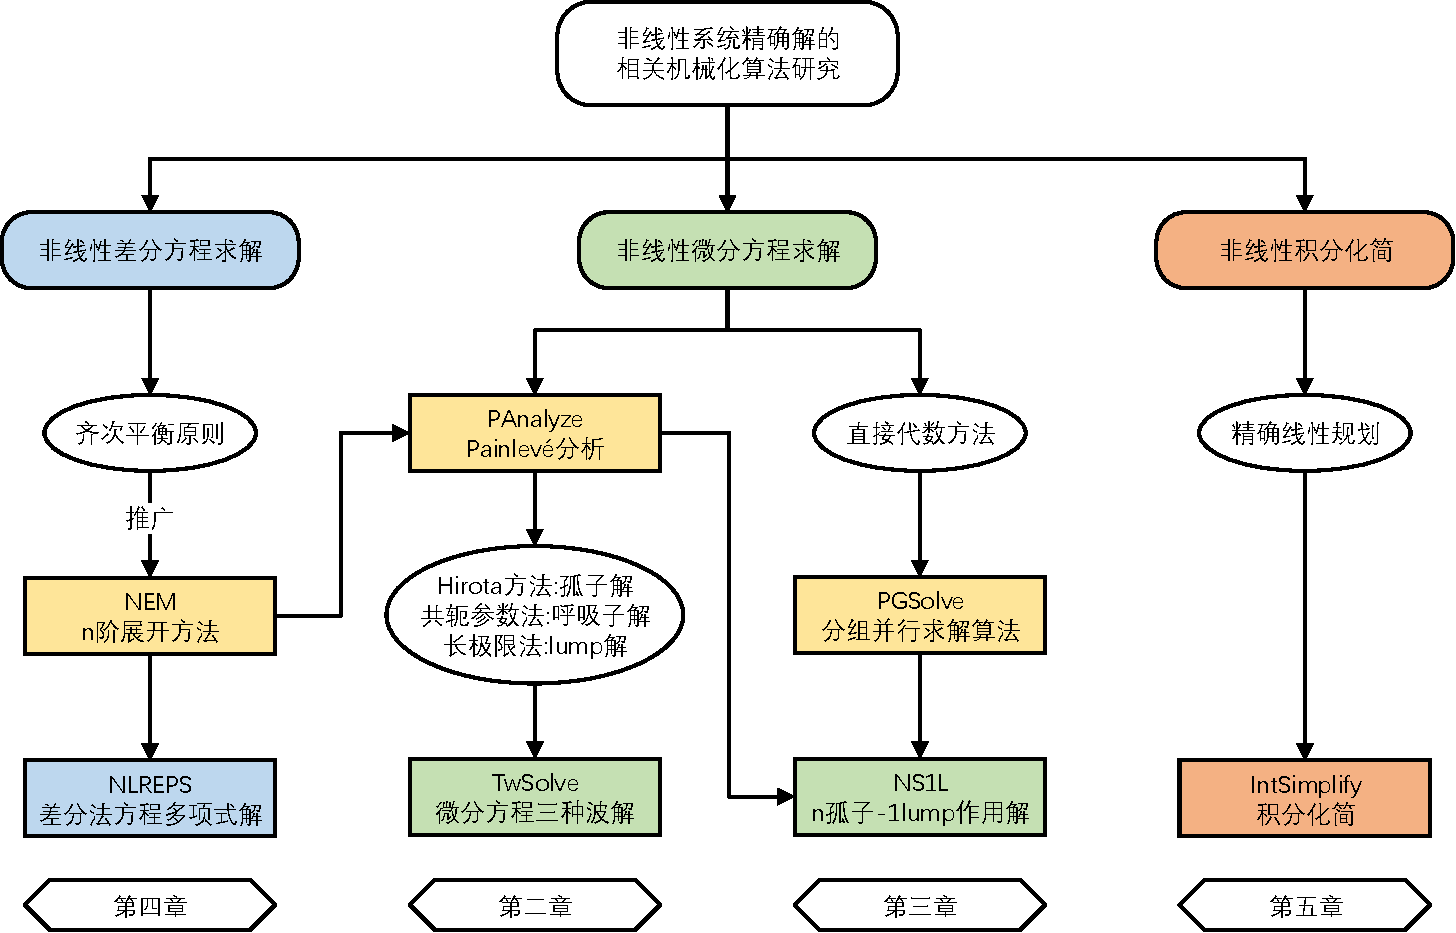
\includegraphics[width=\textwidth]{fig/outline.pdf}
\caption{本文工作大纲图}\label{outline}
\end{figure}


在\refchp{ch02}中, 因为由 Hirota 方法推导出的$n$孤子解公式对可积方程成立, 对不可积方程往往不成立, 本文引入了一种参数约束条件, 将$n$孤子解的公式推广到不可积方程的情形. 在此基础上基于简单Hirota 方法\D 共轭参数法和长极限法, 发展出了构造非线性演化方程的孤子解\D 呼吸子解和 lump 解的机械化算法, 研发了相应的软件包 TwSolver, 并在编程实现时对上述方法的一些细节进行了优化. 


直接代数方法在微分方程的求解中也有广泛的应用, 它的主要难点是其中大规模非线性代数方程组的求解. 在\refchp{ch03}中, 本文针对大规模非线性代数方程组求解困难的问题, 设计了一个分组并行的求解算法, 研发了相应的软件包PGSolve. 作为 PGSolve 的应用实例, 本文开发了用直接代数方法求$n$-孤子和1-lump相互作用解的软件包 NS1L. 

在\refchp{ch04}中, 本文将齐次平衡原则推广为$n$阶展开方法, 并将其应用于微分方程和差分方程的若干求解方法中. 求解微分方程的许多方法都是基于齐次平衡原则发展起来的, 如\Painleve{}展开法\D 双曲正切方法和 Jacobi 椭圆函数方法等. 这些方法将方程的解设为特定函数的多项式, 通过平衡方程中两个不同最高项的阶数来确定解的阶数. 但是, 当一个方程中各个最高项的阶数的表达式相同时, 就无法确定解的阶数的上界, 从而有可能漏解. 本文发现, 解的阶数不仅会出现在最高$n$项的阶数中, 还会出现在最高$n$项的系数中. 因此, 本文考虑同时平衡方程中最高$n$项的阶数和系数, 提出了$n$阶展开方法, 研发了 NEM 软件包. 基于$n$阶展开方法, 进一步提出了一个求解非线性差分方程多项式解的新算法, 并研发了相应的软件包 NLREPS. 同时, 本文还将$n$阶展开方法应用于双曲正切方法和\Painleve{}展开法中. 

因为在非线性微分方程的求解过程中往往需要进行积分表达式的化简, 本文将在第\ref{ch05}章中研究抽象函数积分表达式的化简问题. 首先, 本文建立了一个代数系统将关于抽象函数的积分多项式视为标准积分项的线性组合. 然后, 基于导数的乘法规则, 设计了一个递归算法来寻找所有的二项合并规则. 最后, 基于这些规则将化简问题转化为一个精确线性规划问题进行求解, 实现了非线性积分表达式化简的软件包 IntSimplify.  

\refchp{ch06}对本文完成的工作进行了总结与讨论,概括了本文的主要研究方法和结论,并对未来的工作提出了展望.

需要说明的是, 本文的主线是研究构造非线性微分方程精确解的相关机械化算法. 非线性差分方程多项式解的构造算法及其机械化研究是$n$阶展开方法的推广应用; 而抽象函数的积分多项式化简是为微分方程的化简和求解提供一个辅助工具. 

\section{非线性演化方程的三种波解}
\begin{frame}
\frametitle{非线性演化方程的三种波解}
\begin{enumerate}
\item \Painleve{}展开法得到变换.
\item 简单 Hirota 方法得到孤子解.
\item 共轭参数法得到呼吸子解.
\item 长极限法得到 lump 解.
\end{enumerate}
\end{frame}

\subsection{\Painleve{}展开法}
\begin{frame}
\frametitle{\Painleve{}展开法}
\begin{columns}
\small 
\begin{column}{0.5\textwidth}
理论:
\[
    u=u(x_1,\cdots,x_n,t)
\]
\[
    U(u,u\up{1},u\up{2},u\up{3}\cdots)=0
\]
\[
    u=\sum_{k=1}^m{\frac{u_k}{f^{m-k+1}}}=\frac{u_1}{f^m}+\cdots+\frac{u_m}{f}
\]
\[
    F(f,f\up{1},f\up{2},f\up{3}\cdots)=0
\]
改进:
\begin{itemize}
\item TPE 是对数变换的推广.
\item $m$ 通过$n$阶展开方法确定, 能比齐次平衡原则得到更多的解.
\item 对 $u_k$ 的求解提出了递归算法, 更加全面地考虑了可能出现的情况.
\end{itemize}
\end{column}
\begin{column}{0.5\textwidth}
例子: (3+1) Jimbo-Miwa 方程
\[
    u_{xxxy}+3u_{xx}u_y+3u_{x}u_{xy}+2u_{ty}-3u_{xz}=0
\]
\[
    u=\frac{2f_x}{f}=2\sbrace{\ln f}_x
\]
\[
\begin{split}
    0&=2\,{f}^{2}f_{{{ txy}}}+{f}^{2}f_{{{ xxxxy}}}-3\,{f}^{2}f_{{{ xxz}}}\\
    &-2\,ff_{{t}}f_{{{ xy}}}-2\,ff_{{{ tx}}}f_{{y}}-2\,ff_{{{ ty}}}f_{{x}}\\
    &-4\,ff_{{x}}f_{{{ xxxy}}}+6\,ff_{{x}}f_{{{ xz}}}+3\,ff_{{{ xx}}}f_{{z}}\\
    &+2\,ff_{{{ xxx}}}f_{{{xy}}}-ff_{{{ xxxx}}}f_{{y}}\\
    &+4\,f_{{t}}f_{{x}}f_{{y}}+6\,{f_{{x}}}^{2}f_{{{ xxy}}}-6\,{f_{{x}}}^{2}f_{{z}}\\
    &-6\,f_{{x}}f_{{{ xx}}}f_{{{ xy}}}+2\,f_{{x}}f_{{{ xxx}}}f_{{y}}
\end{split}
\]
\end{column}
\end{columns}
\end{frame}

\subsection{Hirota 方法与孤子解}
\begin{frame}
\frametitle{Hirota 方法与孤子解}
\begin{columns}
\small 
\begin{column}{0.5\textwidth}
行波变换:
\[
\begin{split}
    \xi&=p_1\sbrace{x_1+p_2x_2+\cdots+p_nx_n+\omega t} \\ 
    &+p_{n+1}
\end{split}
\]
\[
    \PS\subseteq  \ALLP=\bbrace{1,2,\cdots,n,n+1}
\]
\[
    S(e,k;\PS): \left\{\begin{array}{ll}
        p_i \rightarrow p_{i,k} & i \in \PS, \\ 
        p_i \rightarrow p_i & i \not\in \PS.
    \end{array}\right.
\]
\[
    \xi_i=S(\xi,i,\PS)
\]
\end{column}
\begin{column}{0.5\textwidth}
例子:
\[
    \xi=k(x+py+qz+\omega t)+c
\]
\[
    \PS=\bbrace{1,2}
\]
\[
\begin{split}
    \xi_i&=k_i\sbrace{x+p_iy+qz+\frac{3q-k_i^2p_i}{2p_i}t}+c, \\ 
    \xi_j&=k_j\sbrace{x+p_jy+qz+\frac{3q-k_j^2p_j}{2p_j}t}+c.
\end{split} 
\]
\end{column}
\end{columns}
\end{frame}

\begin{frame}
孤子解公式:
\[
\begin{split}
    f_{m-soliton}&=\sum_{\mu=0,1}\exp\sbrace{\sum_{i=1}^m{\mu_i \xi_i}+\sum_{1\le i<j\le m}{\mu_i\mu_jH_{i,j}}} \\ 
    &=\sum_{P\subseteq M}\mbrace{\sbrace{\prod_{\bbrace{i,j}\subseteq P}{h_{i,j}}}\exp\sbrace{\sum_{k\in P}{\xi_k}}} \\ 
\end{split}
\]
\[
    M=\bbrace{1,2,\cdots,m},~~\xi_k=S(\xi,k;\PS)
\]
例子:
\[
\begin{split}
    f_1&=1+\exp\sbrace{\xi_1} \\ 
    f_2&=1+\exp\sbrace{\xi_1}+\exp\sbrace{\xi_2}+h_{1,2}\exp\sbrace{\xi_1+\xi_2} \\ 
    f_3&=1+\exp(\xi_1)+\exp(\xi_2)+\exp(\xi_3)\\
       &+h_{1,2}\exp(\xi_1+\xi_2)+h_{2,3}\exp(\xi_2+\xi_3)+h_{1,3}\exp(\xi_1+\xi_3)\\
       &+h_{1,2}h_{2,3}h_{1,3}\exp(\xi_1+\xi_2+\xi_3)
\end{split}
\]
\end{frame}

\begin{frame} 
\[
\begin{split}
    F(f_1)=0 &\Rightarrow \omega \\ 
    F(f_2)=0 &\Rightarrow h_{i,j} 
\end{split}
\]
\[
\begin{split}
    \omega &= \frac{3q-k^2p}{2p} \\ 
    h_{i,j}&=\frac{(k_ip_j(k_i-k_j)+q)p_i^2-p_ip_j(k_jp_j(k_i-k_j)+2q)+qp_j^2}{(k_ip_j(k_i+k_j)+q)p_i^2+p_ip_j(k_jp_j(k_i+k_j)-2q)+qp_j^2}
\end{split}
\]
\begin{figure}
\centering 
\subfigure[1-孤子解 \label{jm:1-soliton}]{
    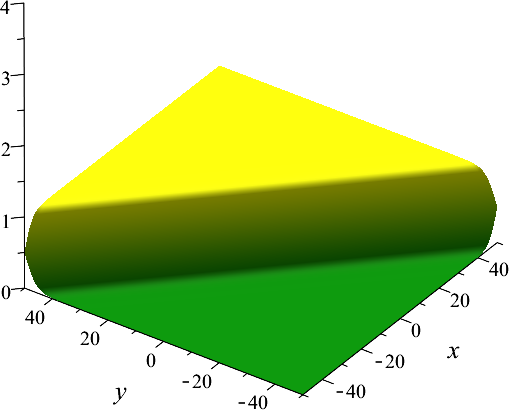
\includegraphics[width=.3\textwidth]{../paper/fig/(3+1)JM-1-soliton.png}    
}
\subfigure[2-孤子解 \label{jm:2-soliton}]{
    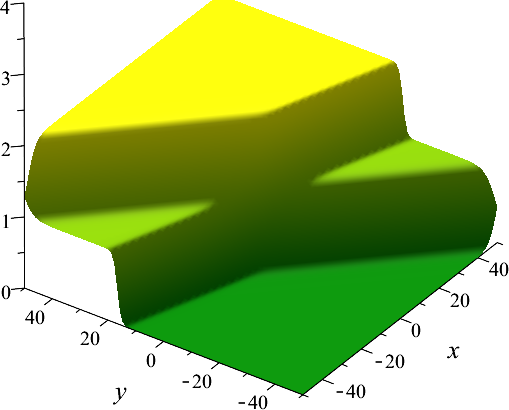
\includegraphics[width=.3\textwidth]{../paper/fig/(3+1)JM-2-soliton.png}
}
\subfigure[3-孤子解 \label{jm:3-soliton}]{
    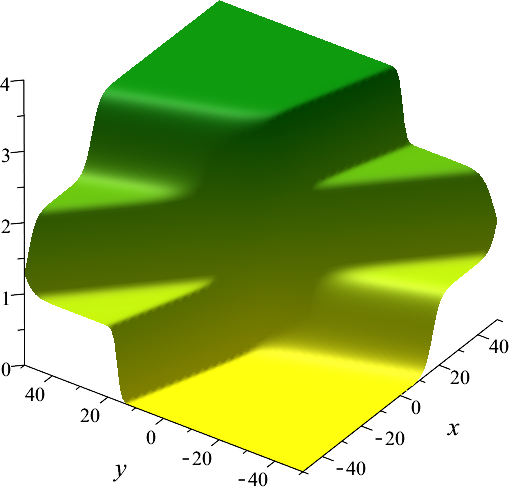
\includegraphics[width=.3\textwidth]{../paper/fig/(3+1)JM-3-soliton.png}
}
\end{figure}
\end{frame}

\subsection{共轭参数法与呼吸子解}
\begin{frame}
\frametitle{共轭参数法与呼吸子解}
\begin{columns}
\begin{column}{0.5\textwidth}
理论:
\[
    f_{m-breather}=\conj{f_{(2m)-soliton}} 
\]
\[
    p_{i,j}=p_{i,j+m}^*,~(j=1,2,\cdots,m)
\]
\[
\begin{split}
    p_{i,j}&=p_{i,j,RE}+I\cdot p_{i,j,IM}, \\ 
    p_{i,j+m}&=p_{i,j,RE}-I\cdot p_{i,j,IM},
\end{split}
\]
\end{column}
\begin{column}{0.5\textwidth}
例子: $m=1,\PS=\bbrace{1,2}$,\\$\xi=k(x+py+qz+\omega t)+c$.
\[
\begin{split}
    k_1&=k_{1,RE}+I\cdot k_{1,IM} \\ 
    k_2&=k_{1,RE}-I\cdot k_{1,IM} \\
    p_1&=p_{1,RE}-I\cdot p_{1,IM} \\
    p_2&=p_{1,RE}+I\cdot p_{1,IM} \\ 
\end{split} 
\]
\end{column}
\end{columns}
\end{frame}

\begin{frame}
\begin{figure}
\setcounter{subfigure}{0}
\subfigure[1-呼吸子解 \label{jm:1-breather}]{
    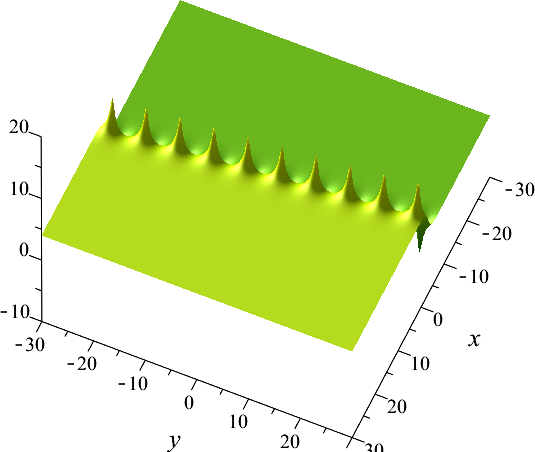
\includegraphics[width=.3\textwidth]{../paper/fig/(3+1)JM-1-breather.png}
}
\subfigure[2-呼吸子解 \label{jm:2-breather}]{
    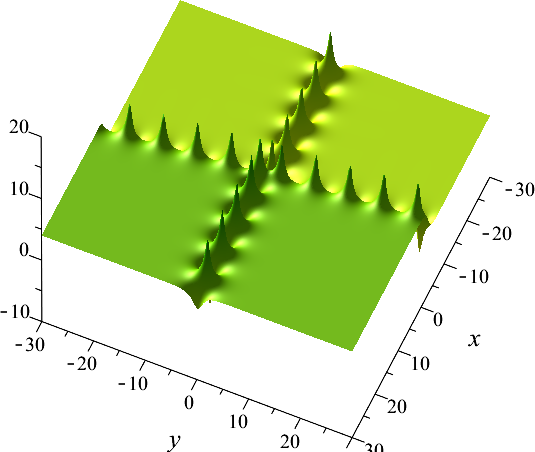
\includegraphics[width=.3\textwidth]{../paper/fig/(3+1)JM-2-breather.png}
}
\subfigure[3-呼吸子解 \label{jm:3-breather}]{
    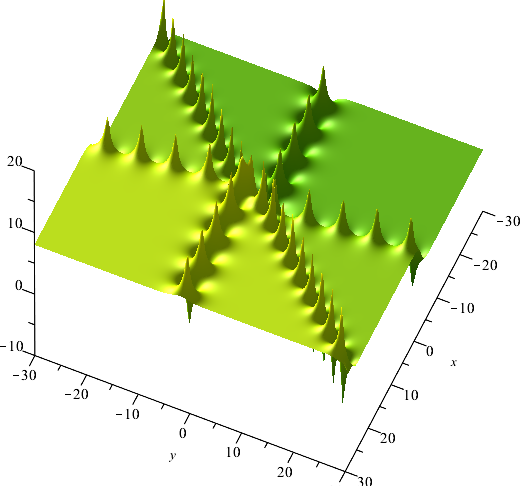
\includegraphics[width=.3\textwidth]{../paper/fig/(3+1)JM-3-breather.png}
}
\subfigure[周期波解 \label{jm:1-periodic}]{
    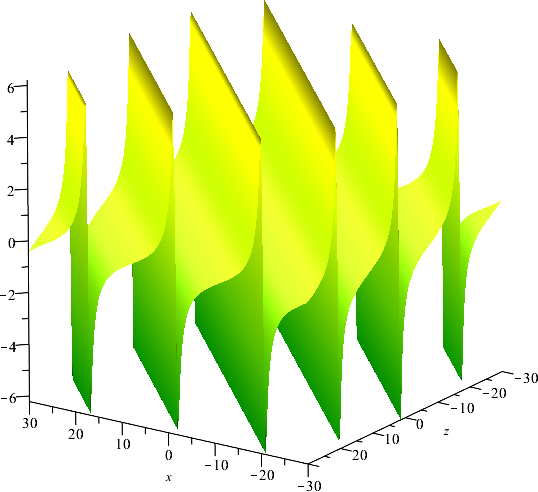
\includegraphics[width=.3\textwidth]{../paper/fig/(3+1)JM-1-periodic.png}
}
\subfigure[孤子-呼吸子相互作用解 \label{jm:soliton-breather}]{
    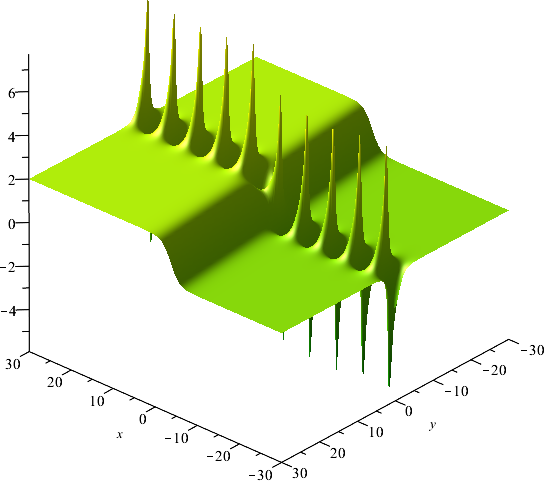
\includegraphics[width=.3\textwidth]{../paper/fig/(3+1)JM-soliton-breather.png}
}
\end{figure}
\end{frame}

\subsection{长极限法与 lump 解}
\begin{frame}
\frametitle{长极限法与 lump 解}
生成公式:
\[
    f_{m-lump}=\conj{\Theta_m}
\]
\[
\begin{split}
    \Theta_m&=\prod_{k=1}^{2m}\theta_k+\frac{1}{2}\sum_{i,j}{b_{i,j}}\prod_{J\neq i,j}{\theta_J}+\frac{1}{2! 2^2}\sum_{i,j,k,l}{b_{i,j}b_{k,l}}\prod_{J\neq i,j,k,l}{\theta_{J}}+\cdots \\
    &+\frac{1}{s!2^s}\sum_{i,j,\cdots,u,v}\underbrace{{b_{i,j}b_{k,l}\cdots b_{u,v}}}_{s}\prod_{J\neq i,j,\cdots, u,v}{\theta_J}+\cdots 
\end{split}
\]
例子:
\[
\begin{split}
\Theta_1&=\theta_{1}\theta_{2}+b_{12} \\
\Theta_2&=\theta_{1}\theta_{2}\theta_{3}\theta_{4}+b_{12}\theta_{3}\theta_{4}+b_{13}\theta_{2}\theta_{4}+b_{14}\theta_{2}\theta_{3}+b_{23}\theta_{1}\theta_{4}\\
&+b_{24}\theta_{1}\theta_{3}+b_{34}\theta_{1}\theta_{2}+b_{12}b_{34}+b_{13}b_{34}+b_{14}b_{23}
\end{split}
\]
\end{frame}

\begin{frame}
重写生成公式
\[
    f_{m-lump}=\sum_{l=0}^m\sum_{s\in L(l)}\sbrace{\prod_{k=1}^l{b_{s_{2k-1},s_{2k}}}\prod_{p\not\in s}{\theta_p}}
\]
\[
    L(l)=\bbrace{\sbrace{s_1, s_2, \cdots ,s_{2l}}\left|s_{2k}>s_{2k-1},s_{2k+1}>s_{2k-1},s_k\in \bbrace{1,\cdots,2l}\right.}
\]
\begin{itemize}
\item $s_{2k}>s_{2k-1}$ 保证了$b_{i,j}=b_{j,i}$的等价情况只出现一次. 
\item $s_{2k+1}>s_{2k-1}$ 保证了$b_{i,j}$的全排列只出现一次.
\end{itemize}
\end{frame}

\begin{frame}
\begin{columns}
\begin{column}{0.5\textwidth}
关键参数:
\[
\begin{split}
    \theta &= \eval{\frac{\partial \xi}{\partial p_1}}{p_1=0}, \\
    b_{i,j}&= \eval{\frac{\partial^2}{\partial p_{1,i}\partial p_{1,j}}h_{i,j}}{p_{1,i}=0,p_{1,j}=0}.
\end{split}
\]
\end{column}
\begin{column}{0.5\textwidth}
例子:
\[
\begin{split}
    &\theta=\frac{2p^2y+(2qz+2x)p+3qt}{2p}, \\ 
    &b_{i,j}=-\frac{2p_ip_j(p_i+p_j)}{q(p_i-p_j)^2}.
\end{split}
\]
\end{column}
\end{columns}
\begin{figure}
\setcounter{subfigure}{0}
\centering 
\subfigure[1-lump解 \label{jm:1-lump}]{
    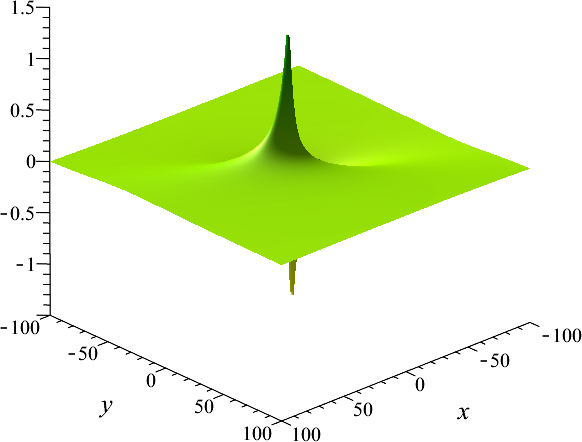
\includegraphics[width=.3\textwidth]{../paper/fig/(3+1)JM-1-lump.png}
}
\subfigure[2-lump解 \label{jm:2-lump}]{
    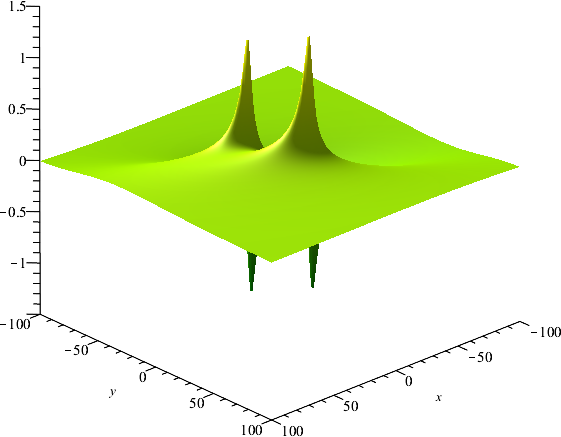
\includegraphics[width=.3\textwidth]{../paper/fig/(3+1)JM-2-lump.png}
}
\subfigure[3-lump解 \label{jm:3-lump}]{
    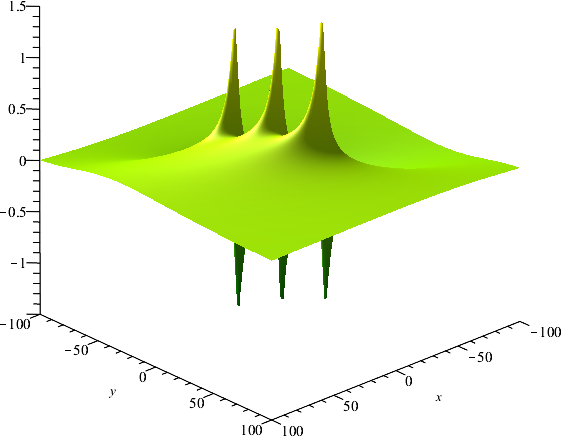
\includegraphics[width=.3\textwidth]{../paper/fig/(3+1)JM-3-lump.png}
}
\end{figure}
\end{frame}

\subsection{实验与分析}
\begin{frame}
\frametitle{实验与分析}
\begin{columns}
\begin{column}{0.65\textwidth}
\begin{table}
\centering
\small 
\begin{tabular}{lcccc}
\hline
\multicolumn{1}{c}{方程名} & 1 & 12 & 13 & 123 \\ 
\hline
(1+1)KdV & \tpa\tpb & & & \\
(2+1)BKP-T & \tpa\tpb & \tpa\tpa & & \\
(2+1)KP &\tpa\tpb &\tpa\tpa & & \\
(2+1)SK &\tpa\tpb &\tpa\tpa & & \\
(4+1)Fokas-T-2 &\tpa\tpb &\tpa\tpa & & \\
(2+1)CBS & \tpa\tpb & \tpa\tpb & & \\
(2+1)CBS-G & \tpa\tpb & \tpc\tpc & & \\
(3+1)BKP &\tpa\tpb &\tpa\tpa &\tpa\tpa &\tpc\tpc \\
(3+1)KP &\tpa\tpb &\tpa\tpa &\tpa\tpa &\tpc\tpc \\
(3+1)JM &\tpa\tpb &\tpa\tpa &\tpa\tpb &\tpc\tpc \\
(3+1)NEE-T &\tpa\tpb &\tpa\tpa &\tpa\tpb &\tpc\tpc \\
(3+1)YTSF &\tpa\tpb &\tpa\tpa &\tpa\tpb &\tpb\,\tpb \\
(3+1)CBS &\tpa\tpb &\tpa\tpb &\tpa\tpb &\tpa\tpb \\
(4+1)Fokas-T &\tpa\tpb &\tpa\tpb &\tpa\tpb &\tpc\tpc \\
\hline
\end{tabular}
\end{table}
\end{column}
\begin{column}{0.35\textwidth}
\begin{itemize}
\item `\tpa{}' 表示能够满足原方程.
\item `\tpb{}' 表示有解不能得到解.
\item `\tpc{}' 表示有解但不满足原方程.
\item 第一个对应3孤子解, 第二个对应2 lump解.
\end{itemize}
\end{column}
\end{columns}
\end{frame}
\chapter{分组并行求解算法及其应用}\label{ch03}
在微分方程的求解中, 许多方法最终都能归结于代数方程组的求解. 这些求解方法的主要困难在于最终的代数方程组规模过大, 无法在有限的时间内求解. 为了解决这个问题, 本文提出了一个分组并行的求解算法, 并将其实现为 PGSolve 软件包. 然后, 本文以求$n$-孤子和1-lump相互作用解的直接代数方法为例, 展示了 PGSolve 在大规模代数方程组求解时的效率. \todo{也可以举一代数方法软件包的例子}

\section{分组并行求解算法与PGSolve软件包}
代数方程组的求解是符号计算的核心问题之一. 尤其是多项式代数方程组的求解, 更是符号计算中最基础也是最困难的问题. 多项式代数方程组的求解算法有吴文俊先生的吴方法\cite{wu1984,wu1985}\D 正则列方法\cite{kalkbrener1991three,lu1994searching}和\Grobner{}基方法\cite{adams1994introduction}等. 吴方法的实现有王东明的charsets\cite{wang1995implementation}和王定康的wsolve\cite{wsolve}等. 正则列方法的实现有 RegularChains \cite{maza2000triangular}, 该软件包已经被包含在 Maple 的内置函数中. 求\Grobner{}基的相关算法有 Buchberger 算法\cite{buchberger1970algorithmic}\D F4 算法\cite{faugere1999new} 和 F5 算法\cite{faugere2002new}等. Maple 和 Mathematica 等计算机代数系统的内置求解函数都是以\Grobner{}基方法为基础实现的, 且\Grobner{}基方法不仅能够求解多项式方程组, 还能求解更加一般的代数方程组. 

上述方法的基本原理是将原方程组转化一个或多个三角化的方程组后在逐个求解, 且三角化后的方程组和原方程组同解. 但是, 算法关于方程组规模的时间复杂度都是指数的, 并且计算过程中表达式的中间结果膨胀十分严重, 难以在有限的时间和内存条件下求解大规模的方程组. 并且, 上述算法注重数学上的严谨性, 致力于求解原方程组所有的解. 然而在实际求解过程中, 我们往往只需要一部分的解, 这些算法在解的完整性上的优势反而成为了降低求解效率的重要原因. 

因此, 为了高效地从大规模的代数方程组中解得用户想要的解, 本文基于如下几点想法, 提出了一个分组并行的求解算法.
\begin{compactenum}[(1)]
\item 对原方程组进行合理的分组后依次求解, 完成一个分组的求解后, 将解代入剩余的方程中继续求解. 
\item 在求解过程中删除不满足用户要求的解, 以减少解的分支, 提高求解效率.
\item 在适当的步骤中采用并行策略进行加速, 充分利用多核计算机的性能.
\end{compactenum}

\subsection{核心框架}
\begin{figure}[htbp]
\centering 
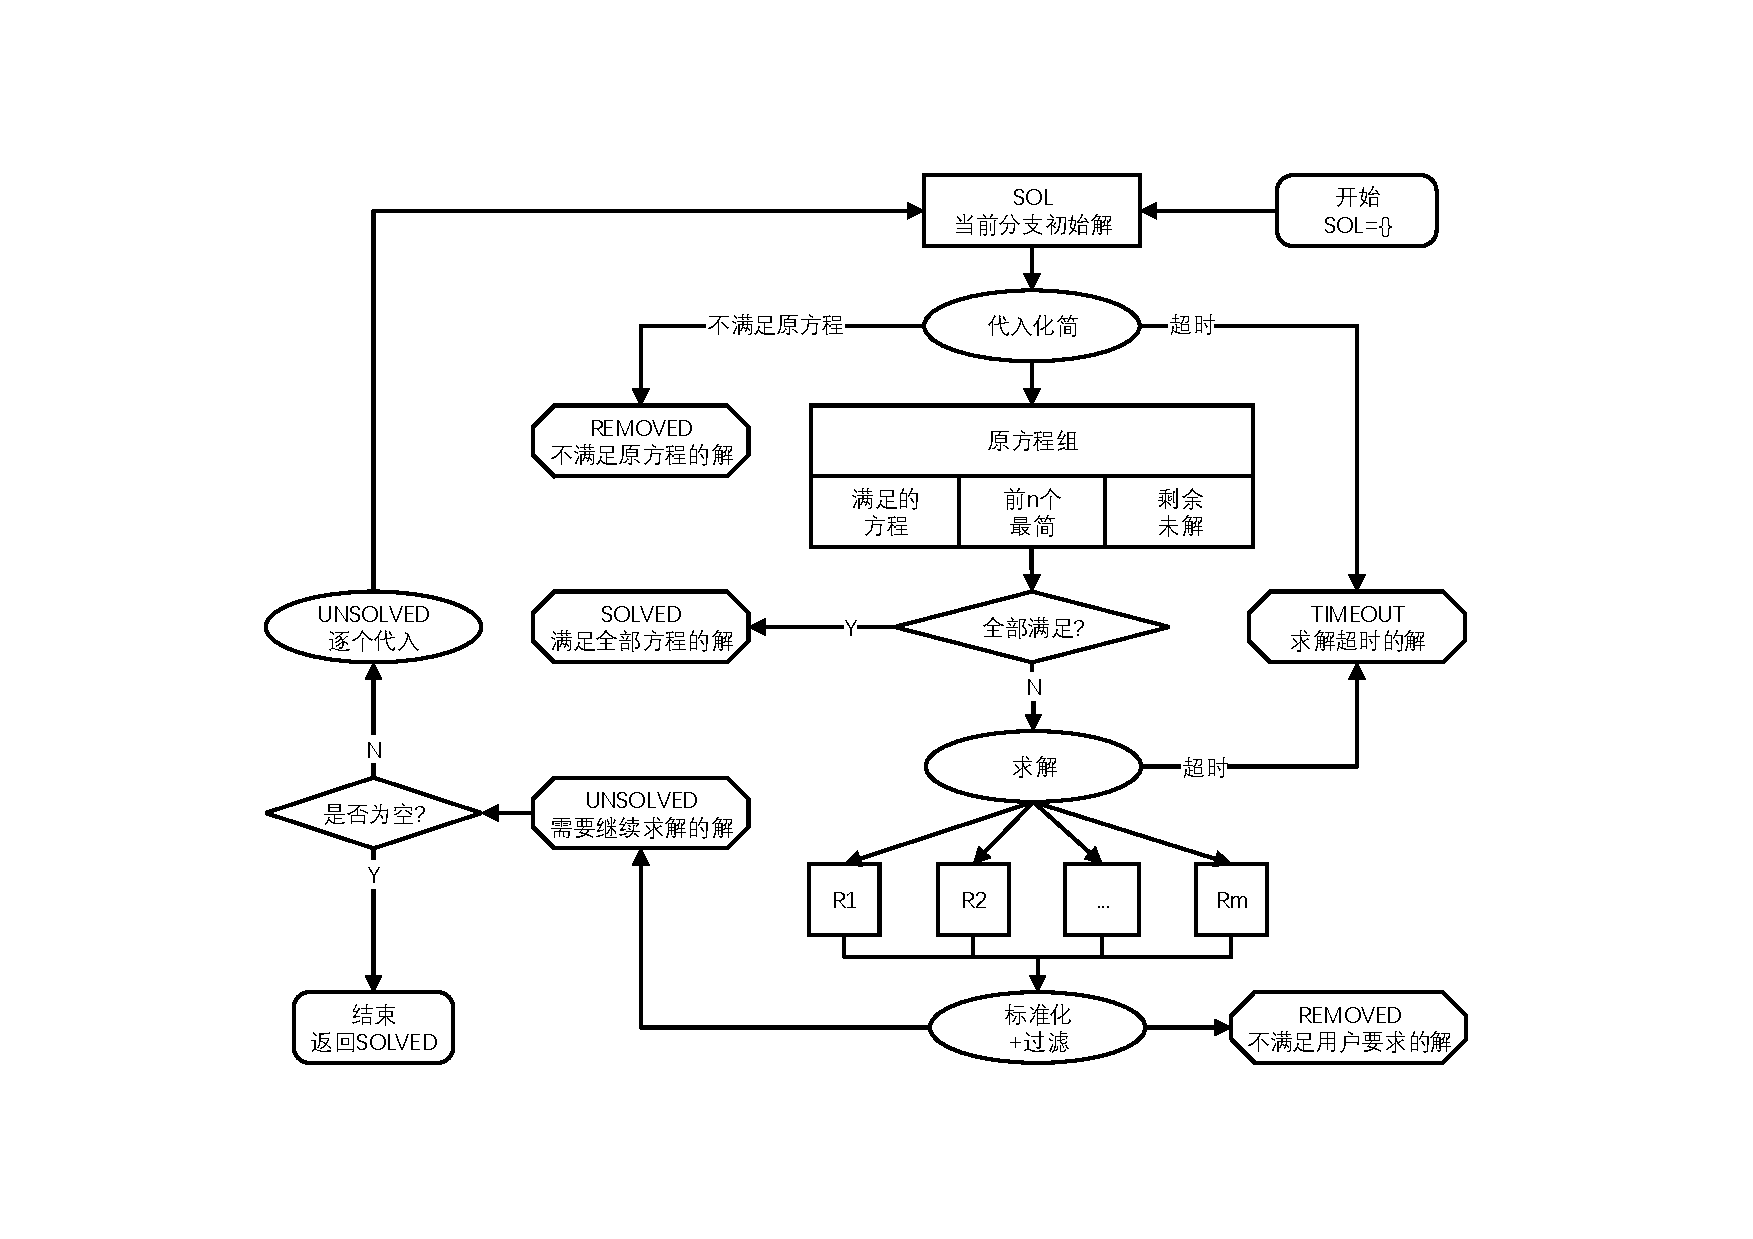
\includegraphics[width=0.9\textwidth]{fig/pgsolve.pdf}
\caption{PGSolve 算法框架}\label{PGSolve}
\end{figure}

根据上文的讨论, 本文设计了如\reffig{PGSolve}所示的算法框架. 该算法的具体步骤如下:
\begin{compactenum}[Step 1.]
\item 初始化: 用于保存解集的 SOLVED\D UNSOLVED 以及 TIMEOUT 三个容器为空集. 令 SOL=\{\}. 
\item 将当前解SOL代入原方程组之后并化简. 化简之后, 原方程组可以分为三个部分. 第一部分是已经满足的方程, 这些方程在代入化简后为零. 将剩余的方程按照复杂度进行升序排序之后, 可以根据用户给定的n分为两个部分. 
\item 在代入化简后, 
    \begin{compactenum}[(a)]
    \item 如果存在一些方程的化简结果为常数, 则表示SOL不满足原方程组, 我们将其废弃后进入下一个分支的求解. 
    \item 若SOL满足原方程组的所有方程, 则将 SOL 加入 SOLVED之后继续下一个分支的求解. 
    \item 若化简超时, 则将 SOL 加入 TIMEOUT 后继续下一个分支的求解. 
    \item 否则, 就取尚未求解的方程中最简单的n个进行求解.
    \end{compactenum}
\item 若求解超时, 则将 SOL 加入 TIMEOUT. 否则, 就对求得的解进行标准化. 标准化包含以下几个步骤:
    \begin{compactenum}[(1)]
    \item 删除每个解中的自由变量. 这是因为 Maple 的 solve 在求解时会返回自由变量(如 x=x).
    \item res 中的每个解并上 sol 构成一个新的方程, 再利用 solve 进行求解, 保证解的最简性和唯一性. 
    \item 再次删除自由变量.
    \item 按照用户指定条件对解进行过滤, 删除不满足用户指定条件的解. 
    \end{compactenum}
\item 标准化之后, 按照用户给定的条件对解进行过滤, 将满足条件的解加入 UNSOLVED 继续求解. 
\item 如果此时 UNSOLVED 为空, 则算法结束, SOLVED 中包含了用户想要的解. 否则, 就将 UNSOLVED 内的元素全部取出之后, 依次作为 SOL 转 Step 2 继续求解. 
\end{compactenum}


在上述算法中, 我们对代入化简后的方程组按照复杂度升序进行排序. 其目的在于降低求解的前$n$个方程所构成的方程组的复杂度.  因为要想利用分组策略提高方程组的求解效率, 就需要满足以下两个条件: (1) 前面的分组尽可能的简单, 减少单步的求解时间; (2) 前面的分组解所得的解尽可能的少, 以减小求解分支的数量. 

一个方程组的复杂度是由三个个方面决定的: 一方面是方程的数量, 方程的数量越多方程组就越复杂; 另一方面是方程组中变量的个数, 变量的个数越多则方程组越复杂; 还有一方面是方程组中表达式的复杂度, 单个表达式长度越长, 次数越高, 则这个表达式越复杂. 出于这些考虑, 按复杂度排序的逻辑如下:
\begin{compactenum}[(1)]
\item 将方程按照变量进行分组, 变量相同的方程放在同一组内.
\item 将上述分组按照变量数量升序排序.
\item 每个分组内利用 Maple 的 \cd{SolveTools:-Complexity} 函数衡量表达式的复杂度, 按照复杂度升序排序.  
\item 上述操作完成后, 将各个分组展开, 把方程组还原为一个列表. 
\end{compactenum}

按照上述策略进行排序就能保证所求解的前$n$个方程构成的方程组是最简的. 接着, 我们就要尽可能地控制解的数量以减少分支的数量. 在变量数目不变的情况下, 一个方程组解的数量和方程的数量相关. 一般而言, 方程数量越多, 约束约苛刻, 则解的数量就越少. 但是方程数量越多, 则求解这个方程组所需要的时间越长. 因此, 求解方程的数量是一个需要权衡的数字, 可以由用户根据实际情况进行设置, 而本文一般取 $n=5$.

此外需要特别说明的是, 我们将SOL代入所有的方程进行代入化简的主要原因如下: 
\begin{compactenum}[(1)]
\item 对尚未求解的方程进行代入化简, 能够对新的方程组按照复杂度重新排序, 从而获得更简单的方程.
\item 对已经求解过的方程进行代入化简, 能够验证当前分支的解是否满足这部分方程. 
\item 以便在获得原方程的解时直接返回. 此时, 尽管我们只求解了部分方程, 但是求得的解能够全部方程时, 就能提起阶数分支, 将当前的解添加到 SOLVED 中. 
\end{compactenum} 

而在 TIMEOUT 中保存超时的解的意义在于, 如果用户在求解结束时愿意花更多的时间来继续求解超时的解, 就将 TIMEOUT 赋值给 UNSOLVED 之后, 设定更大的时限重新求解. 

\subsection{并行调度策略} 
在\reffig{PGSolve}所示的算法中, 除了``求解''以外的三个椭圆形节点所代表的步骤都能够并行化. 在实际求解过程中, 
\begin{compactitem}[\textbullet]
\item ``代入化简''所需的时间最长, 而化简一个表达是又是一个工作量比较小的原子任务, 比较适合将其并行化.
\item ``标准化+过滤''所需的时间极短, 并行加速的意义不大.
\item ``UNSOLVED逐个代入''这个步骤的每个子任务所包含的工作量过大, 不适合并行加速.
\end{compactitem}
因此, 我们选择将``代入化简''这一步并行化. 而我们所采用的并行调度策略是经典的Master-Slave调度模型\cite{sahni1996master}. 

如\reffig{msp}所示, Master-Slave 调度模型的原理如下:
\begin{compactenum}[Step 1.]
\item 所有并行任务进入任务池.
\item Master 节点从任务池拉取任务分配给空闲的 Slave 节点, 直到没有空闲节点.
\item Slave 完成任务后返回, Master 将新的任务分配给当前 Slave 节点, 直至所有任务完成. 
\end{compactenum}

\begin{figure}[htbp]
\centering 
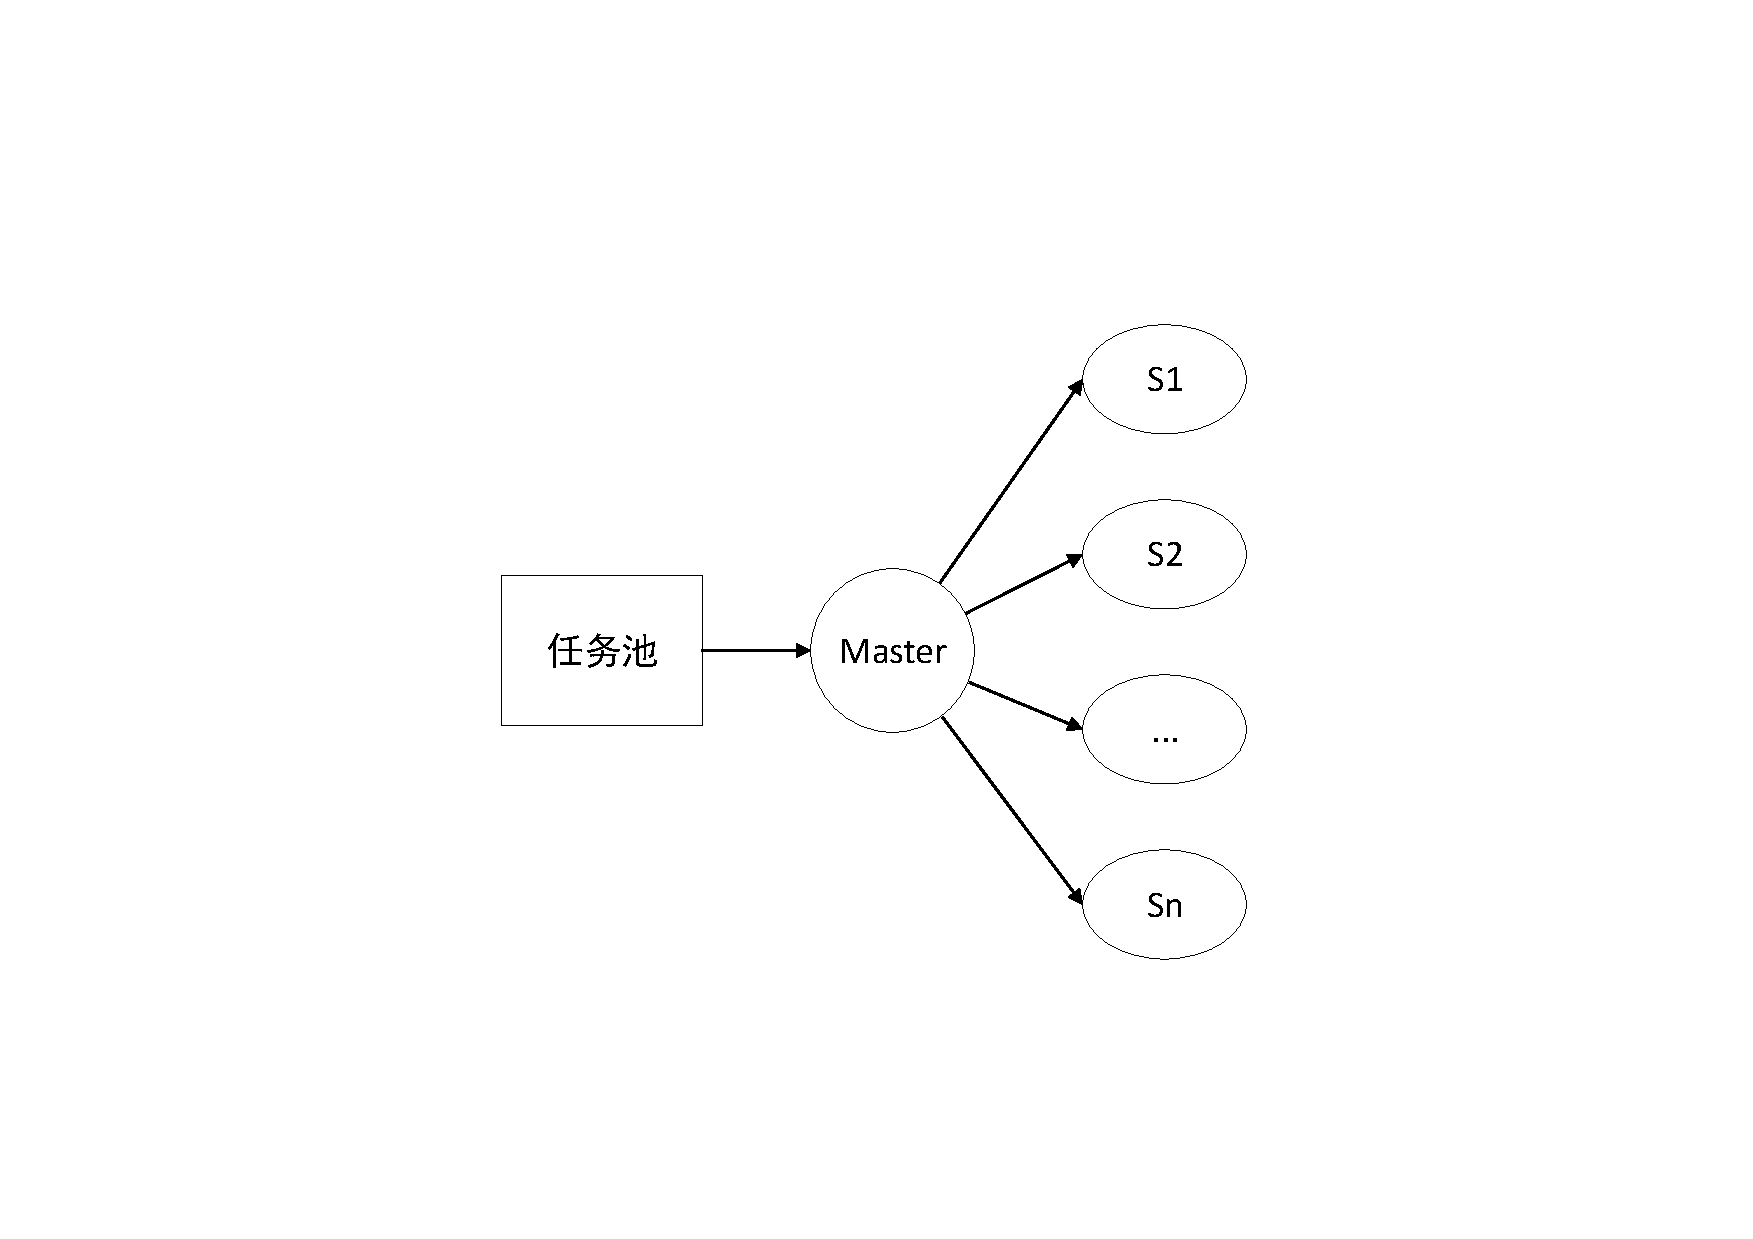
\includegraphics[width=0.5\textwidth]{fig/msp.pdf}
\caption{Master-Slave 调度模型}\label{msp}
\end{figure}

\subsection{PGSolve软件包的接口与实现}
根据上文所述的算法, 我们在 Maple 中实现了 PGSolve 软件包. PGSolve 软件包的核心接口是 \cd{GroupSolver} 对象, 该对象实现了\reffig{PGSolve} 所述的功能. \cd{GroupSolver}的构造函数为: 
\begin{verbatim}
GroupSolver(eqs,vrs,filter,{use_parallel});
\end{verbatim}
其中, 
\begin{compactitem}[\textbullet]
\item \cd{eqs} 表示方程组;
\item \cd{vrs} 表示需要求解的变量的集合;
\item \cd{filter} 是一个用户自定义的函数, 对需要删除的解返回 \cd{true}, 对需要保留的解返回 \cd{false};
\item 选项 \cd{use\_parallel} 是可选的, 当用户指定这个选项时, \cd{GroupSolver} 才会在求解时采用并行策略进行加速.
\end{compactitem}
当 \cd{GroupSolver} 的构造完成时, 它会将 \cd{eqs, vrs, filter} 作为成员变量进行存储, 同时初始化 SOLVED\D UNSOLVED 和 TIMEOUT 三个解的集合. 

当 \cd{GroupSolver} 构造完成后, 用户就可以调用 \cd{GroupSolver:-agsolve(n,TL)} 实现自动求解, 调用 \cd{GroupSolver:-pgsolve(n,TL)} 实现分步求解. 其中, \cd{n}表示分组求解的个数, 而\cd{TL}表示单步求解的最长时间.  \cd{GroupSolver:-agsolve} 对应实现了\reffig{PGSolve}的全部流程, 而 \cd{GroupSolver:-pgsolve} 实现的则是从``SOL''节点开始到``是否为空?''的流程. 使用 \cd{agsolve} 的优势在于整个求解流程自动完成, 缺点在于不能中途调整 \cd{n} 和 \cd{TL}. 而 \cd{pgsolve} 则可以根据求解情况, 设置不同的 \cd{n} 和 \cd{TL} 进行求解. 

在Maple中, 并行可以分为基于 \cd{Threads} 软件包的多线程并行和基于 \cd{Grid} 软件包的多进程并行. 多线程并行可以进行资源共享, 但当多个线程同时访问一个资源时会存在线程安全的问题, 有可能导致程序出错. 因为 Maple 中许多重要的内置函数(如, \cd{solve})都不是线程安全的, 因此我们选择采用多进程并行. 多进程并行不存在资源共享的问题, 进程之间的交流靠通信实现. 尽管 \cd{Grid} 软件包中有 \cd{Map} 这样一个高级接口可以直接实现基于 Master-Slave 调度模型的并行过程, 但是为了控制整个计算过程的时长, 我们还是自行实现了一个 \cd{pmap} 函数. 该函数的调用方式为 \cd{pmap(f,v,TL)}. 其中, \cd{f} 是作用在列表 \cd{v} 中每个元素上的函数, 而 \cd{TL} 则是总的时间限制. \cd{GroupSolver} 中的并行过程就是基于 \cd{pmap} 函数实现的. 

\section{求 $n$-孤子和 1-lump 相互作用解的直接代数方法}
在微分方程的求解过程中, 许多方法最终都归结于代数方程组的求解. 包括齐次平衡方法\D 双曲正切方法和 Jacobi椭圆函数方法等, 最终都需要求解代数方程组. 不过这些方法最终的方程组规模都不大, 本文就不以它们举例了. 我们在\refchp{ch02}中, 基于简单 Hirota 方法求得了 NLEE 的孤子解\D 呼吸子解和lump 解. 其实, 我们也能通过直接代数方法来求解它们. 不过, 显然是\refchp{ch02}中的算法求解方法效率更高. 但是, 对于孤子解和lump解的相互作用解, 目前就只能利用直接代数方法进行求解. 由于求解该问题能够产生大规模的代数方程组, 我们就以该问题为例来展示 PGSolve 的作用, 同时测试 PGSolve 的有效性. 

采用直接代数方法求 $n$-孤子和 1-lump 相互作用解的第一步和\refchp{ch02}中的简单 Hirota 方法一样, 都是利用 \Painleve{} 分析确定变换. 然后, 若自变量为$x_1,\cdots,x_m$, 则解的假设形式为
\begin{equation}
f_n=\sbrace{\xi_1+\eta_1}^2+\sbrace{\xi_2+\eta_2}^2+\sum_{i=1}^{2^n}\sbrace {q_i\prod_{k \in P_i}{\exp(\xi_{k+2})}}. \label{f-ns1l}
\end{equation}
其中, $P_i$ 是 $\bbrace{1,\cdots,n}$的全体子集中的第$i$个, 而
\begin{equation}
\xi_k=\sum_{j=1}^m{p_{j,k}x_j}.
\end{equation}
在\refeqn{f-ns1l}中, 前两个平方项的和构成了lump解的部分, 而最后一个求和项则是孤子解的部分. 在该假设形式中, 待定参数的集合为
\begin{equation}
    \bbrace{q_i|1\le i \le 2^n} \cup \bbrace{p_{j,k}|1\le j \le m, 1\le k \le n+2} \cup \bbrace{\eta_1,\eta_2}. 
\end{equation}

值得说明的是, 本文是在\refchp{ch02}中多孤子解的生成公式\ref{f-soliton-new}的基础上给出\refeqn{f-ns1l}的. \refeqn{f-ns1l}的优点在于让高阶的解在某些参数取零时, 能够退化为相同形式的低阶解. 例如,
\begin{equation}
    f_1=\sbrace{\xi_1+\eta_1}^2+\sbrace{\xi_2+\eta_2}^2+q_1+q_2 \exp(\xi_3)
\end{equation}
在取$q_2=0$时, 可以退化为
\begin{equation}
    f_0=\sbrace{\xi_1+\eta_1}^2+\sbrace{\xi_2+\eta_2}^2+q_1.
\end{equation}
要想达到上述效果, 就需要对 $\bbrace{1,\cdots,n}$ 的全体子集进行合适的排序. 事实上, 按照\refalg{allsubset}生成的子集能够满足上述要求. 在\refalg{allsubset}中, 我们假设并集操作会保留元素的顺序. 

\begin{algorithm}
\caption{NS1L中的全体子集生成算法}\label{allsubset}
\Fn{$allsubset(n)$}{
    \lIf{$n=0$}{
        \Return{$\bbrace{\emptyset}$}
    }
    $X\gets allsubset(n-1)$\;
    \Return{$X \cup  \sbrace{\bigcup\limits_{v\in X}{v \cup \{n\}}}$}\;
}
\end{algorithm}

在确定了解的假设形式之后, 我们需要确定参数的约束条件. 按照相互作用解的实际意义, 需要满足:
\begin{compactenum}[(1)]
\item 孤子解的各个组成部分非零. 即$q_i\neq 0~(i=1,\cdots,2^n)$.
\item lump 的各个组成部分非零, 即$\xi_1\neq 0,\xi_2\neq 0$.
\item 孤子解的各个孤子非零, 即$\xi_k\neq 0~(k=3,\cdots,n+2)$.
\item 孤子解部分和lump解部分解的维数不能退化, 即自变量的数量不能减少. 
\end{compactenum}

为了筛选出满足上述条件的解, 我们提出一个\emph{避免取值集合}的概念. 给定一个\emph{避免取值集合}$S$, 对于原方程组的一个解$t$ (是一个集合), 若存在$s\in S$, 满足$s\subseteq t$, 则$t$就不是我们想要的解. 而在我们的问题中, 
\begin{equation}
\begin{split}
    S&=\bbrace{\bbrace{q_i=0}|1\le i \le 2^n} \\ 
     &\cup \bbrace{\bbrace{p_{1,k}=0,\cdots,p_{m,k}=0}|1\le k \le n+2}  \\
     &\cup \bbrace{\bbrace{p_{j,1}=0,p_{j,2}=0}|1\le j \le m} \\ 
     &\cup \bbrace{\bbrace{p_{j,3}=0,\cdots,p_{j,n+2}=0}|1\le j \le m} . 
\end{split}
\end{equation}
式中第一个集合保证了孤子解的各个组成部分非零, 第二个集合保证了各个孤子非零以及lump解的各个部分非零, 第三个集合保证了lump解部分维数不退化, 而第四个集合保证了孤子解部分维数不退化.

\section{NS1L 和 PGSolve 软件包的应用实例}
基于上一节中的理论分析, 结合本文在 TwSolver 和 PGSolve 软件包上的工作, 我们开发了能够求解非线性演化方程 $n$-孤子和 1-lump 相互作用解的软件包 NS1L. 下面, 本文将以一个具体方程为例, 展示 NS1L 的调用方式, 同时测试 PGSolve 的求解性能. 此外, 在下文中, 我们将简称 n-孤子和 1-lump 的相互作用解为 nS-1L 解. 

\subsection{基本用法}
考虑(3+1)YTSF方程\CITEcaYTSF,
\begin{equation}
    3\,\alpha\,u_{{{\it yy}}}+4\,u_{{x}}u_{{{\it xz}}}+2\,u_{{{\it xx}}}u_{{z}}-4\,u_{{{\it tx}}}+u_{{{\it xxxz}}}=0. 
\end{equation}

因为NS1L中也可以取$n=0$, 所以我们先以0S-1L解(即 lump 解)为例进行求解. 

Step 1. 生成代数方程组.
\begin{verbatim}
sh:=gen_eq(eq,0,p,q);
\end{verbatim}
这里, \cd{gen\_eq} 的第一个参数是一个NLEE, 第二个参数\cd{n}表示相互作用解中孤子解的阶数. 而\cd{p,q}则对应\refeqn{f-ns1l}中的$p,q$, 用于给待定参数设置变量名. 而返回值\cd{sh}是一个\cd{EqnHolder}对象. 该对象的作用类似于TwSolver中的\cd{SolHolder}对象, 我们接下来将一一展示它的作用. 

Step 2. 求解代数方程组.
\begin{verbatim}
ph:=sh:-get_solver();
sols:=ph:-agsolve(5);
\end{verbatim}
这里的第一行我们先利用\cd{EqnHolder}对象获得求解对应代数方程组的\cd{GroupSolver}对象. 其实, 我们还能通过\cd{sh:-get\_solver(use\_parallel)}来获得使用并行策略进行加速的\cd{GroupSolver}对象. 第二行再通过调用PGSolve中的\cd{GroupSolver}对象进行代数方程组的求解. 在求lump解时, 共有35个方程和11个待定参数, \cd{GroupSolver}能够在1秒左右求得3组解. 对于这个例子, PGSolve 在求解时的分支图如\reffig{sb0}所示. 

\begin{figure}[htbp]
\centering
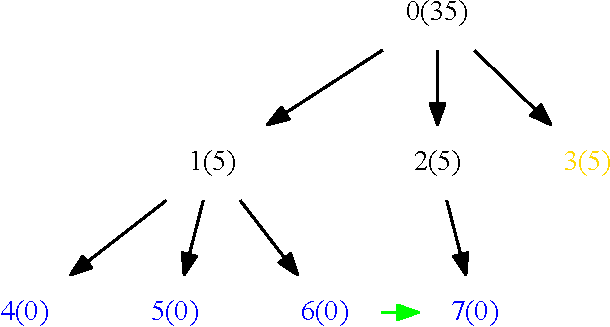
\includegraphics[width=.3\textwidth]{fig/0S1L.pdf}
\caption{(3+1)YTSF-0S1L 求解分支图}\label{sb0}
\end{figure}

本文的求解分支图是在求解过程中将解的类型和关系按照 GraphViz\cite{ellson2001graphviz} 的相关格式输出到文件之后, 调用 GraphViz 生成的. 在求解分支图中, 每个节点的格式为``解的编号(代入该解后剩余的方程数)''. 节点的颜色表示解的类型, 解的类型有四种, 和\reffig{PGSolve}保持一致. 黑色表示 UNSOLVED 的解, 蓝色表示 SOLVED 的解, 黄色表示 REMOVED 的解, 红色表示 TIMEOUT 的解. 绿色的箭头表示等价的解, 蓝色箭头表示一个解是另一个解的特解.

在\reffig{sb0}中, 0号解是空集, 此时剩余35个方程. 第一轮求解之后, 生成了编号为1,2的两个解. 此时, 未解的方程只有5个. 也就是说, 虽然我们在求解时只求解了5个方程, 但是解得的解满足了30个方程. 这就 PGSolve 效率高于传统求解算法的主要原因. 在第二轮求解时, 我们发现2号解不是原方程的解, 而1号解则生成了3个原方程的解. 

Step 3. 消除等价的解.
\begin{verbatim}
sols:=sh:-sh:-filter_sol(sols);
\end{verbatim}
在\cd{GroupSolver}求解完成时, 已经消除了一般情况下的等价解和特解. 但是在本节的问题中, 交换lump解部分的$\xi_1+\eta_1$和$\xi_2+\eta_2$, 虽然得到的两个解在代数意义下是不同的, 但实际上它们是等价的. 于是, 我们在\cd{EqnHolder}对象中加入了\cd{filter\_sol}来解决该问题. 在这个例子中, 原本的3个解被精简为2个解, 它们分别是
\begin{equation}
\left\{ 
\begin{split}
&p_{{31}}={\frac {p_{{11}}p_{{32}}}{p_{{12}}}}, 
p_{{41}}={\frac {3\alpha \left(  \left( {p_{{21}}}^{2}-{p_{{22}}}^{2} \right) p_{{11}}+2p_{{12}}p_{{21}}p_{{22}} \right) }{4{p_{{11}}}^{2}+4{p_{{12}}}^{2}}}, \\ 
&p_{{42}}={\frac {3\alpha \left( 2p_{{11}}p_{{21}}p_{{22}}-p_{{12}}{p_{{21}}}^{2}+p_{{12}}{p_{{22}}}^{2}\right) }{4{p_{{11}}}^{2}+4{p_{{12}}}^{2}}}, 
q_{{1}}=-{\frac {p_{{32}} \left( {p_{{11}}}^{2}+{p_{{12}}}^{2} \right) ^{3}}{\alpha p_{{12}} \left( p_{{11}}p_{{22}}-p_{{12}}p_{{21}} \right) ^{2}}}
\end{split}
\right\}  \label{0S1L-1}
\end{equation}
和
\begin{equation}
 \left\{ p_{{12}}=0,p_{{31}}=-{\frac {\alpha q_{{1}}{p_{{22}}}^{2}
}{{p_{{11}}}^{3}}},p_{{32}}=0,p_{{41}}={\frac {3\alpha
 \left( {p_{{21}}}^{2}-{p_{{22}}}^{2} \right) }{4p_{{11}}}},p_{{42}
}={\frac {3\alpha p_{{21}}p_{{22}}}{2p_{{11}}}} \right\} . \label{0S1L-2}
\end{equation}

Step 4. 获取解的表达式.

类似于TwSolver, NS1L中的\cd{EqnHolder}对象也提供了获取解的功能. \cd{get\_sol}能够获得原方程的解, \cd{get\_fsol}能够获得经过TPE变换后的方程的解. 例如
\begin{verbatim}
sh:-get_fsol(sols[2]);
\end{verbatim}
能够获得\refeqn{0S1L-2}对应的解 
\begin{equation}
\sbrace{p_{11}x+p_{21}y+\frac{p_{22}^2q_1\alpha}{p_{11}^3}z+\frac{3\alpha (p_{21}^2-p_{22}^2)}{4p_{11}}t+p_{51}}^2
+\sbrace{p_{22}y+\frac{3\alpha p_{21}p_{22}}{2p_{11}}t+p_{52}}^2+q_1 .
\end{equation}
需要说明的是, 在NS1L中, $p_{m+1,1},p_{m+1,2}$分别对应\refeqn{f-ns1l}中的$\eta_1,\eta_2$, 其中$m$是方程的维数. 

Step 5. 验证解.
\begin{verbatim}
sh:-verify_sol(sols[1]);
\end{verbatim}
NS1L也提供了验证解的功能, \cd{verify\_sol}的输入参数为形如\refeqn{0S1L-1}的参数关系的解集. 验证方法是将\cd{get\_sol}的结果代入到原方程中进行验证. 因为采用直接代数方法一般不会产生增根, 所以也可以省略这一步. 要对\cd{sols}中所有的解都进行验证, 也可以调用\cd{map(sh:-verify\_sol,[sols[]])}. 经验证, \refeqn{0S1L-1}和\refeqn{0S1L-2}都是原方程的解.  

Step 6. 绘制解. 例如
\begin{verbatim}
sh:-plot_sol(
    sols0[1],
    [x=-30..30,y=-30..30,alpha=1,t=0,z=0,p[2,1]=-1,p[3,2]=-1],
    rest_assign,
    grid=[100,100],orientation=[-78,60,-3],view=-1.6..1.6
);
\end{verbatim}
能够得到如\reffig{fig-0s1l-1}所示的结果. 在\cd{plot\_sol}中, 第一个参数是解, 第二个参数是绘制时的参数取值范围, 选项\cd{rest\_assign}表示将未赋值的参数默认取为1, 剩下的参数是 \cd{plot3d} 的参数, 用于调整绘制结果的外形. 对于\refeqn{0S1L-2}所对应的解, 设参数的取值范围为 \verb|[x=-30..30,y=-30..30,alpha=1,t=0,z=0]|, 指定\cd{rest\_assign}选项, 则可以得到如\reffig{fig-0s1l-2}所示的结果.

\begin{figure}[htbp]
\centering
\subfigure[\refeqn{0S1L-1}对应的解 \label{fig-0s1l-1}]{
    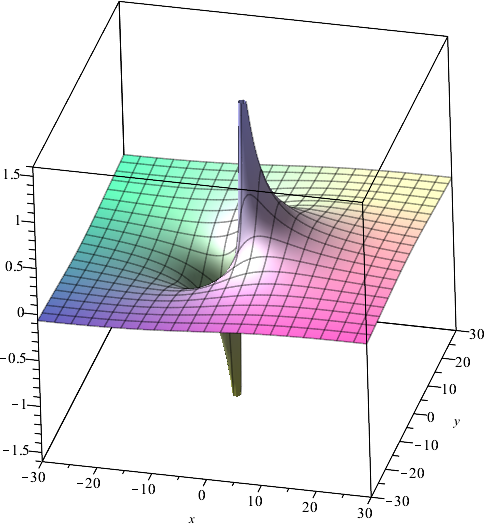
\includegraphics[width=.3\textwidth]{fig/0S1L-1.png}
}
\subfigure[\refeqn{0S1L-2}对应的解 \label{fig-0s1l-2}]{
    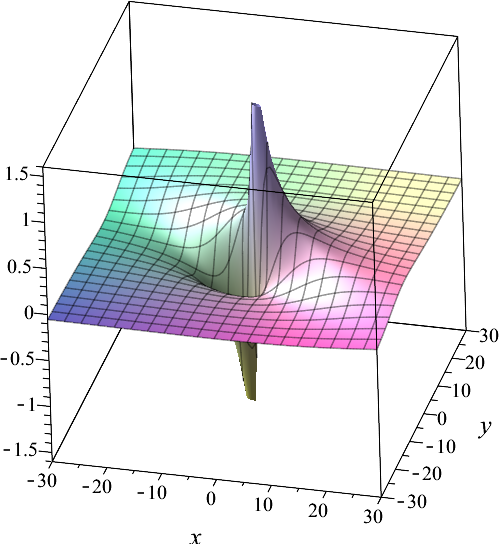
\includegraphics[width=.3\textwidth]{fig/0S1L-2.png}
}
\subfigure[\refeqn{0S1L-3}对应的解 \label{fig-0s1l-3}]{
    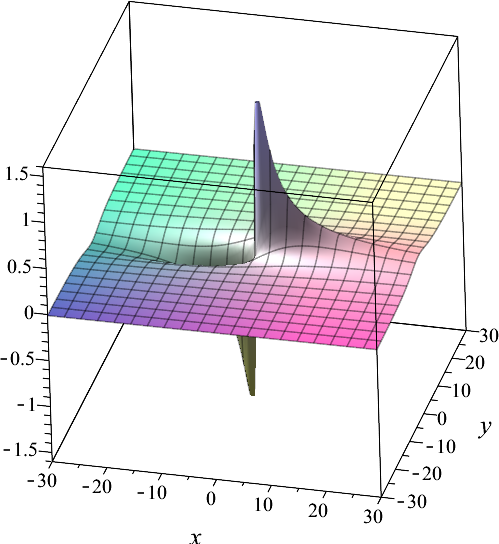
\includegraphics[width=.3\textwidth]{fig/0S1L-3.png}
}
\caption{(3+1)JM 方程的 0S-1L 解}
\end{figure}

综上, 我们已经展示了使用 NS1L 进行求解的一般流程. 

此外, 因为我们以lump解为例进行了求解, 而 TwSolver 也能求 lump 解, 于是我们就来探索一下两种方式得到的解有什么不同. 

由\reftab{verify}可知, (3+1)YTSF方程在$\PS=\bbrace{1,3}$时能通过 TwSolver 得到 lump 解. 调用
\begin{verbatim}
TwSolver:-twsolve(eq,{1,3},PL=[a,b,c,d])
\end{verbatim}
并对计算结果进行代换
\begin{equation}
    b_{1,RE}=\beta,b_{1,IM}=\gamma,c=\delta,
\end{equation}
可以得到lump解
\begin{equation}
    f=\sbrace{x+\beta y + \delta z+ \frac{3\alpha (\beta^2-\gamma^2)}{4}t}^2+\sbrace{\gamma y+\frac{3\alpha \beta \gamma}{2}t}^2-\frac{\delta}{\alpha \gamma^2}. \label{0S1L-3}
\end{equation}
取\verb|[x=-30..30,y=-30..30,alpha=1,t=0,z=0,beta=1/2,gamma=4]|进行绘图, 可以得到\reffig{fig-0s1l-3}. 

经过计算, 我们发现, 当
\begin{equation}
\left\{ 
\begin{array}{l}
p_{11}=\sqrt{1-p_{12}^2},
p_{22}=\beta p_{12}+\gamma p_{11},
p_{21}=\frac{p_{12}(p_{22}-\beta)}{p_{11}},  
p_{32}=\delta p_{12},p_{51}=p_{52}=0
\end{array}
\right\}
\end{equation}
时, \refeqn{0S1L-1}所对应的解能够转化为\refeqn{0S1L-3}. 也就是说, 直接代数方法得到的 lump 解比简单 Hirota 方法得到的解更加具有一般性. 

\subsection{直接求解与继承求解}

接下来, 我们将求解(3+1)YTSF方程的 1S-1L 解. 按照之前的步骤, 我们调用如下代码进行求解. 
\begin{verbatim}
sh:=gen_eq(eq,1,p,q);
ph:=sh:-get_solver(use_parallel);
sols:=ph:-agsolve(5);
sols:=sh:-filter_sol(sols);
\end{verbatim}

在求解时, 我们得到了一个具有16个变量和120个方程的代数方程组. 在求解时, 我们开启了并行加速. 对于这120个方程, 在10秒左右就得到了3个不同的相互作用解. 我们称这种求解方法为\emph{直接求解}.

事实上, 因为在我们假设形式中 1S-1L 解包含了 0S-1L 解, 所以我们也可以将 0S-1L 解为初始解进行求解. 这种方法被称为\emph{继承求解}. 继承求解的调用方式为
\begin{verbatim}
sh:=gen_eq(eq,1,p,q);
ph:=sh:-get_solver(use_parallel);
ph:-set_init_sols(sols0);
sols:=ph:-agsolve(5);
sols:=sh:-filter_sol(sols);
\end{verbatim}
其中, \cd{sols0}表示之前求得的两个 0S-1L 解. 继承求解的关键命令就是在求解开始前, 调用\cd{set\_init\_sols}函数来设置初始解. 按照上述方法进行求解, 在5秒左右获得了3个不同的相互作用解. 经过验证, 这3个解和继承求解的3个解是等价的.

我们可以在\reffig{sb1}中对比直接求解和继承求解的分支图. 在直接求解时, 经历了5轮求解得到3个解, 期间一共计算了14个解. 在继承求解时, 经历4轮求解得到了3个解, 期间一共计算了11个解. 显然继承求解的分支比直接求解更少. 不管是直接求解还是继承求解, 它们都迅速地将方程数量从120降至16, 这就是 PGSolve 能够迅速求解大规模方程的主要原因. 此外, 在\reffig{sb1-d}中还能看到一个绿色的箭头, 这表示10号解等价于7号解, 在求解过程中将 10 号解从 UNSOLVED 中删除, 可以避免重复求解, 减少运行时间. 

\begin{figure}[htbp]
\centering
\subfigure[直接求解的分支图 \label{sb1-d}]{
    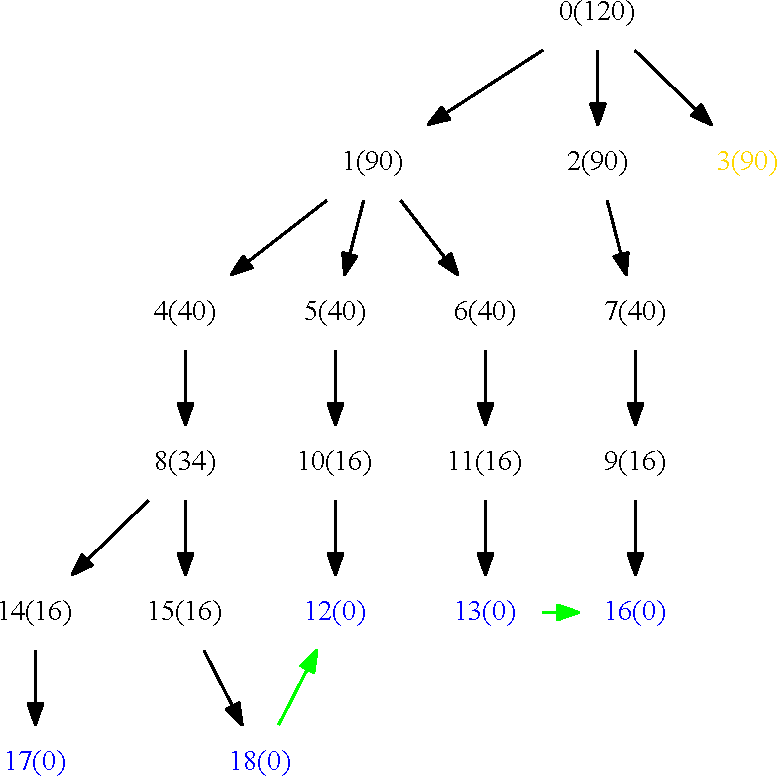
\includegraphics[width=.5\textwidth]{fig/1S1L-dir.pdf}
}
\hfill
\subfigure[继承求解的分支图 \label{sb1-e}]{
    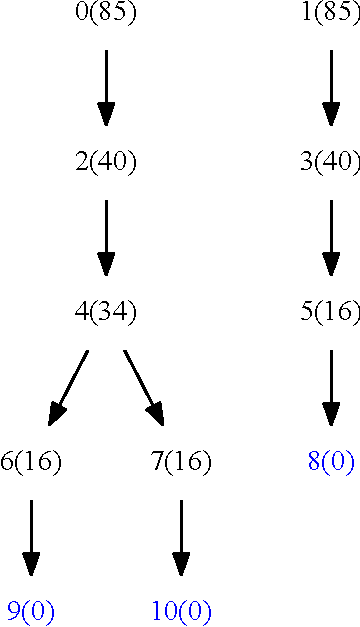
\includegraphics[width=.35\textwidth]{fig/1S1L-ext.pdf}
}
\caption{1S-1L的直接求解与继承求解对比图} \label{sb1}
\end{figure}

为了简化解的表示, 同时也为了能够和\citett{zhangYTSF}中的结果进行对比, 我们取解的假设形式为
\begin{equation}
\begin{split}
    f&=(a_1 x+a_2 y+a_3 z+ a_4 t +a_5)^2+(a_6 x+a_7 y+a_8 z+ a_9 t +a_{10})^2 \\
    &+b+k \exp(k_1 x + k_2 y +k_3 z+ k_4 t).
\end{split}
\end{equation}

NS1L得到的三个解为
\begin{eqnarray}
\def\arraystretch{1.2}
\left\{
\begin{array}{l}
b=\frac{\left( {{{a}_{1}}}^{2}+{{{a}_{6}}}^{2}\right) }{{{{k}_{1}}}^{2}},
{{a}_{2}}=\frac{\left( {{{a}_{1}}}^{2}\,{{k}_{2}}+{{{a}_{6}}}^{2}\,{{k}_{2}}-{{a}_{6}}\,{{k}_{1}}\,{{a}_{7}}\right) }{{{a}_{1}}\,{{k}_{1}}},
{{a}_{3}}=-\frac{\alpha\,\left( {{a}_{6}}\,{{k}_{2}}-{{a}_{7}}\,{{k}_{1}}\right) ^{2}}{{{a}_{1}}\,{{{k}_{1}}}^{4}},\\
{{a}_{4}}=\frac{3\,\alpha\,\left( {{{a}_{1}}}^{2}\,{{{k}_{2}}}^{2}+{{{a}_{6}}}^{2}\,{{{k}_{2}}}^{2}-{{{k}_{1}}}^{2}\,{{{a}_{7}}}^{2}\right) }{4\,{{{k}_{1}}}^{2}\,{{a}_{1}}},
{{a}_{8}}=-\frac{{{a}_{6}}\,\alpha\,\left( {{a}_{6}}\,{{k}_{2}}-{{a}_{7}}\,{{k}_{1}}\right) ^{2}}{{{{a}_{1}}}^{2}\,{{{k}_{1}}}^{4}},\\
{{k}_{3}}=-\frac{\alpha\,\left( {{a}_{6}}\,{{k}_{2}}-{{a}_{7}}\,{{k}_{1}}\right) ^{2}}{{{{a}_{1}}}^{2}\,{{{k}_{1}}}^{3}},
{{k}_{4}}=\frac{\alpha\,\left( 3\,{{{a}_{1}}}^{2}\,{{{k}_{2}}}^{2}-{{{a}_{6}}}^{2}\,{{{k}_{2}}}^{2}+2\,{{a}_{6}}\,{{a}_{7}}\,{{k}_{1}}\,{{k}_{2}}-{{{k}_{1}}}^{2}\,{{{a}_{7}}}^{2}\right) }{4\,{{{a}_{1}}}^{2}\,{{k}_{1}}},\\
{{a}_{9}}=-\frac{3\,\alpha\,\left( {{{a}_{1}}}^{2}\,{{a}_{6}}\,{{{k}_{2}}}^{2}-2\,{{{a}_{1}}}^{2}\,{{a}_{7}}\,{{k}_{1}}\,{{k}_{2}}+{{{a}_{6}}}^{3}\,{{{k}_{2}}}^{2}-2\,{{{a}_{6}}}^{2}\,{{a}_{7}}\,{{k}_{1}}\,{{k}_{2}}+{{a}_{6}}\,{{{a}_{7}}}^{2}\,{{{k}_{1}}}^{2}\right) }{4\,{{{a}_{1}}}^{2}\,{{{k}_{1}}}^{2}}\\
\end{array}
\right\}, \label{1S1L-1}
\end{eqnarray}
\begin{equation}
\def\arraystretch{1.2}
\left\{
\begin{array}{l}  
b=\frac{{{{a}_{2}}}^{2}}{{{{k}_{2}}}^{2}},
{{a}_{3}}=-\frac{\alpha\,{{{a}_{2}}}^{2}\,{{{a}_{7}}}^{2}}{{{{a}_{1}}}^{3}\,{{{k}_{2}}}^{2}},
{{a}_{4}}=\frac{3\,\alpha\,\left( {{{a}_{2}}}^{2}-{{{a}_{7}}}^{2}\right) }{4\,{{a}_{1}}},
{{a}_{6}}=0,
{{a}_{8}}=0,\\
{{a}_{9}}=\frac{3\,\alpha\,{{a}_{2}}\,{{a}_{7}}}{2\,{{a}_{1}}},
{{k}_{1}}=\frac{{{a}_{1}}\,{{k}_{2}}}{{{a}_{2}}},
{{k}_{3}}=-\frac{{{a}_{2}}\,\alpha\,{{{a}_{7}}}^{2}}{{{{a}_{1}}}^{3}\,{{k}_{2}}},
{{k}_{4}}=\frac{\alpha\,{{k}_{2}}\,\left( 3\,{{{a}_{2}}}^{2}-{{{a}_{7}}}^{2}\right) }{4\,{{a}_{1}}\,{{a}_{2}}}
\end{array}
\right\} \label{1S1L-2}
\end{equation}
和
\begin{equation}
\def\arraystretch{1.2}
\left\{
\begin{array}{l}  
b=\frac{{{{a}_{6}}}^{2}}{{{{k}_{1}}}^{2}},
{{a}_{1}}=0,
{{a}_{3}}=0,
{{a}_{4}}=\frac{3\,\alpha\,{{a}_{2}}\,{{k}_{2}}}{2\,{{k}_{1}}},
{{a}_{7}}=\frac{{{a}_{6}}\,{{k}_{2}}}{{{k}_{1}}},
{{a}_{8}}=-\frac{\alpha\,{{{a}_{2}}}^{2}}{{{{k}_{1}}}^{2}\,{{a}_{6}}},\\
{{a}_{9}}=-\frac{3\,\alpha\,\left( {{{a}_{2}}}^{2}\,{{{k}_{1}}}^{2}-{{{a}_{6}}}^{2}\,{{{k}_{2}}}^{2}\right) }{4\,{{{k}_{1}}}^{2}\,{{a}_{6}}},
{{k}_{3}}=-\frac{\alpha\,{{{a}_{2}}}^{2}}{{{k}_{1}}\,{{{a}_{6}}}^{2}},
{{k}_{4}}=-\frac{\alpha\,\left( {{{a}_{2}}}^{2}\,{{{k}_{1}}}^{2}-3\,{{{a}_{6}}}^{2}\,{{{k}_{2}}}^{2}\right) }{4\,{{k}_{1}}\,{{{a}_{6}}}^{2}}
\end{array}
\right\}. \label{1S1L-3}
\end{equation}

经验证发现, \refeqn{0S1L-1}对应的解和\citett{zhangYTSF}中的解是等价的. 也就是说, NS1L得到的解更加全面. 

对于上述三个解, 取$a_2=2,k=1/3,t=0,z=0$, 其它参数取1, 可以得到如\reffig{fig-1S1L}所示的三个解. 

\begin{figure}[htbp]
\centering
\subfigure[\refeqn{1S1L-1}对应的解]{
    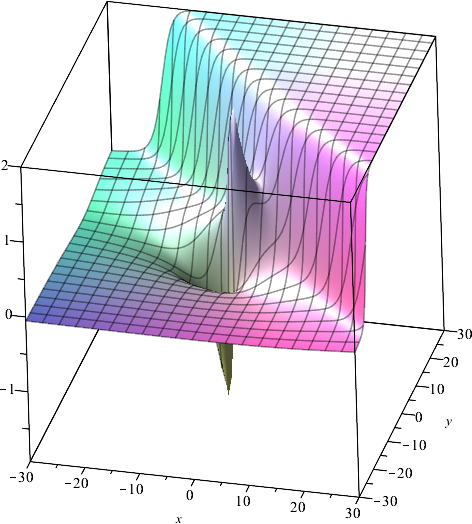
\includegraphics[width=.3\textwidth]{fig/1S1L-1.png}
}
\subfigure[\refeqn{1S1L-2}对应的解]{
    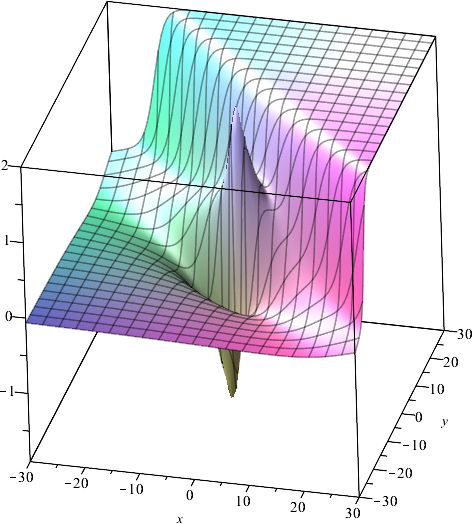
\includegraphics[width=.3\textwidth]{fig/1S1L-2.png}
}
\subfigure[\refeqn{1S1L-3}对应的解]{
    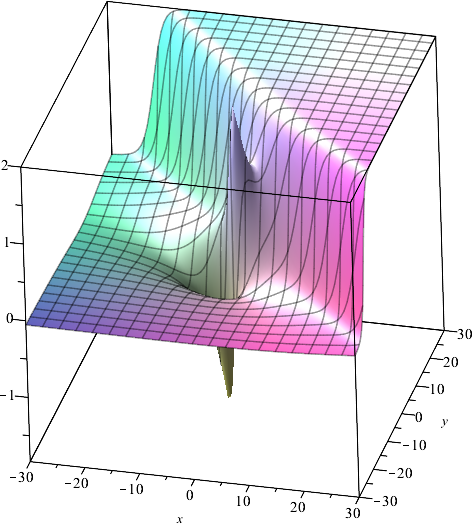
\includegraphics[width=.3\textwidth]{fig/1S1L-3.png}
}
\caption{(3+1)JM 方程的 1S-1L 解} \label{fig-1S1L}
\end{figure}

从\reffig{fig-1S1L}可以看出, 在相同的参数条件下, 3个解存在细微的差别, 但它们都是一个扭状孤子和lump解相互作用的结果. 

最后, 我们来求解 2S-1L 解. 通过
\begin{verbatim}
sh:=gen_eq(eq,2,p,q);
ph:=sh:-get_solver(use_parallel);
\end{verbatim}
可以得到一个具有22个变量和324个方程的方程组. 

采用继承求解的方式, 我们在8核CPU (Intel Core i7-7700K @ 4.2GHz) 的硬件条件下, 用时 36 秒, 解得3个解. 该过程的求解分支图如\reffig{sb2-e}所示. 从图中可以看出, 以 1S-1L 的三个解为初始解, 方程的个数迅速地从202个降为7个, 在第5轮求解中得到了3个解. 

\begin{figure}[htbp]
\centering
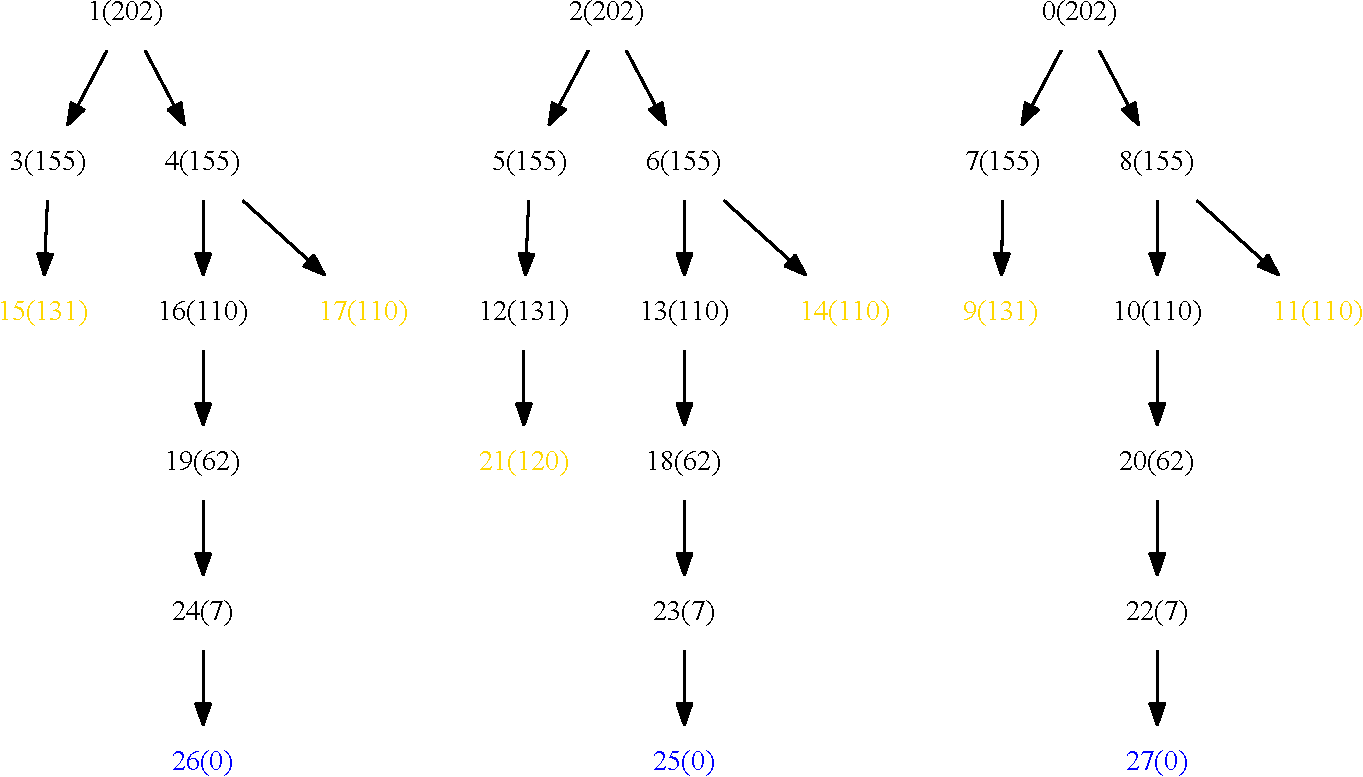
\includegraphics[width=\textwidth]{fig/2S1L-ext.pdf}
\caption{2S-1L 继承求解的分支图}\label{sb2-e}
\end{figure}

而采用直接求解的方式, 设置单步最大时长为100,秒, 最终运行时间430秒, 得到了5个解, 其求解分支图如\reffig{sb2-d}所示. 可以看出求解的分支明显增多, 求解的增根也明显增多, 还出现了一个求解超时的解.  

\begin{figure}[htbp]
\centering
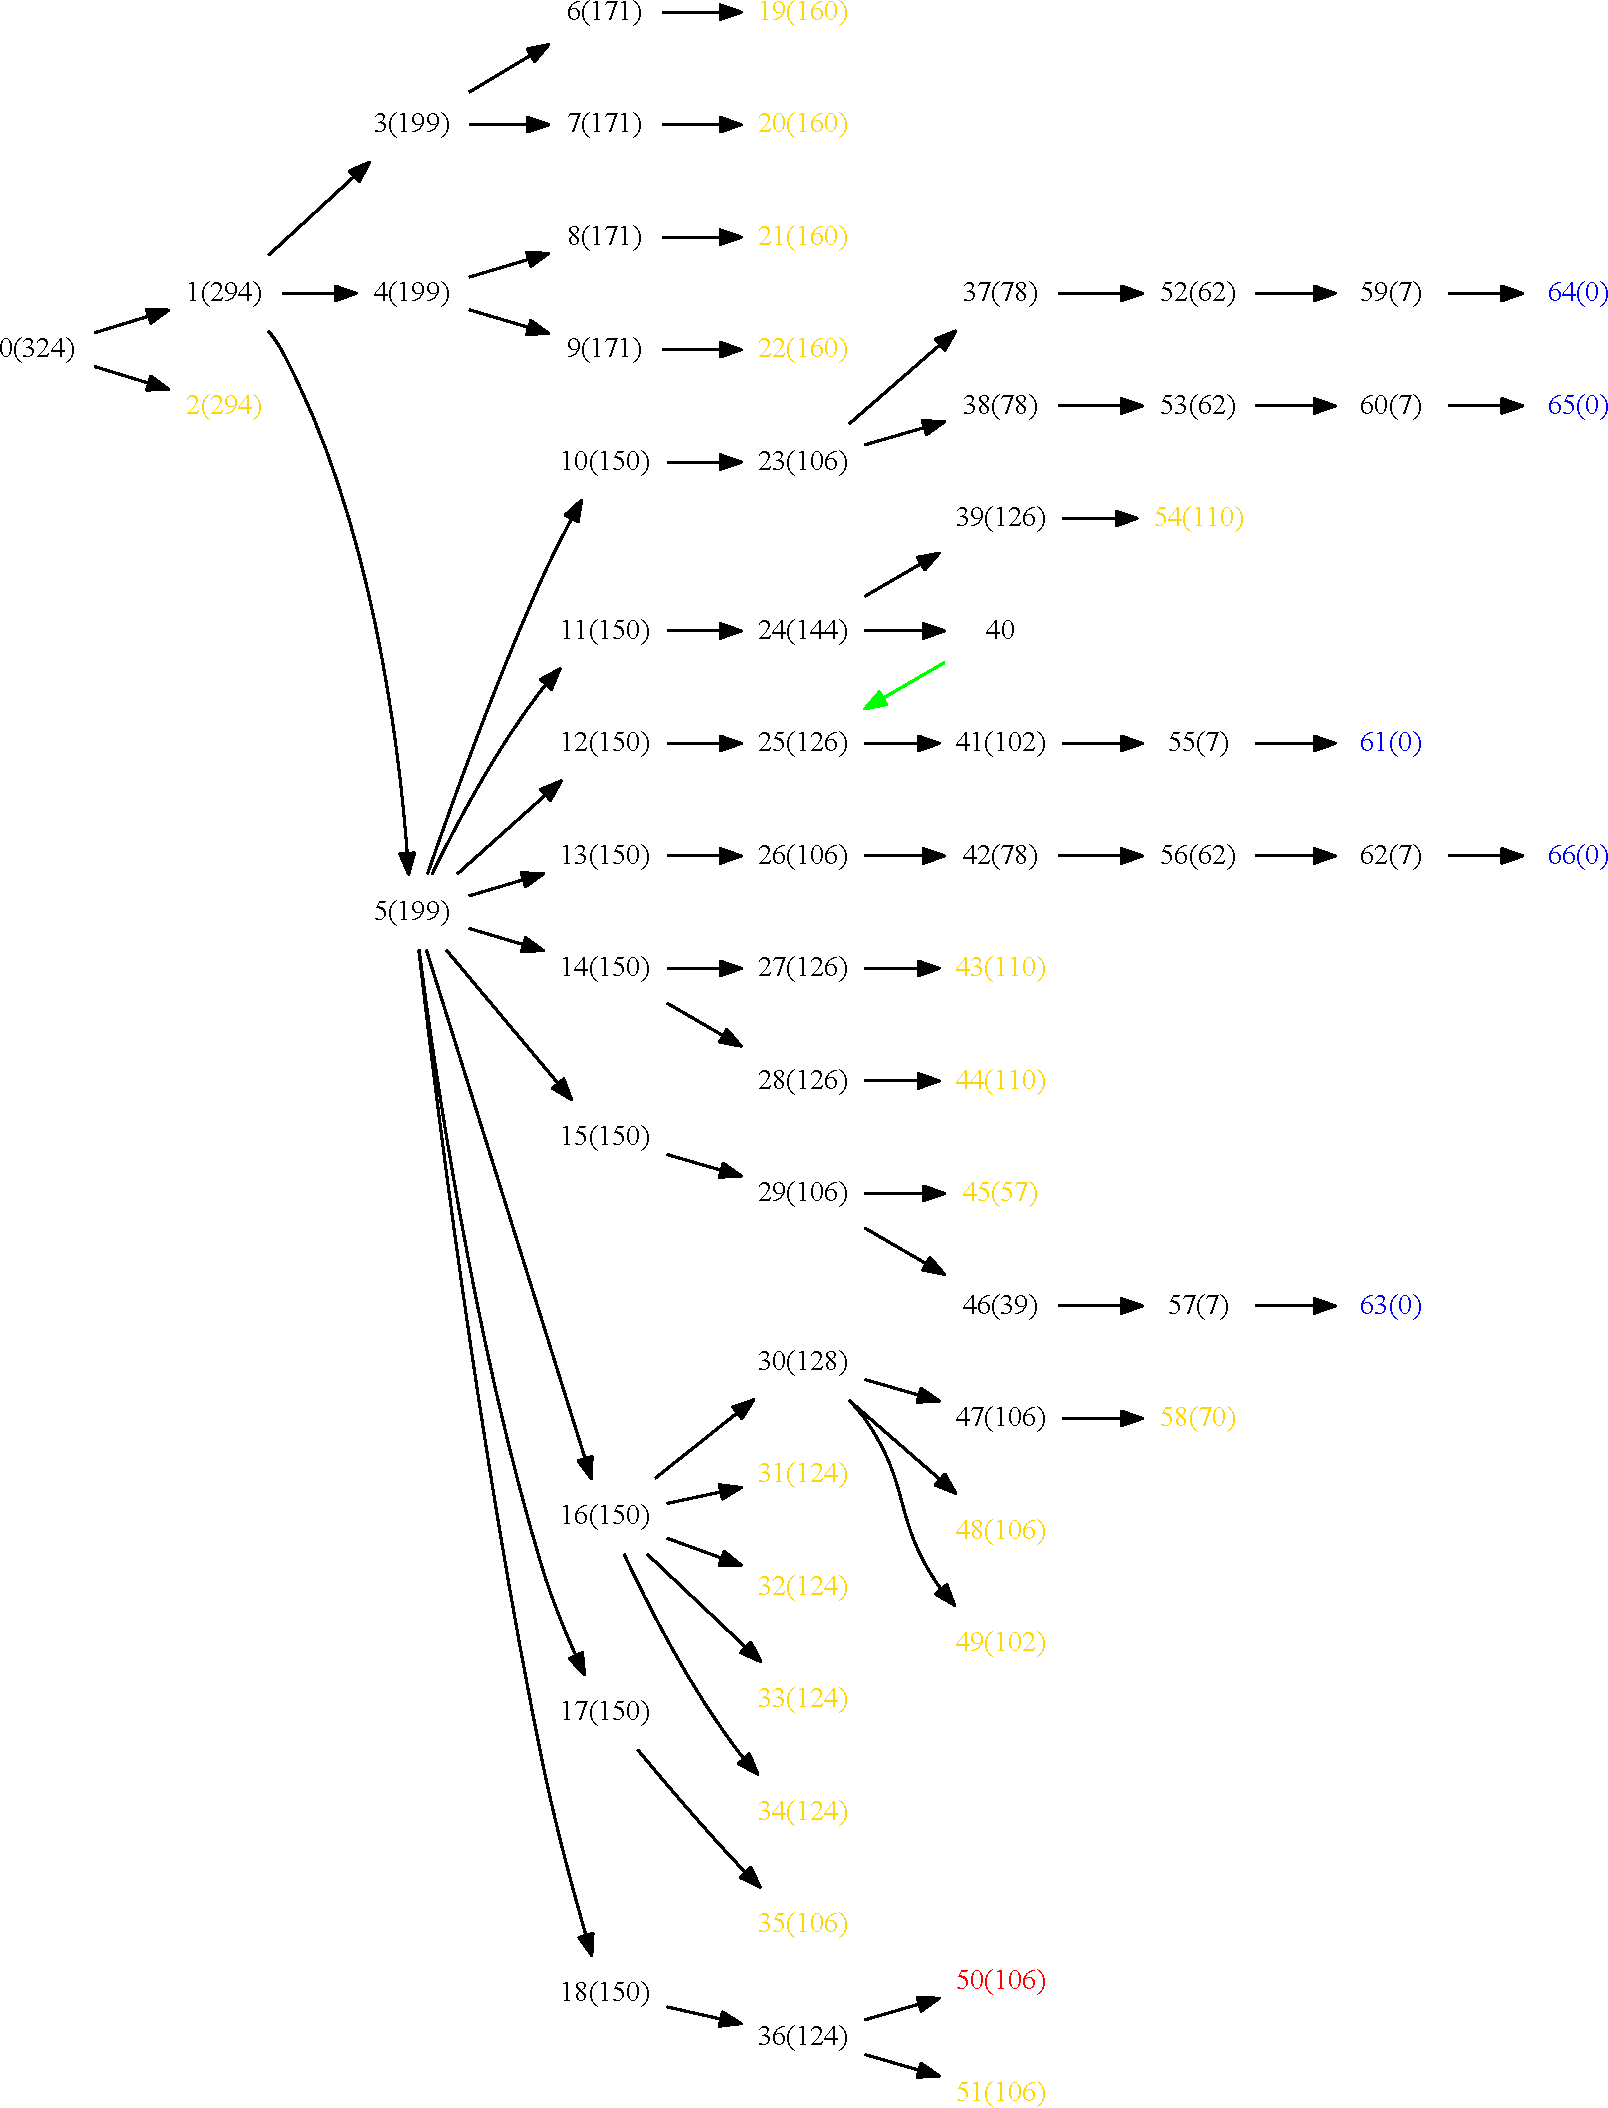
\includegraphics[width=\textwidth]{fig/2S1L-dir-number.pdf}
\caption{2S-1L 直接求解的分支图}\label{sb2-d}
\end{figure}

两种解法有两个共同的解
\begin{equation}
\def\arraystretch{1.2}
\left\{
\begin{array}{l}
{{p}_{11}}=0,
{{p}_{13}}=-{{p}_{14}},
{{p}_{22}}=\frac{{{p}_{12}}\,{{p}_{24}}}{{{p}_{14}}},
{{p}_{23}}=-{{p}_{24}},
{{p}_{31}}=0,\\
{{p}_{32}}=-\frac{\alpha\,{{{p}_{21}}}^{2}}{{{{p}_{14}}}^{2}\,{{p}_{12}}},
{{p}_{33}}=\frac{\alpha\,{{{p}_{21}}}^{2}}{{{{p}_{12}}}^{2}\,{{p}_{14}}},
{{p}_{34}}=-\frac{\alpha\,{{{p}_{21}}}^{2}}{{{{p}_{12}}}^{2}\,{{p}_{14}}},
{{p}_{41}}=\frac{3\,\alpha\,{{p}_{21}}\,{{p}_{24}}}{2\,{{p}_{14}}},\\ 
{{p}_{42}}=\frac{3\,\alpha\,\left( {{{p}_{12}}}^{2}\,{{{p}_{24}}}^{2}-{{{p}_{14}}}^{2}\,{{{p}_{21}}}^{2}\right) }{4\,{{{p}_{14}}}^{2}\,{{p}_{12}}},
{{p}_{43}}=-\frac{\left( 3\,{{{p}_{12}}}^{2}\,{{{p}_{24}}}^{2}-{{{p}_{14}}}^{2}\,{{{p}_{21}}}^{2}\right) \,\alpha}{4\,{{{p}_{12}}}^{2}\,{{p}_{14}}},\\
{{p}_{44}}=\frac{\left( 3\,{{{p}_{12}}}^{2}\,{{{p}_{24}}}^{2}-{{{p}_{14}}}^{2}\,{{{p}_{21}}}^{2}\right) \,\alpha}{4\,{{{p}_{12}}}^{2}\,{{p}_{14}}},
{{q}_{1}}=\frac{{{{p}_{12}}}^{2}}{{{{p}_{14}}}^{2}},
{{q}_{4}}=\frac{{{{p}_{14}}}^{2}\,{{q}_{2}}\,{{q}_{3}}}{{{{p}_{12}}}^{2}}
\end{array}
\right\}
\end{equation}
和
\begin{equation}
\def\arraystretch{1.2}
\left\{
\begin{array}{l}
{{p}_{12}}=0,
{{p}_{13}}=-\frac{{{p}_{11}}\,{{p}_{24}}}{{{p}_{21}}},
{{p}_{14}}=\frac{{{p}_{11}}\,{{p}_{24}}}{{{p}_{21}}},
{{p}_{23}}=-{{p}_{24}},
{{p}_{31}}=-\frac{\alpha\,{{{p}_{22}}}^{2}\,{{{p}_{21}}}^{2}}{{{{p}_{24}}}^{2}\,{{{p}_{11}}}^{3}},
{{p}_{32}}=0,\\ 
{{p}_{33}}=\frac{{{p}_{21}}\,\alpha\,{{{p}_{22}}}^{2}}{{{{p}_{11}}}^{3}\,{{p}_{24}}},
{{p}_{34}}=-\frac{{{p}_{21}}\,\alpha\,{{{p}_{22}}}^{2}}{{{{p}_{11}}}^{3}\,{{p}_{24}}},
{{p}_{41}}=\frac{3\,\alpha\,\left( {{{p}_{21}}}^{2}-{{{p}_{22}}}^{2}\right) }{4\,{{p}_{11}}},
{{p}_{42}}=\frac{3\,\alpha\,{{p}_{21}}\,{{p}_{22}}}{2\,{{p}_{11}}},\\ 
{{p}_{43}}=-\frac{{{p}_{24}}\,\left( 3\,{{{p}_{21}}}^{2}-{{{p}_{22}}}^{2}\right) \,\alpha}{4\,{{p}_{11}}\,{{p}_{21}}},
{{p}_{44}}=\frac{{{p}_{24}}\,\left( 3\,{{{p}_{21}}}^{2}-{{{p}_{22}}}^{2}\right) \,\alpha}{4\,{{p}_{11}}\,{{p}_{21}}},
{{q}_{1}}=\frac{{{{p}_{21}}}^{2}}{{{{p}_{24}}}^{2}},
{{q}_{4}}=\frac{{{{p}_{24}}}^{2}\,{{q}_{2}}\,{{q}_{3}}}{{{{p}_{21}}}^{2}}
\end{array}
\right\} . 
\end{equation}

直接求解特有的三个解为
\begin{equation}
\def\arraystretch{1.2}
\left\{
\begin{array}{l}
{{p}_{11}}=-\frac{3\,\alpha\,{{{p}_{22}}}^{2}\,{{p}_{41}}}{\left( 4\,{{{p}_{41}}}^{2}+4\,{{{p}_{42}}}^{2}\right) },
{{p}_{12}}=\frac{3\,\alpha\,{{{p}_{22}}}^{2}\,{{p}_{42}}}{\left( 4\,{{{p}_{41}}}^{2}+4\,{{{p}_{42}}}^{2}\right) },
{{p}_{13}}=-\frac{3\,\alpha\,{{p}_{22}}\,{{p}_{24}}}{4\,{{p}_{42}}},
{{p}_{14}}=\frac{3\,\alpha\,{{p}_{22}}\,{{p}_{24}}}{4\,{{p}_{42}}},\\ 
{{p}_{23}}=-{{p}_{24}},
{{p}_{31}}=\frac{64\,{{{p}_{41}}}^{3}\,{{{p}_{42}}}^{2}}{27\,{\alpha}^{2}\,{{{p}_{22}}}^{2}\,{{{p}_{24}}}^{2}\,\left( {{{p}_{41}}}^{2}+{{{p}_{42}}}^{2}\right) },
{{p}_{32}}=-\frac{64\,{{{p}_{41}}}^{2}\,{{{p}_{42}}}^{3}}{27\,{\alpha}^{2}\,{{{p}_{22}}}^{2}\,{{{p}_{24}}}^{2}\,\left( {{{p}_{41}}}^{2}+{{{p}_{42}}}^{2}\right) },\\ 
{{p}_{21}}=0,
{{p}_{33}}=\frac{64\,{{{p}_{41}}}^{2}\,{{p}_{42}}}{27\,{\alpha}^{2}\,{{p}_{24}}\,{{{p}_{22}}}^{3}},
{{p}_{34}}=-\frac{64\,{{{p}_{41}}}^{2}\,{{p}_{42}}}{27\,{\alpha}^{2}\,{{p}_{24}}\,{{{p}_{22}}}^{3}},
{{p}_{43}}=\frac{{{p}_{24}}\,\left( {{{p}_{41}}}^{2}-3\,{{{p}_{42}}}^{2}\right) }{3\,{{p}_{42}}\,{{p}_{22}}},\\ 
{{p}_{44}}=-\frac{{{p}_{24}}\,\left( {{{p}_{41}}}^{2}-3\,{{{p}_{42}}}^{2}\right) }{3\,{{p}_{42}}\,{{p}_{22}}},
{{q}_{1}}=\frac{{{{p}_{22}}}^{2}\,{{{p}_{42}}}^{2}}{{{{p}_{24}}}^{2}\,\left( {{{p}_{41}}}^{2}+{{{p}_{42}}}^{2}\right) },
{{q}_{4}}=\frac{{{q}_{2}}\,{{q}_{3}}\,{{{p}_{24}}}^{2}\,\left( {{{p}_{41}}}^{2}+{{{p}_{42}}}^{2}\right) }{{{{p}_{22}}}^{2}\,{{{p}_{42}}}^{2}}
\end{array}
\right\} ,
\end{equation}
\begin{equation}
\def\arraystretch{1.2}
\left\{
\begin{array}{l}
{{p}_{11}}=\frac{{{p}_{14}}\,{{p}_{21}}}{{{p}_{24}}},
% {{p}_{12}}=0,
% {{p}_{52}}=0,
% {{p}_{32}}=0,
p_{12}=p_{32}=p_{52}=0,
{{p}_{13}}=-{{p}_{14}},
{{p}_{23}}=-{{p}_{24}},
{{p}_{31}}=-\frac{{{{p}_{22}}}^{2}\,{{p}_{24}}\,\alpha}{{{{p}_{14}}}^{3}\,{{p}_{21}}},\\ 
{{p}_{33}}=\frac{{{{p}_{22}}}^{2}\,{{{p}_{24}}}^{2}\,\alpha}{{{{p}_{21}}}^{2}\,{{{p}_{14}}}^{3}},
{{p}_{34}}=-\frac{{{{p}_{22}}}^{2}\,{{{p}_{24}}}^{2}\,\alpha}{{{{p}_{21}}}^{2}\,{{{p}_{14}}}^{3}},
{{p}_{41}}=\frac{3\,{{p}_{24}}\,\alpha\,\left( {{{p}_{21}}}^{2}-{{{p}_{22}}}^{2}\right) }{4\,{{p}_{14}}\,{{p}_{21}}},
{{p}_{42}}=\frac{3\,\alpha\,{{p}_{22}}\,{{p}_{24}}}{2\,{{p}_{14}}},\\ 
{{p}_{43}}=-\frac{{{{p}_{24}}}^{2}\,\left( 3\,{{{p}_{21}}}^{2}-{{{p}_{22}}}^{2}\right) \,\alpha}{4\,{{{p}_{21}}}^{2}\,{{p}_{14}}},
{{p}_{44}}=\frac{{{{p}_{24}}}^{2}\,\left( 3\,{{{p}_{21}}}^{2}-{{{p}_{22}}}^{2}\right) \,\alpha}{4\,{{{p}_{21}}}^{2}\,{{p}_{14}}},
{{q}_{1}}=\frac{{{{p}_{21}}}^{2}}{{{{p}_{24}}}^{2}},
{{q}_{4}}=\frac{{{{p}_{24}}}^{2}\,{{q}_{2}}\,{{q}_{3}}}{{{{p}_{21}}}^{2}},
\end{array}
\right\}
\end{equation}
和
\begin{equation}
\def\arraystretch{1.2}
\left\{
\begin{array}{l}
{{p}_{11}}=\frac{3\,{{p}_{14}}\,\left( 3\,\alpha\,{{{p}_{21}}}^{2}\,{{p}_{24}}-3\,\alpha\,{{{p}_{22}}}^{2}\,{{p}_{24}}+4\,{{p}_{14}}\,{{p}_{22}}\,{{p}_{42}}\right) \,{{p}_{21}}\,\alpha}{\left( 9\,{\alpha}^{2}\,{{{p}_{21}}}^{2}\,{{{p}_{24}}}^{2}+9\,{\alpha}^{2}\,{{{p}_{22}}}^{2}\,{{{p}_{24}}}^{2}-24\,\alpha\,{{p}_{14}}\,{{p}_{22}}\,{{p}_{24}}\,{{p}_{42}}+16\,{{{p}_{14}}}^{2}\,{{{p}_{42}}}^{2}\right) },\\ 
{{p}_{12}}=\frac{6\,{{p}_{14}}\,\left( 3\,\alpha\,{{p}_{22}}\,{{p}_{24}}-2\,{{p}_{14}}\,{{p}_{42}}\right) \,{{{p}_{21}}}^{2}\,\alpha}{\left( 9\,{\alpha}^{2}\,{{{p}_{21}}}^{2}\,{{{p}_{24}}}^{2}+9\,{\alpha}^{2}\,{{{p}_{22}}}^{2}\,{{{p}_{24}}}^{2}-24\,\alpha\,{{p}_{14}}\,{{p}_{22}}\,{{p}_{24}}\,{{p}_{42}}+16\,{{{p}_{14}}}^{2}\,{{{p}_{42}}}^{2}\right) },\\
{{p}_{31}}=-\frac{\left( 3\,\alpha\,{{p}_{22}}\,{{p}_{24}}-4\,{{p}_{14}}\,{{p}_{42}}\right) ^{2}\,\left( 3\,\alpha\,{{{p}_{21}}}^{2}\,{{p}_{24}}-3\,\alpha\,{{{p}_{22}}}^{2}\,{{p}_{24}}+4\,{{p}_{14}}\,{{p}_{22}}\,{{p}_{42}}\right) }{3\,{{{p}_{14}}}^{3}\,\left( 9\,{\alpha}^{2}\,{{{p}_{21}}}^{2}\,{{{p}_{24}}}^{2}+9\,{\alpha}^{2}\,{{{p}_{22}}}^{2}\,{{{p}_{24}}}^{2}-24\,\alpha\,{{p}_{14}}\,{{p}_{22}}\,{{p}_{24}}\,{{p}_{42}}+16\,{{{p}_{14}}}^{2}\,{{{p}_{42}}}^{2}\right) \,{{p}_{21}}},\\
{{p}_{32}}=-\frac{2\,\left( 3\,\alpha\,{{p}_{22}}\,{{p}_{24}}-2\,{{p}_{14}}\,{{p}_{42}}\right) \,\left( 3\,\alpha\,{{p}_{22}}\,{{p}_{24}}-4\,{{p}_{14}}\,{{p}_{42}}\right) ^{2}}{3\,{{{p}_{14}}}^{3}\,\left( 9\,{\alpha}^{2}\,{{{p}_{21}}}^{2}\,{{{p}_{24}}}^{2}+9\,{\alpha}^{2}\,{{{p}_{22}}}^{2}\,{{{p}_{24}}}^{2}-24\,\alpha\,{{p}_{14}}\,{{p}_{22}}\,{{p}_{24}}\,{{p}_{42}}+16\,{{{p}_{14}}}^{2}\,{{{p}_{42}}}^{2}\right) },\\ 
{{p}_{33}}=\frac{\left( 3\,\alpha\,{{p}_{22}}\,{{p}_{24}}-4\,{{p}_{14}}\,{{p}_{42}}\right) ^{2}}{9\,{{{p}_{21}}}^{2}\,\alpha\,{{{p}_{14}}}^{3}},
{{p}_{34}}=-\frac{\left( 3\,\alpha\,{{p}_{22}}\,{{p}_{24}}-4\,{{p}_{14}}\,{{p}_{42}}\right) ^{2}}{9\,{{{p}_{21}}}^{2}\,\alpha\,{{{p}_{14}}}^{3}},\\ 
{{p}_{41}}=\frac{\left( 3\,\alpha\,{{{p}_{21}}}^{2}\,{{p}_{24}}+3\,\alpha\,{{{p}_{22}}}^{2}\,{{p}_{24}}-4\,{{p}_{14}}\,{{p}_{22}}\,{{p}_{42}}\right) }{4\,{{p}_{14}}\,{{p}_{21}}},
{{p}_{13}}=-{{p}_{14}},
{{p}_{23}}=-{{p}_{24}},\\ 
{{p}_{43}}=\frac{\left( -27\,{\alpha}^{2}\,{{{p}_{21}}}^{2}\,{{{p}_{24}}}^{2}+9\,{\alpha}^{2}\,{{{p}_{22}}}^{2}\,{{{p}_{24}}}^{2}-24\,\alpha\,{{p}_{14}}\,{{p}_{22}}\,{{p}_{24}}\,{{p}_{42}}+16\,{{{p}_{14}}}^{2}\,{{{p}_{42}}}^{2}\right) }{36\,{{{p}_{21}}}^{2}\,\alpha\,{{p}_{14}}},\\ 
{{p}_{44}}=\frac{\left( 27\,{\alpha}^{2}\,{{{p}_{21}}}^{2}\,{{{p}_{24}}}^{2}-9\,{\alpha}^{2}\,{{{p}_{22}}}^{2}\,{{{p}_{24}}}^{2}+24\,\alpha\,{{p}_{14}}\,{{p}_{22}}\,{{p}_{24}}\,{{p}_{42}}-16\,{{{p}_{14}}}^{2}\,{{{p}_{42}}}^{2}\right) }{36\,{{{p}_{21}}}^{2}\,\alpha\,{{p}_{14}}},\\ 
{{q}_{1}}=\frac{9\,{\alpha}^{2}\,{{{p}_{21}}}^{2}\,\left( {{{p}_{21}}}^{2}+{{{p}_{22}}}^{2}\right) }{\left( 9\,{\alpha}^{2}\,{{{p}_{21}}}^{2}\,{{{p}_{24}}}^{2}+9\,{\alpha}^{2}\,{{{p}_{22}}}^{2}\,{{{p}_{24}}}^{2}-24\,\alpha\,{{p}_{14}}\,{{p}_{22}}\,{{p}_{24}}\,{{p}_{42}}+16\,{{{p}_{14}}}^{2}\,{{{p}_{42}}}^{2}\right) },\\ 
{{q}_{4}}=\frac{{{q}_{2}}\,{{q}_{3}}\,\left( 9\,{\alpha}^{2}\,{{{p}_{21}}}^{2}\,{{{p}_{24}}}^{2}+9\,{\alpha}^{2}\,{{{p}_{22}}}^{2}\,{{{p}_{24}}}^{2}-24\,\alpha\,{{p}_{14}}\,{{p}_{22}}\,{{p}_{24}}\,{{p}_{42}}+16\,{{{p}_{14}}}^{2}\,{{{p}_{42}}}^{2}\right) }{9\,{\alpha}^{2}\,{{{p}_{21}}}^{2}\,\left( {{{p}_{21}}}^{2}+{{{p}_{22}}}^{2}\right) }
\end{array}
\right\} . \label{2S1L-eq}
\end{equation} 

继承求解特有的解为 
\begin{equation}
\def\arraystretch{1.2}
\left\{
\begin{array}{l}
{{p}_{13}}=-{{p}_{14}},
{{p}_{21}}=\frac{\left( {{{p}_{11}}}^{2}\,{{p}_{24}}+{{{p}_{12}}}^{2}\,{{p}_{24}}-{{p}_{12}}\,{{p}_{14}}\,{{p}_{22}}\right) }{{{p}_{11}}\,{{p}_{14}}},
{{p}_{23}}=-{{p}_{24}},\\
{{p}_{32}}=-\frac{{{p}_{12}}\,\alpha\,\left( {{p}_{12}}\,{{p}_{24}}-{{p}_{14}}\,{{p}_{22}}\right) ^{2}}{{{{p}_{11}}}^{2}\,{{{p}_{14}}}^{4}},
{{p}_{33}}=\frac{\alpha\,\left( {{p}_{12}}\,{{p}_{24}}-{{p}_{14}}\,{{p}_{22}}\right) ^{2}}{{{{p}_{11}}}^{2}\,{{{p}_{14}}}^{3}},
{{p}_{34}}=-\frac{\alpha\,\left( {{p}_{12}}\,{{p}_{24}}-{{p}_{14}}\,{{p}_{22}}\right) ^{2}}{{{{p}_{11}}}^{2}\,{{{p}_{14}}}^{3}},\\
{{p}_{41}}=\frac{3\,\alpha\,\left( {{{p}_{11}}}^{2}\,{{{p}_{24}}}^{2}+{{{p}_{12}}}^{2}\,{{{p}_{24}}}^{2}-{{{p}_{14}}}^{2}\,{{{p}_{22}}}^{2}\right) }{4\,{{p}_{11}}\,{{{p}_{14}}}^{2}},
{{p}_{31}}=-\frac{\alpha\,\left( {{p}_{12}}\,{{p}_{24}}-{{p}_{14}}\,{{p}_{22}}\right) ^{2}}{{{p}_{11}}\,{{{p}_{14}}}^{4}},\\
{{p}_{42}}=-\frac{3\,\alpha\,\left( {{{p}_{11}}}^{2}\,{{p}_{12}}\,{{{p}_{24}}}^{2}-2\,{{{p}_{11}}}^{2}\,{{p}_{14}}\,{{p}_{22}}\,{{p}_{24}}+{{{p}_{12}}}^{3}\,{{{p}_{24}}}^{2}-2\,{{{p}_{12}}}^{2}\,{{p}_{14}}\,{{p}_{22}}\,{{p}_{24}}+{{p}_{12}}\,{{{p}_{14}}}^{2}\,{{{p}_{22}}}^{2}\right) }{4\,{{{p}_{11}}}^{2}\,{{{p}_{14}}}^{2}},\\ 
{{p}_{43}}=-\frac{\alpha\,\left( 3\,{{{p}_{11}}}^{2}\,{{{p}_{24}}}^{2}-{{{p}_{12}}}^{2}\,{{{p}_{24}}}^{2}+2\,{{p}_{12}}\,{{p}_{14}}\,{{p}_{22}}\,{{p}_{24}}-{{{p}_{14}}}^{2}\,{{{p}_{22}}}^{2}\right) }{4\,{{{p}_{11}}}^{2}\,{{p}_{14}}},
{{q}_{1}}=\frac{\left( {{{p}_{11}}}^{2}+{{{p}_{12}}}^{2}\right) }{{{{p}_{14}}}^{2}},\\ 
{{p}_{44}}=\frac{\alpha\,\left( 3\,{{{p}_{11}}}^{2}\,{{{p}_{24}}}^{2}-{{{p}_{12}}}^{2}\,{{{p}_{24}}}^{2}+2\,{{p}_{12}}\,{{p}_{14}}\,{{p}_{22}}\,{{p}_{24}}-{{{p}_{14}}}^{2}\,{{{p}_{22}}}^{2}\right) }{4\,{{{p}_{11}}}^{2}\,{{p}_{14}}},
{{q}_{2}}=\frac{{{q}_{4}}\,\left( {{{p}_{11}}}^{2}+{{{p}_{12}}}^{2}\right) }{{{{p}_{14}}}^{2}\,{{q}_{3}}}
\end{array}
\right\}. \label{2S1L-plot}
\end{equation}

经验证, 我们发现\refeqn{2S1L-eq}和\refeqn{2S1L-plot}是等价的. 所以, 直接求解比继承求解多解得两个解, 且直接求解的结果形式比继承求解更复杂, 用时更长. 所以, 在对解的完整性要求不严格时, 继承求解是更优的选择.

对于\refeqn{2S1L-plot} 我们取 $t=0,z=0,p_{12}=-1,p_{14}=1/2,p_{22}=-2,p_{24}=1/10,q_4=1/100,\alpha=p_{11}=p_{51}=p_{52}=q_3=1$进行绘图, 结果如\reffig{fig-2S1L}所示. 可以看出这是两个扭状孤子和一个 lump 的相互作用解.


\begin{figure}[H]
\centering
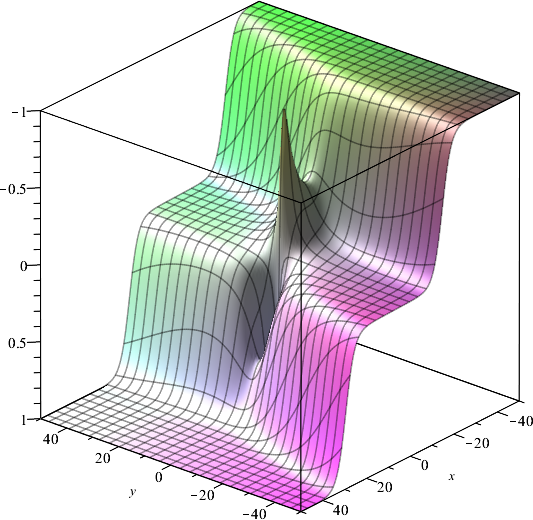
\includegraphics[width=.6\textwidth]{fig/2S1L.png}
\caption{(3+1)JM 方程的 2S-1L 解} \label{fig-2S1L}
\end{figure}

最后, 我们一些方程用 NS1L 求解的结果汇总如\reftab{NS1L-tb}所示. \reftab{NS1L-tb}中统计的运行时间包含了生成方程组\D 求解方程组和过滤等价解这三个步骤的运行时间. 所以这里(3+1)YTSF方程的相关运行时间比上文描述的略长. 此外, (2+1)SK方程和(2+1)BKP-T方程在求 1S-1L 解时分组大小是3, 这是因为分组大小为 5 会无解.

\begin{table}[htbp]
\centering
\caption{NS1L运行结果汇总} \label{NS1L-tb}
\begin{tabular}{cccccc}
\hline
方程名称    & 解的阶数 & 方程数量 & 分组大小 & 解的个数 & 运行时间(s) \\ 
\hline 
(2+1)SK & 0 & 20 & 5 & 1 & 1.875 \\
(2+1)SK & 1 & 65 & 3 & 1 & 3.002 \\
(2+1)SK & 2 & 179 & 5 & 2 & 12.203 \\
(2+1)BKP-T & 0 & 20 & 5 & 1 & 1.110 \\
(2+1)BKP-T & 1 & 65 & 3 & 1 & 3.114 \\
(2+1)BKP-T & 2 & 179 & 5 & 2 & 11.881 \\
(3+1)YTSF & 0 & 35 & 5 & 2 & 1.861 \\
(3+1)YTSF & 1 & 120 & 5 & 3 & 6.928 \\
(3+1)YTSF & 2 & 324 & 5 & 3 & 37.539 \\
(3+1)JM & 0 & 35 & 5 & 4 & 2.702 \\
(3+1)JM & 1 & 120 & 5 & 6 & 14.336 \\
(3+1)JM & 2 & 324 & 5 & 4 & 78.053 \\
\hline 
\end{tabular}
\end{table}
 

\section{小结}
在本章中, 我们提出了一个分组并行的代数方程组求解算法, 并将其实现为 PGSolve 软件包. 作为 PGSolve 的应用实例, 我们编写了用直接代数方法求$n$孤子-1 lump相互作用解的软件包 NS1L. 除了直接对输入方程进行求解之外, PGSolve 还支持自行设定初始解进行求解, 这种方法被称为是继承求解. 在 NS1L 中, 我们可以将低阶的解作为高阶解的初始解进行求解, 能够极大的提升求解的效率. 基于继承求解, 我们能够在10秒内求解含100个左右方程的方程组, 能够在几分钟内求解含300个左右方程的方程组. 

此外, 关于 PGSolve 的使用, 本文总结了以下建议:
\begin{compactenum}[(1)]
\item PGSolve 不能保证或者所有满足要求的解, 它是通过牺牲解的完整性来提升求解效率的.
\item 继承求解能够极大地提升求解效率. 对于一些有包含关系的方程组, 可以先求解小规模的方程组, 再将小规模方程的解作为大规模方程组的初始解进行求解.
\item 在继承求解时, 不一定要将所有的解都作为初始解, 也可以选择一部分形式较为简单的解作为初始解.
\item 调整分组大小将会影响求解的效率和结果. 当单步求解的时间过长时, 应该较小分组大小; 当求解的分支过多时, 应该增加分组大小. 当无解时, 也可以尝试改变分组大小重新求解. 
\end{compactenum}
 

\chapter{n阶展开方法及其应用}\label{ch04}
在微分方程的求解中, 有许多方法都是基于齐次平衡原则发展起来的, 如\Painleve{}展开法\D 双曲正切方法和 Jacobi 椭圆函数方法等. 齐次平衡原则将方程的解设为特定函数的多项式, 通过平衡方程中两个不同最高项的阶数来确定解的阶数. 但是, 在阶数相同的两个最高项平衡时, 齐次平衡原则不能确定阶数的上界, 从而有可能产生漏解的情况. 考虑方程$u(u_t+u_{xxx})+pu_x u_{xx}=0$, 在双曲正切方法和\Painleve{}展开法中, 该方程的阶数列表为$\mbrace{2m+1,2m+3,2m+3}$, 不能基于齐次平衡原则来确定解的阶数. 本文发现, 解的阶数不仅会出现在最高$n$项的阶数中, 还会出现在最高$n$项的系数中. 因此, 本文考虑同时平衡方程中最高$n$项的阶数和系数, 提出了$n$阶展开方法. 

基于$n$阶展开方法能够补充和完善许多基于齐次平衡原则发展起来的方法. 因为非线性差分方程多项式解的求解只涉及多项式的运算, 所以本文将在\refsec{ch4sec1}中以它为例导出$n$阶展开方法. 接着, 我们将在\refsec{ch4sec2}中用图像和例子来形象地解释$n$阶展开方法的原理和作用. 随后, 本文将在\refsec{ch4sec3}中提炼出通用的$n$阶展开方法并实现一个通用的NEM软件包. 基于NEM, 本文在\refsec{ch4sec4}中实现了求非线性差分方程多项式的软件包 NLREPS. 接着, 本文在\refsec{ch4sec5}和\refsec{ch4sec6}中分别以双曲正切方法和\Painleve{}展开法为例阐述$n$阶展开方法在微分方程求解中的应用. 最后, 在\refsec{ch4sec7}中对$n$阶展开方法及其应用进行小结. 

\section{齐次平衡原则与n阶展开方法} \label{ch4sec1}
尽管线性差分方程的求解并没有被完全解决, 但是它的解从多项式解开始变得越来越一般. 受其发展过程的启发, 本文决定求解非线性差分方程的多项式解. 本文求解的方程形如
\begin{equation}
\sum_{k=0}^l{\mbrace{a_k(x)\prod_{i=0}^r{f^{\gamma_{ki}}(x+i)}}}=0,
\label{eq}
\end{equation}
其中 $K$是一个数域, $a_k(x)\in K[x], l>1, \gamma_{ki}\ge 0$. 在本节中, 将基于该方程多项式解的求解导出$n$阶展开方法. 

设
\begin{equation}
f(x)=\sum_{k=0}^m{\mu_kx^k},
\label{fm1}
\end{equation}
将其代入\refeqn{eq}可以求得所有次数不超过$m$的多项式解. 为了求得所有的多项式解, 我们需要找到$m$的上界.

将\refeqn{fm1}代入\refeqn{eq}后, 方程的左端仍然是一个多项式, 这个多项式的各项次数为
\begin{equation}
D = \mbrace{s_1 m+d_1,s_2 m+d_2,\cdots,s_l m+d_l},
\end{equation}
其中
\begin{equation}
\begin{aligned}
s_k&=\sum_{i=0}^r{\gamma_{ki}}, \\
d_k&=\deg a_k(x).
\end{aligned}
\label{eq-sd}
\end{equation}
$D$ 中的每一个次数都是关于 $m$ 的线性表达式, 我们称其为该项的阶数.

方程的左端为零要求整理后的多项式的各项系数为零, 从而要求最高项的系数为零. 因为各个加法项的最高项系数非零, 所以至少有两个不同的最高项进行合并才能使得整理后的多项式最高项系数为零. 从而, 有 
\begin{equation}
\left\{
\begin{array}{l}
m\in \mathbb Z_+  ,                                     \\
\exists i\neq j, s_i m+d_i=s_j m+d_j    ,               \\
\forall k \not\in \bbrace{i,j}, s_i m+d_i\ge s_k m+d_k .
\end{array}
\right.
\label{cond}
\end{equation}
上式中的三个约束条件分别被称为: 整数性约束\D 平衡性约束和最大性约束. 

(I) 如果 $s_i \neq s_j$, 则有 
\begin{equation}
m=\frac{d_j-d_i}{s_i-s_j}.
\end{equation}
如果$m$又同时满足\refeqn{cond}中的其它条件, 则称它为第一类平衡点(简称 \BPone{}). 第一类平衡点构成的集合为 
\begin{equation}
M_1=\bbrace{\left. m=\frac{d_j-d_i}{s_i-s_j}\in \mathbb Z_+\right\vert \forall k\not\in \bbrace{i,j}, s_i m+d_i\ge s_k m+d_k}.
\end{equation}

(II) 如果 $s_i = s_j, d_i=d_j$, 则能始终满足平衡性约束. 考虑最大性约束, 则有 
\begin{equation}
\left\{
\begin{aligned}
m > \frac{d_k-d_i}{s_i-s_k}, & \text{ if } s_i>s_k,  \\
m < \frac{d_k-d_i}{s_i-s_k}, & \text{ if } s_i<s_k.  \\
\end{aligned}
\right.
\end{equation}
因为\BPone{}的成立条件已经包含上述不等式中取等号的条件, 所以上述不等式不含等号. 求解上述不等式, 可以得到 
\begin{equation}
\underset{s_i>s_k}{\max}{\frac{d_k-d_i}{s_i-s_k}} < m < \underset{s_i<s_k}{\min}{\frac{d_k-d_i}{s_i-s_k}}.
\end{equation}
如果 $s_i m + d_i < \sigma m + \delta$, 则$m$存在上界. 这里, 
\begin{equation}
\begin{aligned}
\sigma &= \max ~s_k,  \\
\delta &= \underset{s_k=\sigma}{\max}{~d_k}.
\end{aligned}
\label{eq-max-sd}
\end{equation}

我们将根据$m$是否存在上界, 分两种情况进一步讨论:

(II-a) 当 $s_i m + d_i < \sigma m + \delta$时, $m$的取值范围有限. 可以得到第二类平衡点(简称 \BPtwo{}). 第二类平衡点构成的集合为
\begin{equation}
M_2=\bbrace{m\in \mathbb Z_+\left|\underset{s_i>s_k}{\max}{\frac{d_k-d_i}{s_i-s_k}} < m < \underset{s_i<s_k}{\min}{\frac{d_k-d_i}{s_i-s_k}}\right.} .
\end{equation}

(II-b) 当 $s_i m + d_i = \sigma m + \delta$ 时, 无法基于齐次平衡原则来确定$m$的上界. 因此, 我们提出了一个$n$阶展开方法来解决这个问题.

给定 $n>0$, 定义一个$m$次多项式的$n$阶展开形式为
\begin{equation}
F\sbrace{x,m,u\up n}=\sum_{k=0}^{n-1}{u_k x^{m-k}}+\OO\sbrace{x^{m-n}},
\label{npoly}
\end{equation}
其中 $u\up n=\mbrace{u_0,u_1,\cdots,u_{n-1}}$是系数向量, 而
\begin{equation}
\OO\sbrace{x^n}=\left\{
\begin{array}{cl}
\text{次数不超过}\,n\,\text{的多项式} & n\ge 0, \\
0                                    & n<0 .
\end{array}
\right.
\end{equation}

对于未知的$m$次多项式$f(x)$, 设其最高$n$项的系数为$u\up n=\mbrace{u_0,u_1,\cdots,u_{n-1}}$, 则它可以表示为 
\begin{equation}
f(x)=F\sbrace{x,m,u\up n}. \label{nepoly-f}
\end{equation}

对于一个具体的多项式
\begin{equation}
a_k(x)=\sum_{i=0}^{d_k}{a_{k,i} x^{d_k-i}}, \label{nepoly-a}
\end{equation}
设
\begin{equation}
\alpha_{k,i}=\left\{
\begin{array}{cl}
a_{k,i} & i\le \min\{n-1,d_k\}, \\
0       & i >  \min\{n-1,d_k\},
\end{array}
\right.
\end{equation}
则有
\begin{equation}
a_k(x)=F\sbrace{x,d_k,\alpha_k\up n},
\end{equation}
其中 $\alpha_k\up n=\mbrace{\alpha_{k,0},\alpha_{k,1},\cdots,\alpha_{k,n-1}}$.

于是, 在确定$n$阶展开多项式的基本运算规则之后, 就能将\refeqnn{eq}的左端改写为一个$n$阶展开多项式.

首先, 考虑移位操作
\begin{equation}
\Delta^r F\sbrace{x,m,u\up n} = F\sbrace{x+r,m,u\up n} = f(x+r).
\end{equation}
当 $r\neq 0$ 时, 有 
\begin{equation} 
\begin{aligned}
\Delta^r F\sbrace{x,m,u\up n} &= \sum_{k=0}^{n-1}{u_k (x+r)^{m-k}}+\OO\sbrace{x^{m-n}} \\
&= \sum_{k=0}^{n-1}{u_k \mbrace{\sum_{j=0}^{m-k}{\binom{m-k}{j}r^j x^{m-k-j}}}}+\OO\sbrace{x^{m-n}} \\
&= \sum_{k=0}^{n-1}{u_k \mbrace{\sum_{m-k-j>m-n}{\binom{m-k}{j}r^j x^{m-k-j}}}}+\OO\sbrace{x^{m-n}} \\
&= \sum_{k+j<n}{u_k {\binom{m-k}{j}r^j x^{m-k-j}}}+\OO\sbrace{x^{m-n}} \\
&=\sum_{p=0}^{n-1}{x^{m-p}\mbrace{\sum_{k=0}^p{u_k\binom{m-k}{p-k}r^{p-k}}}}+\OO\sbrace{x^{m-n}}\\
&=F\sbrace{x,m,v\up n}.
\end{aligned} \label{NEM-shift}
\end{equation}
其中 $v\up n=\mbrace{v_0,v_1,\cdots,v_{n-1}}$, 而
\begin{equation}
v_p=\sum_{k=0}^p{u_k\binom{m-k}{p-k}r^{p-k}}.
\end{equation}

注意到系数$v_p$是关于$m$的多项式, 所以我们不仅可以基于次数来分析$m$的取值, 还能基于系数来分析$m$的取值. 

然后, 考虑乘法 
\begin{equation}
\begin{aligned}
& F\sbrace{x,m,u \up n}\cdot F\sbrace{x,l,v\up n} \\
=& \mbrace{\sum_{k=0}^{n-1}{u_k x^{m-k}}+\OO\sbrace{x^{m-n}}}\mbrace{\sum_{k=0}^{n-1}{v_k x^{l-k}}+\OO\sbrace{x^{l-n}}} \\
=& \mbrace{\sum_{k=0}^{n-1}{u_k x^{m-k}}}\mbrace{\sum_{k=0}^{n-1}{v_k x^{l-k}}}+\OO\sbrace{x^{m+l-n}} \\
=& \sum_{p=0}^{n-1}{x^{m+l-p}\mbrace{\sum_{k=0}^p{u_k v_{p-k}}}}+\OO\sbrace{x^{m+l-n}} \\
=& F\sbrace{x,m+l,w\up n} ,
\end{aligned} \label{NEM-times}
\end{equation}
其中 $w\up n=\mbrace{w_0,w_1,\cdots,w_{n-1}}$, 而
\begin{equation}
w_p=\sum_{k=0}^p{u_k v_{p-k}}.
\end{equation}

在确定了乘法和移位操作之后, 就能将\refeqnn{eq}中的每个加法项重写为$n$阶展开多项式, 即
\begin{equation}
\begin{aligned}
a_k(x)\prod_{i=0}^r{f^{\alpha_{ki}}(x+r)}&=F\sbrace{x,d_k,\alpha_k\up n}\prod_{i=0}^r{\Delta^{\gamma_{ki}}F\sbrace{x,m,u\up n}} \\
&= F\sbrace{x,s_k m+d_k, \omega_k\up n} .
\end{aligned}
\end{equation}

最后, 考虑更为复杂的加法: 
\begin{equation}
F\sbrace{x,s_i m+d_i,u\up n}+F\sbrace{x,s_j m+d_j,v\up n}.
\end{equation}
一般情况下, 我们不能在$m$未知的情况下比较 $s_i m + d_i$ 和 $s_j m + d_j$ 大小. 但是, 假设
\begin{equation}
s_i m+d_i-n > s_j m+d_j, \label{cond_add}
\end{equation}
可以有 
\begin{equation}
\begin{aligned}
&F\sbrace{x,s_i m+d_i,u\up n}+F\sbrace{x,s_j m+d_j,v\up n} \\
=&\left\{
\begin{array}{cl}
    F\sbrace{x,s_i m+d_i,u\up n} & s_i>s_j,            \\
    F\sbrace{x,s_i m+d_i,w\up n} & s_i=s_j,
\end{array}
\right.
\end{aligned} \label{NEM-add}
\end{equation}
其中
\begin{equation}
w_p=\left\{
\begin{array}{cl}
u_p               & p<d_i-d_j ,   \\
u_p+v_{p-d_i+d_j} & p\ge d_i-d_j.
\end{array}
\right.
\end{equation}

最终, \refeqnn{eq} 能够被重写为
\begin{equation}
F(x,\sigma m + \delta,\Omega\up n)=0, 
\label{eq-np}
\end{equation}
其中 $\Omega\up n=\mbrace{\Omega_0,\cdots,\Omega_{n-1}}$, 而 $\Omega_k$ 则是关于 $m$ 和 $u_k$ 的多项式.

在情况(II-b)的条件下, 由\refeqn{cond_add}可知, 若要使\refeqn{eq-np}中的第$k~(k=0,1,\cdots)$个系数有效, 则需满足 
\begin{equation}
\forall s_j<\sigma, \sigma m + \delta - k > s_j m + d_j,
\end{equation}
即
\begin{equation}
m > \underline{m}_k=\underset{s_j<\sigma}{\max}{\frac{d_j-\delta+k}{\sigma-s_j}}.
\end{equation}

现在我们可以来寻找第三类平衡点(简称\BPthree{}). 因为\refeqnn{eq}的左端非零, 因此当$n$足够大时, 必然存在一个$\Omega_k\neq 0$. 设$\Omega_{k_0}$是第一个非零项. 

如果 $\Omega_{k_0}=0$ 关于 $m$ 有非负整数解 $m_0$, 则解的次数必然不超过 $m_0$. 同时, $\Omega_{k_0}$ 的有效性又要求 $m>\underline{m}_{k_0}$. 所以, 此类\BPthree{}所构成的集合为 
\begin{equation}
M_3=\bbrace{m\in \mathbb Z_+|\max\sbrace{M_1\cup M_2 \cup \bbrace{\underline{m}_{k_0}}}<m\le m_0}. \label{BP31}
\end{equation}

如果 $\Omega_{k_0}=0$ 关于 $m$ 没有非负整数解, 就意味着当 $\Omega_{k_0}$有效时(即$m>\underline{m}_{k_0}$时), 方程没有多项式解. 因此, 方程有多项式解的必要条件是 $m\le \underline{m}_{k_0}$. 从而, 此类\BPthree{}构成的集合为 
\begin{equation}
M_3=\bbrace{m\in \mathbb Z_+|\max\sbrace{M_1\cup M_2}<m\le \underline{m}_{k_0}}. \label{BP32}
\end{equation}

最终, 可以确定$m$的上界, 即
\begin{equation}
\overline m =\max\sbrace{M_1\cup M_2\cup M_3}.
\end{equation}
将 $f(x)=\sum_{k=0}^{\overline m}{\mu_k x^k}$ 代入 \refeqnn{eq}, 我们就能求得所有的多项式解.

\section{方法的可视化与典型例子}\label{ch4sec2}
基于\refeqn{cond}中的三个约束条件, 我们确定了解的次数的上界. 因为方程中每一项的次数都是关于$m$的线性表达式, 所以它们能够被看成是平面上的一条直线. 设各项次数为 
\begin{equation}
\lambda_1(m),\cdots,\lambda_l(m), \label{lines}
\end{equation}
其中 $\lambda_k(m)=s_k m+d_k$. 我们的算法等价于在折线
\begin{equation}
\lambda(m)=\max\bbrace{\lambda_1(m),\cdots,\lambda_l(m)} \label{broken_line}
\end{equation}
上寻找两条不同直线的整数交点. 

例如在\reffig{point}中, 有7条直线, 它们分别被记为$\lambda_1,\cdots,\lambda_7$. 我们用虚线表示\refeqn{lines}中的直线, 用实线表示\refeqn{broken_line}中的折线. 这些直线的交点被标记为$B_1,\cdots,B_8$, 并且我们假设它们都是整点. 
\begin{figure}[htbp]
\centering
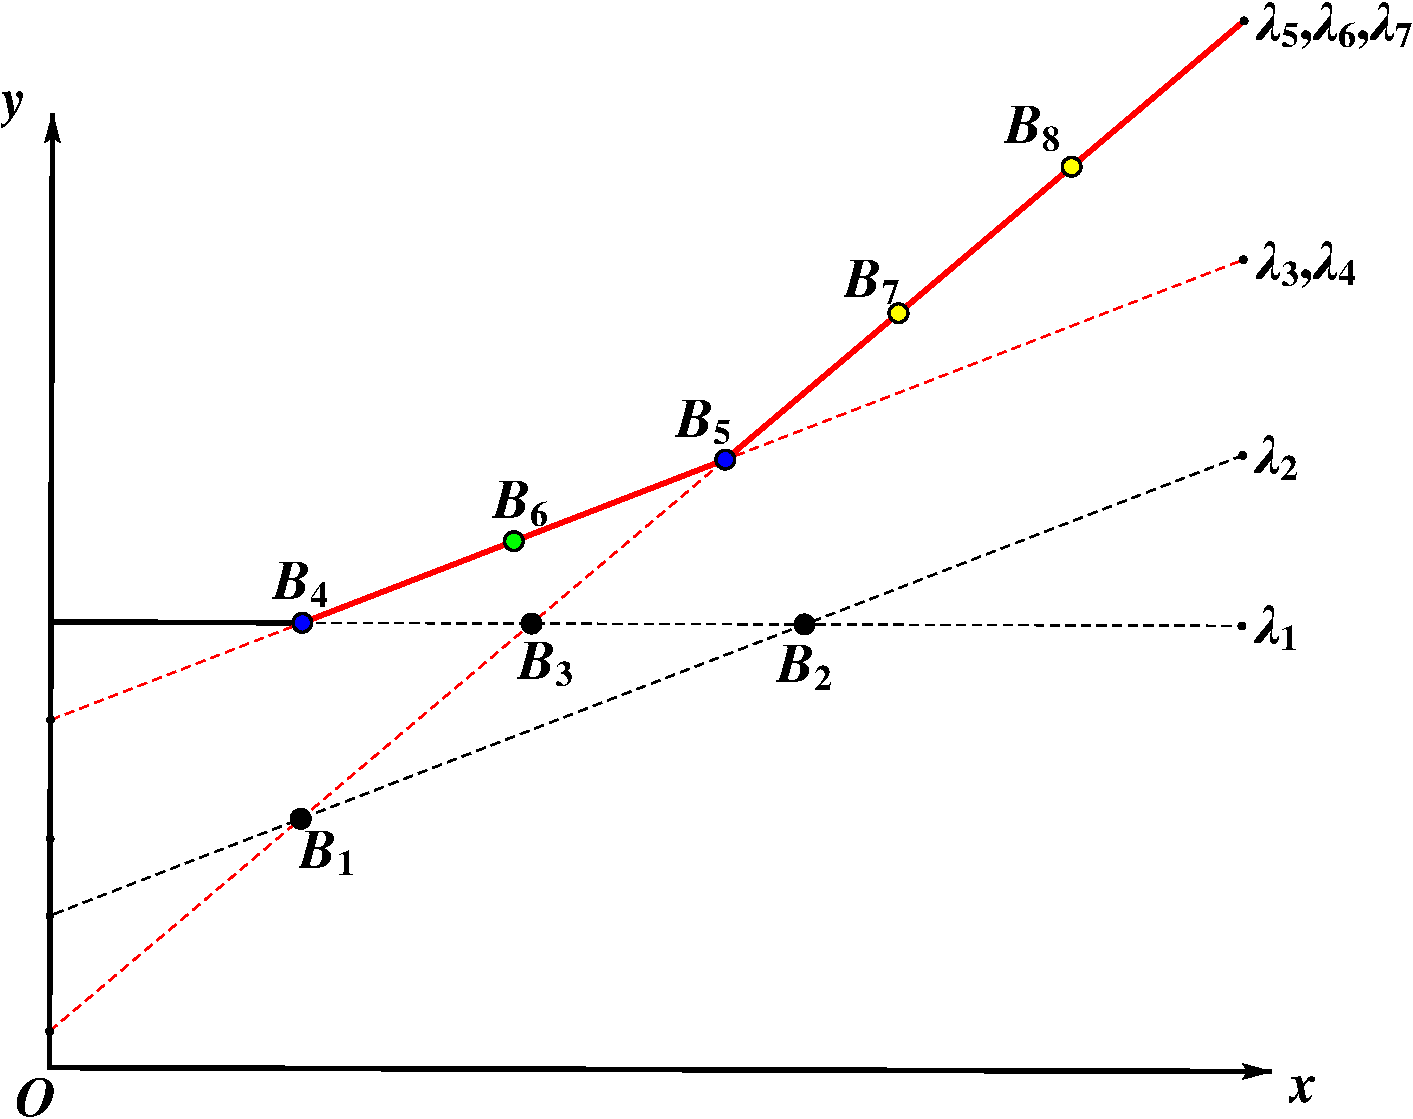
\includegraphics[width=0.6\textwidth]{fig/ps.pdf}
\caption{$n$阶展开方法的平衡点分类示意图}
\label{point}
\end{figure}
\begin{compactitem}[\textbullet]
\item 尽管$B_1,B_2,B_3$是不同直线的交点, 但是因为它们不满足最大性约束, 所以他们不是平衡点. 
\item 而$B_4,B_5$ 是不同直线的交点且满足最大性约束, 所以它们是第一类平衡点.
\item $B_6$虽然不是不同直线的交点, 但有多条直线穿过它. 又因为它在$B_4$ 和 $B_5$ 之间, 所以它是第二类平衡点.
\item 因为有多条重复直线穿过$B_7,B_8$以及它们右侧更多的整点, 且它们的右侧没有其它直线的交点, 所以它们是可能的第三类平衡点. 我们可以通过$n$阶展开方法来确定这一类平衡点的上界.
\end{compactitem}

下面将给出一些具有代表性的例子. 

\begin{example}
(\BPone{})
\begin{equation}
-x^4f(x+3)+(x+1)f(x)^2+8x^6+27x^5+28x^4+2x^3-x-1=0 \label{ep1} .
\end{equation}

该方程的阶数列表为$[m+4,2m+1,6]$. 因为没有重复的次数, 所以该方程只有\BPone{}. 基于 $m+4=6,2m+1=6$ 和 $m+4=2m+1$ 可以得出 $M_1=\{2,3\}$, 从而$\overline m = 3$. 然后, 将$f(x)=\sum\nolimits_{k=0}^3{\mu_k x^k}$ 代入原方程, 可得到如下方程组:
\begin{equation}
\left\{
\begin{array}{l}
    {\mu_{{0}}}^{2}-1=0,                                                                                                  \\
    {\mu_{{3}}}^{2}-\mu_{{3}}=0,                                                                                            \\
    {\mu_{{0}}}^{2}+2\,\mu_{{0}}\mu_{{1}}-1=0,                                                                                \\
    2\,\mu_{{0}}\mu_{{1}}+2\,\mu_{{0}}\mu_{{2}}+{\mu_{{1}}}^{2}=0,                                                                \\
    2\,\mu_{{2}}\mu_{{3}}+{\mu_{{3}}}^{2}-\mu_{{2}}-9\,\mu_{{3}}+8=0,                                                             \\
    2\,\mu_{{0}}\mu_{{2}}+2\,\mu_{{0}}\mu_{{3}}+{\mu_{{1}}}^{2}+2\,\mu_{{1}}\mu_{{2}}+2=0,                                            \\
    2\,\mu_{{1}}\mu_{{3}}+{\mu_{{2}}}^{2}+2\,\mu_{{2}}\mu_{{3}}-\mu_{{1}}-6\,\mu_{{2}}-27\,\mu_{{3}}+27=0,                              \\
    2\,\mu_{{0}}\mu_{{3}}+2\,\mu_{{1}}\mu_{{2}}+2\,\mu_{{1}}\mu_{{3}}+{\mu_{{2}}}^{2}-\mu_{{0}}-3\,\mu_{{1}}-9\,\mu_{{2}}-27\,\mu_{{3}}+28=0.
\end{array}
\right.
\label{ceqs}
\end{equation}
可以求出\refeqnn{ceqs}的解为$\{\mu_0=-1,\mu_1=0,\mu_2=0,\mu_3=1\}$. 最终, \refeqnn{ep1}的多项式解为$f(x)=x^3-1$.
\end{example}

\begin{example}
(\BPtwo{})
\begin{equation}
x^2f(x)f(x+1)f(x+2)+(1-x^9)f(x)+(x^4-x^9)f(x+1)+2x^9f(x+2)-\sum_{k=0}^{10}{c_k x^k}=0, \label{ep2}
\end{equation}
其中$[c_0,\cdots,c_{10}]=[1,1,22,57,85,72,35,9,1,10,6]$. 该方程的阶数列表为$[3m+2,m+9,m+9,m+9,10]$. 从$m+9=10$可以得到第一类平衡点$M_1=\{1\}$. 因为$m+9$有多个, 且它关于$m$的系数不是最大的, 所以该方程有\BPtwo{}. 从$\{m+9> 10,m+9> 3m+2\}$可以得出$m< 7/2$. 因此, $\overline m=3$. 然后, 可以解得原方程的多项式解为$f(x)=x^2+x+1$. 显然, 如果不考虑\BPtwo{}, 我们将无法求出该方程的多项式解. 
\end{example}

\begin{example} \label{examp-3}
(\BPthree{}, 2阶展开)
\begin{equation}
(x+2)f(x)-(x-1)f(x+1)=0. \label{ep3}
\end{equation}
因为该方程的阶数列表为$[m+1,m+1]$, 所以它只有\BPthree{}. 基于2阶展开, 即将$f(x)=u_0 x^m + u_1 x^{m-1} + \OO(x^{m-2})$ 代入到原方程中, 可以得到
\begin{equation}
(-u_0 m+3u_0)x^m+\OO(x^{m-1})=0.
\end{equation}
从 $-u_0 m+3u_0=0$ 可以解得 $m=3$. 然后, 可以解得该方程的多项式解 $f(x)=c(x^3-x)$, 其中 $c$ 是任意常数. 
\end{example}

\begin{example}
(\BPthree{}, 高阶展开)
\begin{equation}
-2x^5f(x)f(x+2)+x^4f(x)^2+(2x^5-x^4)f(x+1)^2-\sum_{k=0}^{22}{c_k x^k}=0, \label{ep4}
\end{equation}
其中 $[c_0,\cdots,c_{22}]=$[0, 0, 0, 0, 1, 2046, 10140, 22340, 28095, 20730, 7788, 6120, 30600, 84180, 151164, 199504, 199710, 151380, 85560, 35136, 10035, 1830, 170]. 该方程的阶数列表为 $[2m+5,2m+4,2m+5,22]$. 由 $2m+5=22$ 可得 $ m=17/2$, 该方程没有\BPone{}. 所以该方程只有\BPthree{}. 在该方程的$n$阶展开中, 第一个非零项为 
\begin{equation}
\Omega_3 = 2m^2u_0^2-3mu_0^2-2u_0u_1.
\end{equation}
因为$\Omega_3=0$关于$m$没有正整数解, 所以当$\Omega_3$有效时, 方程没有多项式解. 换句话说, 只有$2m+5>22+3$不成立, 即$m\le 10$时, 才有多项式解. 从而, $\overline m =10$, 可以得到\refeqnn{ep4} 的多项式解为 $f(x)=\pm (x^{10}-1)$.
\end{example}

\begin{example}
(应用, 2阶展开)

为了计算 
\begin{equation}
    S(x)=\sum_{k=0}^x{k^{10}}
\end{equation}
的闭形式解, 可以构造差分方程
\begin{equation}
    S(x)-S(x-1)=x^{10}, S(0)=0. \label{seq}
\end{equation}
该方程的阶数列表为$\mbrace{m,m,10}$. 此时, $m=10$ 是 \BPone{}. 因为这里有两个重复的$m$, 所以需要考虑\BPthree{}. 该方程的 2 阶展开为
\begin{equation}
u_0m x^{m-1}+\OO(x^{m-2})=0.   
\end{equation}
因为当$m-1>10$时, $\Omega_1=u_0m$有效, 方程没有多项式解. 所以, 必须有$m\le 11$. 从而, $\overline m=11$, 可以得到原方程的多项式解为
\begin{equation}
S(x)=\frac{5}{66}x-\frac{1}{2}x^3+x^5-x^7+\frac{5}{6}x^9+\frac{1}{2}x^{10}+\frac{1}{11}x^{11}.
\end{equation}
对这个例子, 如果不考虑第三类平衡点, 我们将不能获得其多项式解. 

另一方面, \refeqnn{seq}是一个线性方程, 也可以采用其它方法\cite{Abramov1989polynomial,Abramov1995polynomial}求其多项式解. 但是, 这个方程在我们的方法中是通过2阶展开求解的, 这也说明了$n$阶展开的必要性. 
\end{example}

\begin{example}
(应用, logistic方程, 也称虫口方程)

因为我们的算法可以求出所有的多项式解, 所以如果基于我们的算法没有获得多项式解则表示方程没有多项式解. 考虑著名的logistic 方程\cite{may1976simple}
\begin{equation}
    f(x+1)=r f(x)\sbrace{1-f(x)},
\end{equation}
其中 $r$ 是一个常数. 该方程的阶数列表为 $\mbrace{2m,m,m}$. 因为 $2m\ge m$, 所以该方程只有\BPone{}, 即$2m=m\Rightarrow m=0$. 可以的得出, 该方程除了$f(x)=0$和$f(x)=(r-1)/r$以外, 没有其它非平凡的多项式解.
\end{example}

\begin{example}
(应用, Riccati方程)

对于 Riccati 方程\cite{bittanti2012riccati}
\begin{equation}
    f(x+1)f(x)+A(x)f(x)+B(x)f(x+1)=C(x), \label{raeq}
\end{equation} 
其中$A(x),B(x)$ 和 $C(x)$ 是多项式系数, 我们取 
\begin{equation}
\begin{aligned}
A(x)&= -\frac{1}{2}\sbrace{x^5+5x^4-40x^2-2}, \\ 
B(x)&= -\frac{1}{2}\sbrace{x^5+10x^3-x-2}, \\ 
C(x)&= -x\sbrace{x+1}\sbrace{48x^4+20x^2-5x-3}.
\end{aligned}
\end{equation}
该方程的阶数列表为$\mbrace{2m,m+5,m+5,6}$. 对于该方程的平衡点的分类讨论如\reftab{tb}所示.

\begin{table}[htbp]
\centering
\caption{关于 Riccati 方程的平衡点的分类讨论}\label{tb}
\begin{tabular}{ccc}
\hline
平衡点类型 & 平衡方程 & 平衡点  \\ 
\hline
\BPone{}  & $2m=m+5\ge 6$            & $m=5$             \\ 
\BPone{}  & $2m=6\ge m+5$            & $m\in \varnothing$             \\ 
\BPone{}  & $m+5=6\ge 2m$            & $m=1$             \\ 
\BPtwo{}  & $m+5>\max\bbrace{2m,6}$  & $m\in \bbrace{2,3,4}$ \\
\hline
\end{tabular}
\end{table}
从\reftab{tb}中可以得出: $M_1=\bbrace{1,5},M_2=\bbrace{2,3,4}$. 因此, $\overline m=5$. 最终, 可以得到该方程的多项式解 $f(x)=x^5-x$. 

在 Maple 中, 使用 \cd{rsolve} 求解\refeqnn{raeq}会得到
\begin{equation}
\begin{aligned}
    f(x)&=(f \left( 0 \right) \alpha(x)\,{x}^{5}+f \left( 0 \right) \beta(x)\,{x}^{5}+10\,f \left( 0 \right) \alpha(x)\,{x}^{3}\\
    &-10\,f \left( 0 \right) \beta(x)\,{x}^{3}+2\,{x}^{5}-f \left( 0 \right) \alpha(x)\,x-f \left( 0 \right) \beta(x)\,x\\
    &-2\,f \left( 0 \right) \alpha(x)+2\,f \left( 0 \right) \beta(x)-2\,x)/(2+2f(0)\alpha(x)) ,
\end{aligned} \label{rasol_real}
\end{equation}
其中
\begin{equation}
\begin{aligned}
&\alpha(x)=\sum_{k_1=0}^{x-1}\mbrace{
    \frac{(-1)^{k_1}p(k_1)}{q(k_1)}\prod_{k_0=0}^{k_1}{
        \frac{q(k_0)}{p(k_0)}
    }
}, \\
&\beta(x)=\sum_{k_1=0}^{x}\mbrace{
    \frac{(-1)^{k_1}p(k_1)}{q(k_1)}\prod_{k_0=0}^{k_1}{
        \frac{q(k_0)}{p(k_0)}
    }
}, \\
&p(x)=x^5+5x^4-20x^2-26x+8, \\
&q(x)=x^5+5x^4+20x^3+10x^2+8x+2. 
\end{aligned}
\end{equation}
将 $f(0)=0$ 代入\refeqn{rasol_real}, 可以得到 $f(x)=x^5-x$. 这表示该多项式解是在初始条件 $f(0)=0$ 下的解. 此外, 需要注意的是, 使用 \cd{LRETools[riccati]} 来求解\refeqnn{raeq}将得到错误的解, 这显然是该函数的一个BUG. 
\end{example}

\section{NEM软件包的实现}\label{ch4sec3}
在上文中, 我们以差分方程多项式解的求解为例, 阐述了$n$阶展开方法的思路和步骤. 实际上, $n$阶展开方法也能用于完善其它基于齐次平衡原则发展起来的方法. 为了能够更方便地将$n$阶展开方法应用到相关问题中, 本文决定将$n$阶展开方法单独实现为 NEM 软件包.

从上文的分析可以看出, 在计算\BPone{}和\BPtwo{}时, 只需要关注方程的各项次数, 而计算\BPthree{}则需要借助于$n$阶展开多项式来计算最高$n$的系数. 事实上, 只要列出了$n$阶展开多项式, 也能获得方程各项的次数. 因此, 我们将$n$阶展开多项式作为NEM的输入对象. 在应用到具体问题时, 只需将对应问题中的各项转化为$n$阶展开多项式, 就能调用NEM来确定平衡点的上界, 后续的求解则交给对应问题的相关程序进行解决. 

在NEM软件包中, 我们将$n$阶展开多项式实现为\cd{NEPoly}对象. \cd{NEPoly}对象有三个关键属性: $p,q$和$u$. 其中 $pm+q$就是该多项式的次数, 而$u$则是最高$n$项的系数. 并且, \cd{NEPoly}对象还根据\refeqn{NEM-shift}\D \refeqn{NEM-times} 和 \refeqn{NEM-add} 分别实现了移位\D 乘法和加法操作. 此外, 为了能够将程序应用到微分方程求解的相关问题中, 我们还推导了微分的计算规则:
\begin{equation}
\begin{aligned}
& \DIF{t}F\sbrace{x,m,u\up{n}}  \\
=& \DIF{t}\sbrace{\sum_{k=0}^{n-1}{u_k x^{m-k}}+\OO(x^{m-n})} \\
=& \sum_{k=0}^{n-1}{\DIFF{u_k}{t}x^{m-k}}+\DIFF{x}{t}\cdot\sum_{k=0}^{n-1}{u_k (m-k) x^{m-k-1}}+\DIFF{x}{t}\cdot\OO(x^{m-n-1}) \\
=& \sum_{k=0}^{n-1}{\DIFF{u_k}{t}x^{m-k}}+\DIFF{x}{t}\cdot\sbrace{\sum_{k=0}^{n-1}{u_k (m-k) x^{(m-1)-k}}+\OO\sbrace{x^{(m-1)-n)}}} \\ 
=& F\sbrace{x,m,v\up{n}}+\DIFF{x}{t}\cdot F\sbrace{x,m-1,w\up{n}}, 
\end{aligned}\label{NEM-diff}
\end{equation}
其中 
\begin{equation}
v_p=\DIFF{u_p}{t}, w_p=u_p(m-p).
\end{equation}
只需将$\DIFF{x}{t}$也表示成关于$x$的$n$阶展开多项式, 就能使得\cd{NEPoly}关于导数的计算结果也是$n$阶展开多项式. 

在实现了\cd{NEPoly}之后, 我们实现了NEM的核心接口\cd{nem(vs)}, 其输入参数\cd{vs}是一个\cd{NEPoly}列表, 表示方程中各个加法项转化为$n$阶展开多项式的结果. \cd{nem(vs)}的核心逻辑如\refalg{nem}所示. 

\begin{algorithm}[H]
\newcommand{\kw}[1]{\mathbf{~#1~}}
\newcommand{\Fcn}[1]{\mathtt{#1}}
\renewcommand{\lfrac}[2]{\sbrace{#1}/\sbrace{#2}}
\caption{$n$阶展开方法的核心算法 \cd{nem(vs)}}\label{nem}
\KwIn{\cd{NEPoly}对象的列表.}
\KwOut{平衡点上界, $-\infty$ 表示没有找到平衡点.}
$s,d,\sigma,\delta,l\gets \Fcn{getOrders}(vs)$\tcp*[r]{从输入对象中获取相关次数}
$m_1,m_2,m_3\gets -\infty$\tcp*[r]{初始化三种类型平衡点的上界.}
$needBP3\gets\kw{false}$\tcp*[r]{用于记录是否需要 \BPthree{}.}
\For{$i \kw{from} 1 \kw{to} l$}{\label{for-1-start}
    \For{$j \kw{from} i+1 \kw{to} l$}{
        \uIf(\tcp*[f]{寻找 \BPone{}.}){$s_i\neq s_j$}{
            $m\gets (d_j-d_i)/(s_i-s_j)$\;
            \If{$m\in \mathbb Z_+ \kw{and} s_im+d_i\ge \max\{s_km+d_k\}$}{
                $m_1\gets \max(m,m_1)$\;
            }
        }\ElseIf(\tcp*[f]{寻找 \BPtwo{}.}){$s_i=s_j \kw{and} d_i=d_j$}{
            \If(\tcp*[f]{判定是否需要\BPthree{}.}){$s_i=\sigma \kw{and} d_i=\delta$}{
                $needBP3\gets \kw{true}$;~\textbf{continue}\;
            }
            $lb\gets \floor{\underset{s_i>s_k}{\max}{\lfrac{d_k-d_i}{s_i-s_k}}}+1$\;
            $ub\gets \ceil{\underset{s_i<s_k}{\min}{\lfrac{d_k-d_i}{s_i-s_k}}}-1$\;
            \If{$ub\neq +\infty \kw{and} lb\le ub \kw{and} ub\ge 0$}{
                $m_2\gets \max(ub,m_2)$\;
            }
        }
    }
}\label{for-1-end}
\If(\tcp*[f]{寻找 \BPthree{}.}){$needBP3$}{
    $r\gets \sum_{v\in vs}{v}$;~$\Omega\gets r.u$\; \label{add-nem}
    \For{$k \kw{from} 0 \kw{to} n-1$}{\label{for-2-start}
        \If{$\Omega_k\neq 0$}{
            $sol\gets \Fcn{solve}(\Omega_k=0,m)$\;
            $m_{31}\gets \max(sol \bigcap \mathbb{Z}_+)$\tcp*[r]{有解时的上界}
            $m_{32}\gets \floor{\underset{s_j<\sigma}{\max}{\lfrac{d_j-\delta+k}{\sigma-s_j}}}$\tcp*[r]{无解时的上界}
            $m_3\gets \max(m_{31},m_{32})$\;
            \textbf{break}\;
        }
    }\label{for-2-end}
    \If{$m_3=-\infty$}{
        \cd{warning}(`$n$ need be increased.')\;
    }
}
\Return{$\overline m= \max(m_1,m_2,m_3)$}\;
\end{algorithm}

在\refalg{nem}中, 首先按照前文的定义, 从\cd{NEPoly}对象中提取相关次数. 然后, 在\refcln{for-1-start}到\refcln{for-1-end}中, 基于这些次数寻找\BPone{}和\BPtwo{}. 在此过程中, 我们也会检测当前问题是否需要继续寻找\BPthree{}. 在这个过程中, 需要对$l$个输入项进行两两比较, 在内部的计算中也需要寻找这$l$个对象中的相关最值, 所以, 这个过程的时间复杂度为$\OC(l^3)$.

若需要继续计算\BPthree{}, 我们将在\refcln{add-nem}中对输入的\cd{NEPoly}对象求和, 然后在\ref{for-2-start}-\ref{for-2-end}行中寻找\BPthree{}. 这里, $m_{31}$是$\Omega_{k_0}=0$关于$m$有解时\BPthree{}的上界, 而$m_{32}$则是无解时的上界. 因为这两者在其中一个非负时, 另一个必然为$-\infty$, 所以可以取两者的最大值来确定\BPthree{}的上界. 事实上, $m_{31}$和$m_{32}$分别对应了\refeqn{BP31}和\refeqn{BP32}的上界. 此外, 如果在当前$n$项中并未找到非零系数, 则程序会提醒用户增大展开阶数继续尝试. 在这一部分, 程序首先对$l$个输入项求和, 这部分时间复杂度为$\OC(nl)$. 然后, 程序要在$n$个展开系数中寻找非零项, 找到之后需要计算$l$个输入项的最值, 不考虑求解方程的复杂度, 则其时间复杂度为$\OC(n+l)$.

最后, 取三类平衡点的最大值就能确定平衡点的上界. 最终, \refalg{nem}的时间复杂度为$\OC(l^3+nl+n+l)$. 当$n$没有远大于$l$时, \refalg{nem}的时间复杂度等价于$\OC(l^3)$.

\section{NLREPS 软件包的实现与测试}\label{ch4sec4}

基于NEM, 我们实现了求解非线性差分方程多项式解的软件包NLREPS.
\begin{compactenum}[(1)]
\item 首先, 对于形如\refeqn{eq}的输入方程, 将各项系数$a_k(x)$用\refeqn{nepoly-a}转化为\cd{NEPoly}对象, 将未知函数$f(x)$按照\refeqn{nepoly-f}转化为\cd{NEPoly}对象. 
\item 然后, 调用\cd{NEPoly}的内置功能, 基于\refeqn{NEM-shift}计算移位, 基于\refeqn{NEM-times}计算乘法, 得到各个加法项对应的\cd{NEPoly}对象. 
\item 接着, 通过调用\refalg{nem}中的\cd{nem}函数, 计算平衡点的上界$\overline{m}$.
\item 最后, 用待定系数法, 将$f(x)=\sum_{k=0}^{\overline{m}}{\mu_k x^k}$代入原方程求解即可. 
\end{compactenum}

按照上述方法, 我们实现了NLREPS, 其核心接口为
\begin{verbatim}
nlreps(eq,fx,{nExpand,inits});
\end{verbatim}
其中
\begin{compactitem}[\textbullet]
\item \cd{eq} 表示输入的方程.
\item \cd{fx} 表示需要求解的未知函数, 如$f(x)$.
\item \cd{nExpand} 表示展开阶数. 这个参数是可选的, 默认值为\cd{nExpand=5}. 
\item \cd{inits} 表示初始条件, 例如 \cd{\{f(0)=0, f(1)=1\}}. 这个参数也是可选的, 默认为空集, 表示没有初始条件. 
\end{compactitem}

例如, 对于例\ref{examp-3}中的问题, 若添加初始条件$\{f(0)=-1\}$, 并指定展开阶数为4, 则调用方式为
\begin{verbatim}
nlreps(eq,f(x),nExpand=4,inits={f(0)=-1});
\end{verbatim}
然后, 就能得到解 $\{f(x)=x^{10}-1\}$.

为了测试NLREPS的求解性能, 我们随机生成了1000个不同规模的问题进行测试. 我们产生测试用例的方法如下: 将 
\begin{equation}
    F=\sum_{k=0}^l{\mbrace{a_k(x)\prod_{i=0}^r{f^{\gamma_{ki}}(x+i)}}}
\end{equation}
看作是关于$f(x),\cdots,f(x+r)$的多元多项式, 其系数为 $a_k(x)$. 对于这个多项式, 取
\begin{equation}
\begin{aligned}
&\max{\rm deg}(a_k(x))=\max d_k=10,\\ 
&\max{\rm deg}(F)=\max s_k=5, \\
&l\in [2,400], r=5.
\end{aligned}
\end{equation}
生成$F$之后, 我们生成一个随机的解$f^*(x)$代入$F$得到$g(x)$, 最终得到方程$F-g(x)=0$. 其中 ${\rm deg}(f^*(x))\le 10$. 生成1000个测试用例之后, 我们从3个方面对它们进行分析. 

首先, 我们考虑测试\cd{nlreps}的运行时间. 因为求解代数方程组并不是NLREPS的主要职责, 所以只计算\cd{nem}的运行时间. 我们取展开阶数为5进行测试, 所得结果如\reffig{t-nem}所示. 从\reffig{t-nem}中可以看出, 运行时间关于输入规模的增长是多项式的, 这符合前文中的理论分析. 
\begin{figure}[htbp]
\centering
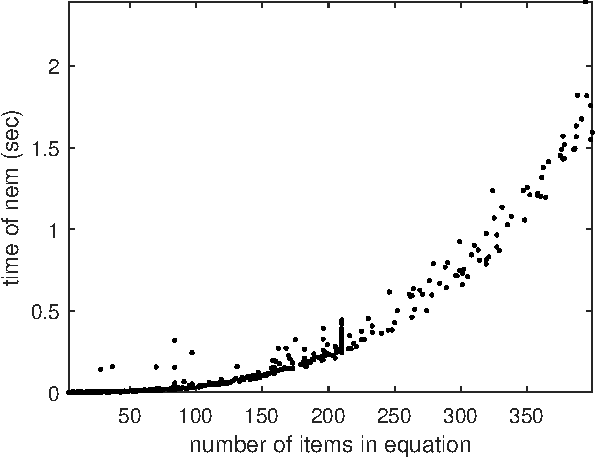
\includegraphics[width=.5\textwidth]{fig/t-nem.pdf}
\caption{NEM 的时间复杂度}
\label{t-nem}
\end{figure}

然后, 我们来关注平衡点类型的分布. 因为一共有三种平衡点, 所以我们用一个长度为3的二进制序列来表示一个方程的平衡点类型. 例如\cd{100}表示只有\BPone{}. 从\reffig{d-bps}可以看出, 几乎每个方程都有\BPone{}, 大部分方程在具有\BPone{}的同时还具有\BPthree{}. 在我们的测试中, 有2个方程只有\BPthree{}, 没有一个方程有\BPtwo{}. 这说明对于大部分的方程, 齐次平衡原则虽然能够直接求解, 但是不能排除漏解的可能性.


最后, 我们来关注一下方程的最小展开阶数. 方程的最小展开阶数指的是方程在展开后第一个非零系数出现的位置. 从\reffig{d-nExpand}中可以看出, 在我们的测试中, 只有2个例子需要二阶展开. 事实上, 这两个方程恰好是那两个只有\BPthree{}的方程. 这说明较小的展开阶数就能解决大部分的问题. 

\begin{figure}[htbp]
\centering
\subfigure[平衡点类型分布 \label{d-bps}]{
    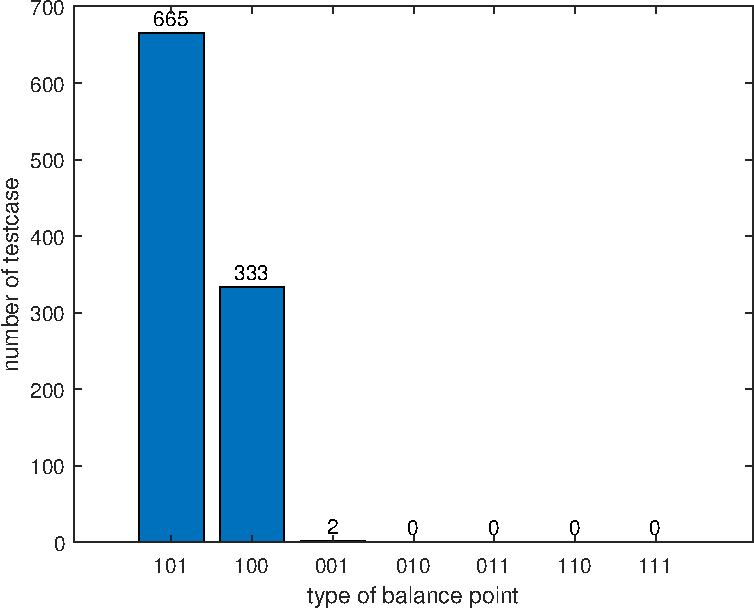
\includegraphics[width=0.45\textwidth]{fig/d-bpType.pdf}
}
\subfigure[最小展开阶数分布 \label{d-nExpand}]{
    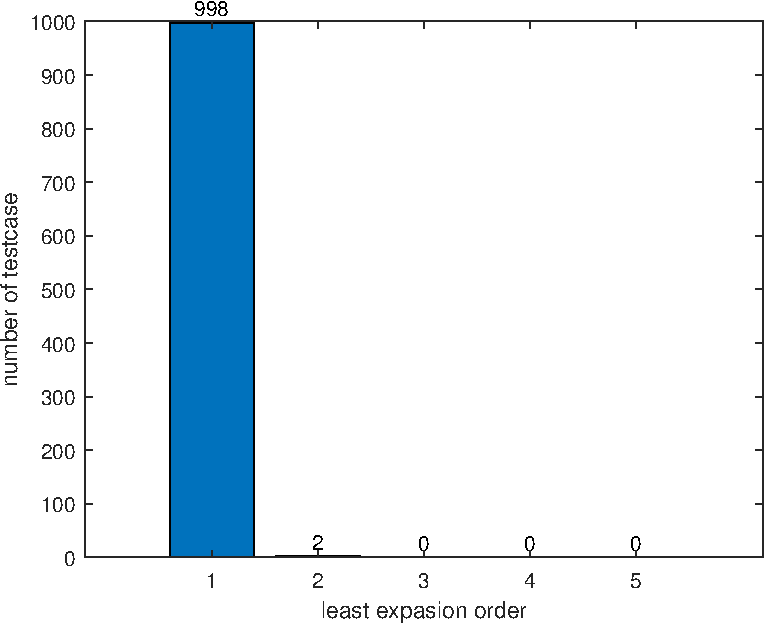
\includegraphics[width=0.45\textwidth]{fig/d-nExpand.pdf}
}
\caption{平衡点类型与最小展开阶数的分布图}
\end{figure}

\section{n阶展开方法在双曲正切方法中的应用}\label{ch4sec5}
和\refchp{ch02}一样, 双曲正切方法的求解对象也是非线性演化方程
\begin{equation}
    U\sbrace{u,u\up{1},u\up{2},\cdots}=0,
\end{equation}
其中 $u=u(x_1,\cdots,x_n)$, 而$U$则是关于$u$及其导数的多项式. 

在双曲正切方法中, 首先引入行波变换 
\begin{equation}
    \xi = p_1 x_1 +\cdots + p_n x_n + p_{n+1}.  \label{tanh-tw}
\end{equation}
根据链式求导法则可得
\begin{equation}
    \DIFF{u}{x_k}=\DIFF{u}{\xi}\DIFF{\xi}{x_k}=p_k\DIFF{u}{\xi}.
\end{equation}
基于上述行波变换, 可将原方程转化为关于$u(\xi)$的常微分方程
\begin{equation}
    V(u,u',u'',\cdots)=0. \label{odeq}
\end{equation}

接着, 假设\refeqnn{odeq}存在如下形式的解:
\begin{equation}
    u(\xi)=\sum_{k=0}^m{a_k \tanh^k(\xi)}. \label{tanh-poly}
\end{equation}
在原本的双曲正切方法中, 基于齐次平衡原则来确定$m$的上界. 现在, 我们可以基于$n$阶展开方法来完善它. 

和前文一样, 我们用$F(x,m,\mu\up{n})$来表示关于$x$的$m$次$n$阶展开多项式, 其最高$n$项的系数为$\mu\up{n}$. 于是, 可以将$u(\xi)$设为
\begin{equation}
    u(\xi)=F\sbrace{\tanh(\xi),m,\alpha\up{n}}.
\end{equation}

为了和解的假设形式保持一致, 我们取$\alpha\up{n}=[a_m,a_{m-1},\cdots,a_{m-n+1}]$, 即
\begin{equation}
    u(\xi)=a_m\tanh^m(\xi)+\cdots+a_{m-n+1}\tanh^{m-n+1}(\xi)+\OO\sbrace{\tanh^{m-n}(\xi)}.
\end{equation}

由\refeqn{NEM-diff}可知, 要使$u$关于$\xi$的导数也能表示为$n$阶展开多项式, 只需将$\DIF{\xi}\tanh(\xi)$表示为$n$阶展开多项式即可. 我们有 
\begin{equation}
    \DIFF{\tanh(\xi)}{\xi}=1-\tanh^2(\xi)=F\sbrace{\tanh(\xi),2,[-1,0,1]}.
\end{equation}
事实上, \cd{NEPoly}对象已经自动实现了上述转换. 将$u(\xi)$转化为\cd{NEPoly}对象之后, 代入\refeqnn{odeq}, 基于\cd{NEPoly}的微分和乘法操作将\refeqnn{odeq}的所有加法项转化为\cd{NEPoly}列表, 就能调用\cd{nem}求得平衡点的上界$\overline{m}$.

最后, 将$u(\xi)=\sum_{k=0}^{\overline{m}}{a_k \tanh^k(\xi)}$代入\refeqnn{odeq}就能求得原方程的双曲正切函数解.  此外, 我们在输出时还删除了平凡的解. 按照\refchp{ch03}的做法, 我们也对非平凡的双曲函数解定义了避免取值集合
\begin{equation}
    S=\bbrace{\bbrace{p_k=0}|1\le k \le n} \cup \bbrace{a_1=0,\cdots,a_m=0}.
\end{equation}
式中第一个集合保证解的维数不会退化, 第二个集合保证解不是常数. 

基于上述过程, 我们实现了 NCTM 软件包. NCTM 的核心接口为
\begin{verbatim}
sh:=nctm(eq,a,p,{SP,nExpand});
\end{verbatim}
其中
\begin{compactitem}[\textbullet]
\item \cd{eq} 表示输入的方程.
\item \cd{a} 表示\refeqn{tanh-poly}中的待定系数的变量名.
\item \cd{p} 可以是一个变量名, 也可是一个变量名列表, 用于指定\refeqn{tanh-tw}中行波变换的系数.
\item 可选参数\cd{SP}表示方程中可以求解的参数. 因为对于一些带参方程, 有时需要探索方程是否在某些参数条件下有解.
\item 可选参数\cd{nExpand}表示$n$阶展开的阶数, 默认值为2.
\item 返回结果\cd{sh}是一个\cd{SolHolder}对象, 它和TwSolver中的\cd{SolHolder}对象一样, 提供了获取解的表达式\D 验证解和绘制解等功能. 
\end{compactitem}

接下来, 我们用几个典型的例子来展示 NCTM 的基本用法, 以及它相对于现有双曲正切函数法的软件包的改进. 在\refchp{ch01}中, 我们介绍了许多关于双曲正切方法的机械化工作. 其中 从 Maple 9.5 开始引入的 \cd{PDEtools:-TWSolutions} 函数兼容性好, 能够求解高维的方程, 所以我们主要以它为例进行比较. 

\begin{example}含全部三类平衡点, 同时用于介绍NCTM的基本用法. 

虽然现有的双曲正切方法能够在只考虑第一类平衡点的情况下完成求解, 但是只要有阶数相同的最高项存在, 就不能排除另外两类平衡点存在的可能性. 但是, 基于$n$阶展开方法就能排除漏解的可能性, (4+1)维 Fokas方程就是一个典型的例子. 对于(4+1)维 Fokas方程\CITEdaFokas{}
\begin{equation}
    u_{tx}-\frac{1}{4}u_{xxxy}+\frac{1}{4}u_{xyyy}+3u_xu_y+3uu_{xy}-\frac{3}{2}u_{wz}=0 ,
\end{equation}
其阶数列表为$\mbrace{2m+2,m+4,m+4,2m+2,m+2}$. 
\begin{compactitem}[\textbullet]
\item 首先, 根据最大性约束, 可以将阶数列表简化为$\mbrace{2m+2,m+4,m+4,2m+2}$.
\item 接着, 考虑第一类平衡点. 根据$2m+2=m+4$可以得到第一类平衡点$m=2$.
\item 然后, 考虑第二类平衡点. 从$m+4=m+4$出发, 根据最大性约束有$m+4>2m+2$, 可得$m<2$, 所以有第二类平衡点$m=1$.
\item 最后, 因为有两个$2m+2$, 所以需要考虑第三类平衡点. 作行波变换$\xi=kx+py+qz+rw+ct+\eta$, 将$u$的2阶展开形式$u(\xi)=a_m\tanh^m(\xi)+a_{m-1}\tanh^{m-1}(\xi)+\OO\sbrace{\tanh^{m-2}(\xi)}$代入变换后的方程, 可以将方程重写为2阶展开的形式
\begin{equation}
\begin{aligned}
0&=24kpa_m^2m\sbrace{m+\frac{1}{2}}\tanh^{2m+2}(\xi)\\ 
&+24\,k\,p\,{{a}_{m}}\,{{a}_{m-1}}\,m\,\left( 2\,m-1\right)\tanh^{2m+1}(\xi)+\OO\sbrace{\tanh^{2m}(\xi)} . 
\end{aligned}
\end{equation}
因为$\Omega_0=24kpa_m^2m\sbrace{m+\frac{1}{2}}=0$关于$m$没有正整数解, 所以需要$2m+2-0\le m+4$, 从而得到第三类平衡点的上界为$m=2$.
\end{compactitem}
   
最终, 我们确定$m=2$, 这既是第一类平衡点, 也是第三类平衡点. 调用
\begin{verbatim}
sh:=nctm(eq,a,[k,p,q,r,eta])
\end{verbatim}
将会自动进行上述分析, 并得出原方程有解
\begin{equation}
    u=a_0 +a_1 \tanh(\xi) + a_2 \tanh^2(\xi), 
\end{equation}
其中 $\xi=kx+py+qz+rw+ct+\eta$, 且
\begin{equation}
    \left\{ {{a}_{0}}=\frac{\left( -4\,{k}^{3}\,p+4\,k\,{p}^{3}-2\,c\,k+3\,q\,r\right) }{6\,p\,k},{{a}_{1}}=0,{{a}_{2}}={k}^{2}-{p}^{2}\right\} . \label{nctm-fokas-sol}
\end{equation}

\cd{ntcm}函数的返回值\cd{sh}也是一个\cd{SolHolder}对象, 它提供了计算\D 验证和绘制解的功能. 
\begin{compactitem}[\textbullet]
\item \cd{sh:-get\_sols()}将会返回原方程对应的代数方程组的所有解. 在这个例子中, 调用 \cd{sh:-get\_sols()[1]}就能得到\refeqn{nctm-fokas-sol}.
\item \cd{sh:-get\_sol(s)}会将参数关系\cd{s}代入到解的假设形式中, 并返回解的表达式. 在这个例子中, 设\cd{s}为\refeqn{nctm-fokas-sol}, 调用\cd{sh:-get\_sol(s)}将会得到 
\begin{equation}
\begin{aligned}
u&=\frac{\left( -4\,{k}^{3}\,p+4\,k\,{p}^{3}-2\,c\,k+3\,q\,r\right) }{6\,p\,k} \\
&+\left( {k}^{2}-{p}^{2}\right) \,\tanh^2\left( c\,t+k\,x+p\,y+q\,z+r\,w+\eta\right) . 
\label{nctm-long-sol}
\end{aligned}  
\end{equation}
\item 因为\refeqn{nctm-long-sol}的结果较长, \cd{sh}还提供了获得解的简写形式的接口\cd{get\_short\_sol}, 其结果为 
\begin{equation}
\begin{aligned}
u&=\left( {k}^{2}-{p}^{2}\right) \,{T}^{2}+\frac{\left( -4\,{k}^{3}\,p+4\,k\,{p}^{3}-2\,c\,k+3\,q\,r\right) }{6\,p\,k}, \\
T&=\tanh\left( c\,t+k\,x+p\,y+q\,z+r\,w+\eta\right) . 
\end{aligned}
\end{equation}
\item \cd{sh:-verify\_sol(s)}将会验证由\cd{sh:-get\_sol(s)}得到的解是否满足原方程.
\item \cd{sh:-plot\_sol}可以绘制解的图像, 其接口类似于 TwSolver 和 NS1L 中的绘制接口, 都提供了参数默认赋值和兼容\cd{plot3d}附加参数的功能. 例如调用
\begin{verbatim}
sh:-plot_sol(sol,[x=-20..20,y=-20..20,z=0,w=0,t=0,k=1/4]
\end{verbatim}
将会得到如\reffig{tanh-fokas}所示的结果.
\end{compactitem}
\begin{figure}[h]
\centering
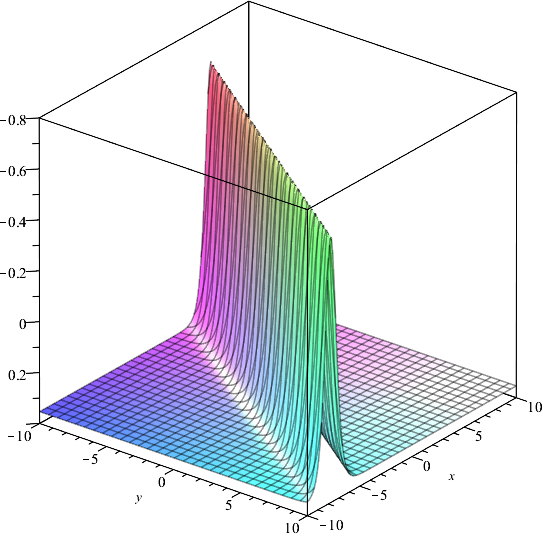
\includegraphics[width=.5\textwidth]{fig/(4+1)Fokas-tanh.png}
\caption{(4+1)维Fokas方程的双曲正切函数解} \label{tanh-fokas}
\end{figure}

在这个例子中, 调用\cd{PDEtools:-TWSolutions}也能得到相同的解. 尽管第三类平衡点并没有起到决定性的作用, 但是我们利用$n$阶展开方法排除了其它解存在的可能性.
\end{example}

\begin{example} 第三类平衡点的主导作用 

考虑方程 \cite{EMM}
\begin{equation}
    {{u}_{t}}+{{u}_{x}}+\alpha\,{{u}_{xxx}}+\beta\,u\,{{u}_{x}}+\gamma\,u\,{{u}_{xxx}}+\delta\,{{u}_{x}}\,{{u}_{xx}}=0,
\end{equation}
这是一个从弹性介质的微观结构(Elastic Media with Microstructure)中导出的非线性演化方程, 所以我们称它为(1+1)维EMM方程. 取$\xi=kx+ct+\eta$, 调用 \cd{nctm(eq,a,[k,c,eta])} 进行求解, 可得其阶数列表为$[m+1,m+1,m+3,2m+1,2m+3,2m+3]$. 由
\begin{equation}
    \Omega_0=-{{{a}_{m}}}^{2}\,{k}^{3}\,m\,\left( m+1\right) \,\left( m\,\delta+\gamma\,m+2\,\gamma\right)
\end{equation}
可得 $m=0$, 原方程没有非平凡的解. 当$m=\frac{-2 \gamma}{\gamma+\delta}$为正整数时, 就存在其它可能的平衡点.  事实上, NCTM 能够发现此类情况并输出警告. 

当$\gamma=-1,\delta=3$时, $m=1$, 原方程有两个解 
\begin{equation}
u=\alpha+{{a}_{1}}\,\tanh\left(\pm\sbrace{\frac{\sqrt {\beta}\,\left( \alpha\,\beta+1\right)}{2}t-\frac{\sqrt {\beta}}{2}x}+\eta\right) . \label{emm-tanh-1}
\end{equation}

此外, 我们总结出: 当$n\ge 1$时, 若$\gamma=-n,\delta=n+1$, 则$m=2n$, 原方程有解
\begin{equation}
u=a_{2n} \sbrace{1-\tanh^2\sbrace{\pm\sbrace{\frac{\sqrt{-\beta}}{2n}x-\frac{\sqrt{-\beta}(\alpha\beta+n)}{2n^2}t}+\eta}}^n+\frac{\alpha}{n} . \label{emm-tanh-n}
\end{equation}

对于\refeqn{emm-tanh-n}所表示的解, 我们取$\bbrace{a_{2n}=1,\alpha=1,\beta=-1,\eta=0}$进行绘图, 当$n=1,2,3$时, 其图像如\reffig{emm-tanh}所示. 
\begin{figure}[ht]
\centering
\subfigure[$n=1$]{
    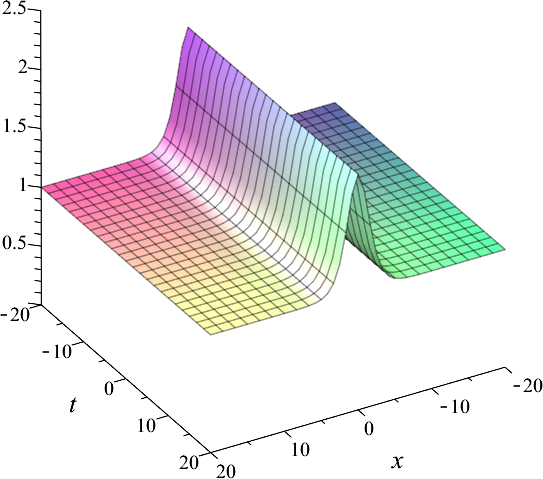
\includegraphics[width=.3\textwidth]{fig/(1+1)EMM-tanh-1.png}
}
\subfigure[$n=2$]{
    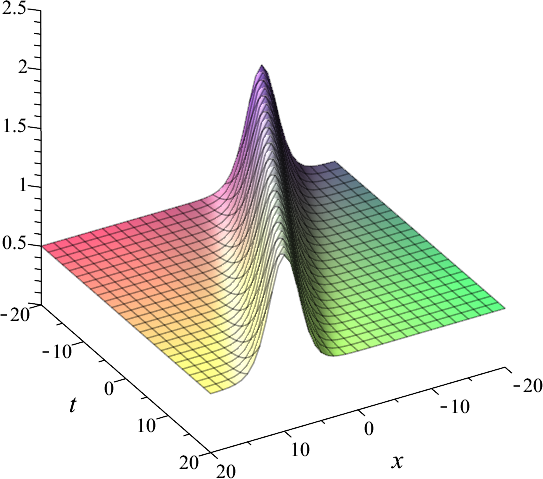
\includegraphics[width=.3\textwidth]{fig/(1+1)EMM-tanh-2.png}
}
\subfigure[$n=3$]{
    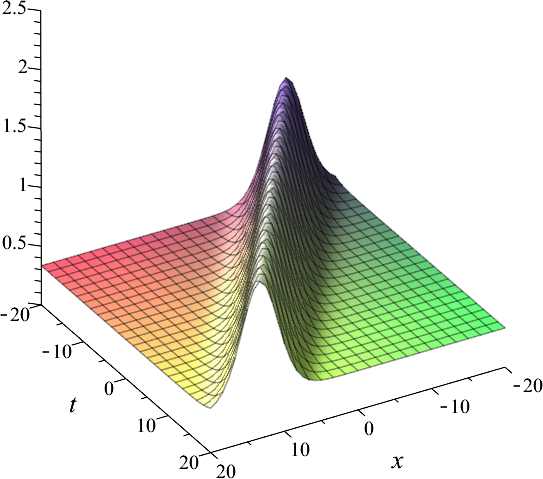
\includegraphics[width=.3\textwidth]{fig/(1+1)EMM-tanh-3.png}
}
\caption{(1+1)维EMM方程的双曲正切函数解} \label{emm-tanh}
\end{figure}

对于这个例子, 采用\cd{PDEtools:-TWSolutions}进行求解的结果如下: 
\begin{compactitem}[\textbullet]
\item 若直接求解原方程, 将无法得到非平凡的解.
\item 取$\gamma=-1,\delta=3$, 虽然不能通过齐次平衡原则确定$m$的值, 但是\cd{TWSolutions}将会取$m=3$进行求解, 从而得到和\refeqn{emm-tanh-1}相同的两个解. 
\item 取$\gamma=-n,\delta=n+1$进行求解, 由于\cd{PDEtools:-TWSolutions}会按$m=3$进行求解, 所以只能在$n=1$时得到解. 
\end{compactitem}

因此, 这个例子充分展示了用$n$阶展开方法完善齐次平衡原则的必要性和有效性.
\end{example}

\begin{example}同时存在多个不同次数的解

尽管在我们的方法中, 取$m=\overline{m}$在理论上能够求得所有次数不超过$\overline{m}$的解, 但是大多数方程只存在$m=\overline{m}$的解, 即只有一个平衡点是有解的. 而这个例子则展示了同时存在多个不同次数的解的情况.

考虑一般五阶模型\cite{kichenassamy1992existence}
\begin{equation}
    u_t+\sbrace{\alpha\,u_x^2+\beta\,u\,{{u}_{xx}}+\mu\,{{u}_{xx}}+{{u}_{xxxx}}+p\,u+q\,{u}^{2}+r\,{u}^{3} }_x = 0. 
\end{equation}
当$\alpha=5,\beta=-4,r=0$时, 则其阶数列表为$[m+1,2m+3,2m+3,m+3,m+5,m+1,2m+1]$. 由最大性条件, 上述列表可简化为$\mbrace{2m+3,2m+3,m+5}$.

首先, 考虑第一类平衡点, 由$2m+3=m+5$可得$m=2$.

然后, 考虑第三类平衡点, 取$\xi=kx+ct+\eta$, 我们有 
\[
    \Omega_0 = -2k^3a_m^2m(m+1)(m-4) .
\]
$\Omega_0=0$有正整数解$m=4$.

综上, 我们取$m=4$进行求解, 可以得到原方程的两个解:
\begin{equation}
\begin{aligned}
u&=30\,{k}^{2}\,{T}^{2}-20\,{k}^{2}+\frac{\mu}{4}+\frac{5\,q}{4}, \\
T&=\tanh\left( \frac{k\,\left( 288\,{k}^{4}-\mu\,q-5\,{q}^{2}-2\,p\right) \,t}{2}+k\,x+\eta\right),
\end{aligned}
\end{equation}
和
\begin{equation}
\begin{aligned}
u&=\frac{{-3360\,{k}^{4}\,{T}^{4}+6720\,{k}^{4}\,{T}^{2}-2528\,{k}^{4}+16\,{k}^{2}\,\mu+52\,{k}^{2}\,q+\mu\,q}}{64\,{k}^{2}+4\,q} ,\\ 
T&=\tanh\left( \frac{k\,\left( 1152\,{k}^{4}-52\,{k}^{2}\,q-\mu\,q-2\,p\right) \,t}{2}+k\,x+\eta\right) .
\end{aligned}
\end{equation}

值得注意的是, $m=2$的解是由第一类平衡点得到的, $m=4$的解是由第三类平衡点得到的. 采用\cd{PDEtools:-TWSolutions}只能得到$m=2$的解. 
    
\end{example}

对于一些带参数的方程, 有时需要探索方程是否在某些参数条件下有解. 所以我们将在下一个例子中展示参数\cd{SP}的作用.

\begin{example}可以求解出相应的参数约束条件. 

对于(1+1)维 7阶色散方程\cite{duffy1996travelling}
\begin{equation}
    {{u}_{t}}+u\,{{u}_{x}}+p\,{{u}_{3x}}+q\,{{u}_{5x}}+r\,{{u}_{7x}}=0,
\end{equation}
设$\xi=kx+ct+\eta$. 若调用
\begin{verbatim}
nctm(eq,a,[k,c,eta]);
\end{verbatim}
则无解. 此时, 我们允许参数$r$被其它参数表示, 调用
\begin{verbatim}
nctm(eq,a,[k,c,eta],SP={r});
\end{verbatim}
可以确定$m=6$, 并得到6个解:
\begin{equation}
\renewcommand{\arraystretch}{1.4}
\begin{array}{rl}
r=0:& u=\pm \frac{2\,q\,\sqrt {13}\,c}{\sqrt {-p\,q}}-\frac{3\,{p}^{2}\,\left( 35\,{T}^{4}-70\,{T}^{2}+23\right) }{169\,q},k=-\frac{\sqrt {13}\,\sqrt {-p\,q}}{26\,q};\\
r=\frac{769 q^2}{2500 p}:& u=\frac{1538\,c\,q\,k}{25\,p}+\frac{2250\,{p}^{2}\,\left( 231\,{T}^{6}-693\,{T}^{4}+693\,{T}^{2}-151\right) }{591361\,q},k=\pm \frac{5\,\sqrt {1538}\,\sqrt {-p\,q}}{1538\,q};\\
r=\frac{2519 q^2}{10000 p}:& u=\frac{2159\,c\,q\,k}{25\,p}+\frac{500\,{p}^{2}\,\left( 2079\,{T}^{6}-8316\,{T}^{4}+10395\,{T}^{2}-2738\right) }{4661281\,q},k=\pm\frac{5\,\sqrt {2159}\,\sqrt {-p\,q}}{2159\,q}, \\
\end{array}
\end{equation}
其中 $T=\tanh\sbrace{kx+ct+\eta}$. 

因为\cd{PDEtools:-TWSolutions} 不支持对参数进行求解, 所以我们将此结果和 RATH 进行比较. 即使删去$r=0$时的两个解, 我们的解依然比 RATH\cite[p21]{liu2001master} 丰富, 因为 RATH 只给出了$r=\frac{769 q^2}{2500 p}$和$r=\frac{2519 q^2}{10000 p}$时的两个解. 
\end{example}

\section{n阶展开方法在\Painleve{}展开法中的应用}\label{ch4sec6}
在\Painleve{}展开法中, 假设 
\begin{equation}
    u=\sum_{k=1}^{m}\frac{u_k}{f^{m-k+1}}. \label{TPE-pkg}
\end{equation}
我们可以将其看作是关于$1/f$的多项式
\begin{equation}
    u=F\sbrace{\frac{1}{f},m,\mu\up{n}}.
\end{equation}
在应用$n$阶展开方法时, 因为 
\begin{equation}
    \DIF{x}{\frac{1}{f}}=-\frac{f_x}{f^2}=F\sbrace{\frac{1}{f},2,\mbrace{-f_x,0,0}},
\end{equation}
也能根据\refeqn{NEM-diff}完成求导操作. 

在将$u$及其导数转化为关于$1/f$的$n$阶展开多项式之后, 利用\cd{NEPoly}对象的乘法操作, 可以将原方程的各个加法项也转化为\cd{NEPoly}对象. 然后, 我们就可以利用\cd{nem}来分析$m$的上界. 之后, 我们就可以将\refeqn{TPE-pkg}代入原方程, 利用\refalg{rpsolve}实现待定系数的求解. 对于\refalg{rpsolve}的求解结果, 我们会删去全零的解. 最终, 我们将返回输入方程的 TPE. 

基于上述方法, 我们实现了 PExpand 软件包. PExpand 的核心接口为
\begin{verbatim}
ftr:=panalyze(eq,u,f,{nExpand,selelct_solution});
\end{verbatim}
其中
\begin{compactitem}[\textbullet]
\item \cd{eq}表示输入的方程, \cd{u}表示方程中的未知函数, \cd{f}表示变换后的未知函数, 要求\cd{u}和\cd{f}拥有相同的自变量.
\item 可选参数\cd{nExpand}表示$n$阶展开的阶数, 默认值为2.
\item 可选参数\cd{select\_solution}的作用和\cd{twsolve}中的同名参数一样, 用于允许用户通过交互的方式选择解. 如果不指定该参数, 函数将默认返回第一个解. 
\item 返回值\cd{ftr}表示形如\refeqn{TPE-pkg}的TPE. 
\end{compactitem}

下面以一个典型的例子来展示 NEM 在\Painleve{}展开法中的应用.

\begin{example}
考虑方程
\begin{equation}
    u(u_t+u_{xxx})-3u_x u_{xx}=0. \label{pseq}
\end{equation}
其阶数列表为$\mbrace{2m+1,2m+3,2m+3}$, 只有\BPthree{}. 由
\begin{equation}
    \Omega_0=2m(m^2-1)u_0^2f_x^3
\end{equation}
可得$m=1$. 将$u=\mu/f$代入原方程后, 关于$1/f$的最高项系数为
\begin{equation}
    3\,\mu\,{{f}_{x}}\,\left( \mu\,{{f}_{xx}}-2\,{{\mu}_{x}}\,{{f}_{x}}\right) .
\end{equation}
可以解得 
\begin{equation}
    \mu=F(t)\sqrt{f_x}.
\end{equation}
\end{example}
我们取$\mu=\sqrt{f_x}$, 即$u=\sqrt{f_x}/f$代入\refeqnn{pseq}, 可以得到
\begin{equation}
\begin{aligned}
& 2\,{{f}_{tx}}\,{{{f}_{x}}}^{2}\,f+2\,{{f}_{xxxx}}\,{{{f}_{x}}}^{2}\,f-6\,{{f}_{xx}}\,{{f}_{xxx}}\,{{f}_{x}}\,f+3\,{{{f}_{xx}}}^{3}\,f \\
-&4\,{{{f}_{x}}}^{3}\,{{f}_{t}}-4\,{{f}_{xxx}}\,{{{f}_{x}}}^{3}+6\,{{{f}_{xx}}}^{2}\,{{{f}_{x}}}^{2}=0.
\end{aligned} \label{pseq-f}
\end{equation}
随后, 我们就能基于\refeqnn{pseq-f}进行各种类型的解的求解.

事实上, 本文所实现的 PExpand 软件包能够自动导出变换$u=F(t)\sqrt{f_x}/f$, 但是我们不能以这个变换为基础进行后续的求解.  因此, 本文实现的 TwSolver 和 NS1L 都不能直接求解\refeqnn{raeq}. 但是, 这两个软件包都提供了自定义变换进行求解的功能.

在TwSolver中, 调用
\begin{verbatim}
twsolve(
    eq,{1},PL=[k,c],
    _utr=(f->sqrt(diff(f,x))/f)
);
\end{verbatim}
就能够指定变换进行求解. 该方程在简单Hirota方法下只有1-孤子解
\begin{equation}
    f=1+\exp\sbrace{k\sbrace{x+\frac{k^2}{2}t}+c}.
\end{equation}
在NS1L中, 也可以利用参数\cd{\_utr=(f->sqrt(diff(f,x))/f)}指定变换进行求解. 不过, 该方程没有lump解.

\begin{example} 
考虑方程 \cite{EMM}
\begin{equation}
    {{u}_{t}}+{{u}_{x}}+\alpha\,{{u}_{xxx}}+\beta\,u\,{{u}_{x}}+\gamma\,u\,{{u}_{xxx}}+\delta\,{{u}_{x}}\,{{u}_{xx}}=0,
\end{equation}
其阶数列表为$[m+1,m+1,2m+1,2m+3,2m+3]$, 只有第三类平衡点. 对该方程进行1阶展开, 即取$u=\mu_0/f^m+\OO(1/f^{m-1})$代入原方程, 可以得到
\begin{equation}
    -\mu_0^2f_x^3m(m+1)(\gamma m+\delta m+2\gamma)\frac{1}{f^{2m+3}}+\OO\sbrace{\frac{1}{f^{2m+2}}}=0. 
\end{equation}
当$\gamma=-1,\delta=3$时, $m=1$, PExpand 可以解得 
\begin{equation}
    u=\frac{\sqrt{f_x}}{f}\sbrace{\alpha\int\!{\sqrt{f_x}{\,\rm d}x}+F(t)}.
\end{equation}
而其它软件只能得到$m=0$, 从而无法继续求解. 
\end{example}

\section{小结}\label{ch4sec7}

在本章中, 我们提出了$n$阶展开方法来完善齐次平衡原则, 并将其应用于微分方程和差分方程的若干求解方法中. 我们针对$n$阶展开方法开发了 NEM 软件包, 并在此基础上开发了求解非线性差分方程多项式解的软件包NLREPS. 同时, 我们还将$n$阶展开方法应用于微分方程的求解. 我们开发了基于双曲正切方法的 NCTM 和实现\Painleve{}展开法的 PExpand. 

实验和例子表明, $n$阶展开方法确实完善了齐次平衡原则, 能更加全面的分析平衡的情况, 在求解时获得更多的解. 此外, 对于大部分的方程, 展开阶数为2已经能够完成求解. 

% 本章的成果已被华东师范大学学报(自然科学版)接受.

\chapter{$n$阶展开方法在微分方程求解中的应用}\label{ch05}
在上一章中, 为了完善齐次平衡原则, 我们提出了$n$阶展开方法, 并将其应用于非线性差分方程的求解. 在这一章中, 我们将以双曲正切方法和\Painleve{}分析为例, 展示$n$阶展开方法在微分方程求解中的应用.

\section{$n$阶展开方法在双曲正切方法中的应用}
和\refchp{ch02}一样, 双曲正切方法的求解对象也是非线性演化方程
\begin{equation}
    U\sbrace{u,u\up{1},u\up{2},\cdots}=0,
\end{equation}
其中, $u=u(x_1,\cdots,x_n)$, 而$U$则是关于$u$及其导数的多项式. 

在双曲正切方法中, 我们首先取行波变换 
\begin{equation}
    \xi = p_1 x_1 +\cdots + p_n x_n + p_{n+1}.  \label{tanh-tw}
\end{equation}
根据链式求导法则, 我们有,
\begin{equation}
    \DIFF{u}{x_k}=\DIFF{u}{\xi}\DIFF{\xi}{x_k}=p_k\DIFF{u}{\xi}.
\end{equation}
基于上述行波变换, 我们可以将原方程转化为关于$u(\xi)$的常微分方程
\begin{equation}
    V(u,u',u'',\cdots)=0. \label{odeq}
\end{equation}

接着, 我们假设\refeqnn{odeq}存在如下形式的解:
\begin{equation}
    u(\xi)=\sum_{k=0}^m{a_k \tanh^k(\xi)}. \label{tanh-poly}
\end{equation}
在原本的双曲正切方法中, 我们基于齐次平衡原则来确定$m$的上界. 现在, 我们可以基于$n$阶展开方法来完善它. 

和\refchp{ch04}一样, 我们用$F(x,m,\mu\up{n})$来表示关于$x$的$m$次$n$阶展开多项式, 其最高$n$项的系数为$\mu\up{n}$. 于是, 我们可以将$u(\xi)$设为
\begin{equation}
    u(\xi)=F\sbrace{\tanh(\xi),m,\alpha\up{n}}.
\end{equation}

由\refeqn{NEM-diff}可知, 要使$u$的关于$\xi$导数也能表示为$n$阶展开多项式, 只需将$\DIF{\xi}\tanh(\xi)$表示为$n$阶展开多项式即可. 我们有 
\begin{equation}
    \DIFF{\tanh(\xi)}{\xi}=1-\tanh^2(\xi)=F\sbrace{\tanh(\xi),2,[-1,0,1]}.
\end{equation}
事实上, \cd{NEPoly}对象已经自动实现了上述转换. 将$u(\xi)$转化为\cd{NEPoly}对象之后, 代入\refeqnn{odeq}, 基于\cd{NEPoly}的微分和乘法操作将\refeqnn{odeq}的所有加法项转化为\cd{NEPoly}列表, 就能调用\cd{nem}求得平衡点的上界$\overline{m}$.

最后, 将$u(\xi)=\sum_{k=0}^{\overline{m}}{a_k \tanh^k(\xi)}$代入\refeqnn{odeq}就能求得原方程的双曲正切函数解.  此外, 我们在输出时还删除了平凡的解. 按照\refchp{ch03}的做法, 我们也对非平凡的双曲函数解定义了避免取值集合
\begin{equation}
    S=\bbrace{\bbrace{p_k=0}|1\le k \le n} \cup \bbrace{a_1=0,\cdots,a_m=0}.
\end{equation}
式中第一个集合保证解的维数不会退化, 第二个集合保证解不是常数. 

基于上述过程, 我们实现了 NCTM 软件包. NCTM 的核心接口为
\begin{verbatim}
sh:=nctm(eq,a,p,{SP,nExpand});
\end{verbatim}
其中,
\begin{compactitem}[\textbullet]
\item \cd{eq} 是输入的方程.
\item \cd{a} 是\refeqn{tanh-poly}中的待定系数的变量名.
\item \cd{p} 可以是一个变量名, 也可以是一个变量名的列表, 用于指定\refeqn{tanh-tw}中行波变换的系数.
\item 可选参数\cd{SP}表示方程中可以求解的参数. 因为对于一些带参数的方程, 我们有时需要探索方程是否在某些参数条件下有解.
\item 可选参数\cd{nExpand}表示$n$阶展开的阶数, 默认值为2.
\item 返回结果\cd{sh}是一个\cd{SolHolder}对象, 它和TwSolver中的\cd{SolHolder}对象一样, 提供了获取解的表达式\D 验证解和绘制解等功能. 
\end{compactitem}

接下来, 我们用几个典型的例子来展示 NCTM 的基本用法, 以及它相对于现有双曲正切函数法的软件包的改进. 

\begin{example}(1+1)Fisher 方程, 用于展示基本用法.

考虑(1+1)Fisher 方程\cite{guo1991analytic},
\begin{equation}
    u_t-u_{x,x}-u(1-u)=0.
\end{equation}
我们取行波变换$\xi=kx+ct+\eta$, 则调用语句为
\begin{verbatim}
sh:=ntcm(eq,a,[k,c,eta]);
\end{verbatim}
最终, NCTM确定$m=2$, 从而确定解的假设形式为 
\begin{eqnarray}
    u(\xi)=a_0+a_1 \tanh(\xi)+a_2\tanh^2(\xi).
\end{eqnarray}
通过求解对应的代数方程组, \cd{NTCM}得到了4个解. 调用 
\begin{verbatim}
sols:=sh:-get_sols()
\end{verbatim}
可以返回 4 组参数关系
\begin{equation}
    \bbrace{a_0=a_2=\frac{1}{4},a_1=\pm \frac{1}{2},k=\pm \frac{\sqrt 6}{12},c=\frac{5}{6}a_1}. \label{para-rel}
\end{equation}
相比于RATH\cite[p35]{liu2001master}中的两个解, \cd{NTCM}的解更加全面.

如果想要获取解的表达式, 则可以调用\cd{sh:-get\_sol}. 在这个例子中, 调用
\begin{verbatim}
sh:-get_sol(sols[4]);
\end{verbatim}
可以得到
\begin{equation}
    u(x,t)=\frac{1}{4}\sbrace{1+2\tanh\sbrace{\frac{1}{12}(\sqrt{6}x+5t)+\eta}+\tanh^2\sbrace{\frac{1}{12}(\sqrt{6}x+5t)+\eta}}. \label{fisher-sol-4}
\end{equation}

如果用户想验证所得的解是否满足原方程, 则可以调用
\begin{verbatim}
sh:-verify_sol(sol);
\end{verbatim}
其中, \cd{sol}是一个参数关系的集合.

最后, 用户还能对所得的解进行绘图. 在这个例子中, 调用
\begin{verbatim}
sh:-plot_sol(sols[4],[x=-10..10,t=-10..20,eta=-2],rest_assign);
\end{verbatim}
可以得到如图\reffig{fisher-tanh}所示的结果. 这是\refeqn{fisher-sol-4}在取$\eta=-2$时的绘图结果. 
    
\end{example}

对于一些带参数的方程, 我们有时需要探索方程是否在某些参数条件下有解. 所以我们将在下一个例子中展示参数\cd{SP}的作用.

\begin{example}允许求解方程参数

对于(1+1)7阶色散方程\cite{duffy1996travelling}
\begin{equation}
    {{u}_{t}}+u\,{{u}_{x}}+p\,{{u}_{3x}}+q\,{{u}_{5x}}+r\,{{u}_{7x}}=0,
\end{equation}
我们设$\xi=kx+ct+\eta$. 若调用
\begin{verbatim}
ntcm(eq,a,[k,c,eta]);
\end{verbatim}
则无解. 此时, 我们允许参数$r$被其它参数表示, 调用
\begin{verbatim}
ntcm(eq,a,[k,c,eta],SP={r});
\end{verbatim}
可以确定$m=6$, 并得到6个解:
\begin{equation}
\def\arraystretch{1.2}
\begin{array}{rl}
r=0:& u=\pm \frac{2\,q\,\sqrt {13}\,c}{\sqrt {-p\,q}}-\frac{3\,{p}^{2}\,\left( 35\,{T}^{4}-70\,{T}^{2}+23\right) }{169\,q},k=-\frac{\sqrt {13}\,\sqrt {-p\,q}}{26\,q};\\
r=\frac{769 q^2}{2500 p}:& u=\frac{1538\,c\,q\,k}{25\,p}+\frac{2250\,{p}^{2}\,\left( 231\,{T}^{6}-693\,{T}^{4}+693\,{T}^{2}-151\right) }{591361\,q},k=\pm \frac{5\,\sqrt {1538}\,\sqrt {-p\,q}}{1538\,q};\\
r=\frac{2519 q^2}{10000 p}:& u=\frac{2159\,c\,q\,k}{25\,p}+\frac{500\,{p}^{2}\,\left( 2079\,{T}^{6}-8316\,{T}^{4}+10395\,{T}^{2}-2738\right) }{4661281\,q},k=\pm\frac{5\,\sqrt {2159}\,\sqrt {-p\,q}}{2159\,q}.\\
\end{array}
\end{equation}
其中, $T=\tanh\sbrace{=kx+ct+\eta}$. 

即使删去$r=0$时的两个解, 我们的解依然比 RATH\cite[p21]{liu2001master} 丰富, 因为RATH只给出了$r=\frac{769 q^2}{2500 p}$和$r=\frac{2519 q^2}{10000 p}$时的两个解.
\end{example}

\begin{figure}[htbp]
\centering
\subfigure[(1+1)Fisher\label{fisher-tanh}]{
    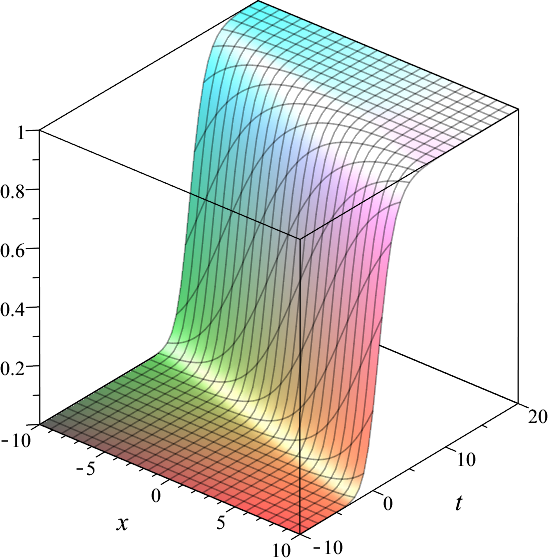
\includegraphics[width=.45\textwidth]{fig/(1+1)Fisher-tanh.png}
}
\subfigure[(2+1)KP\label{kp2-tanh}]{
    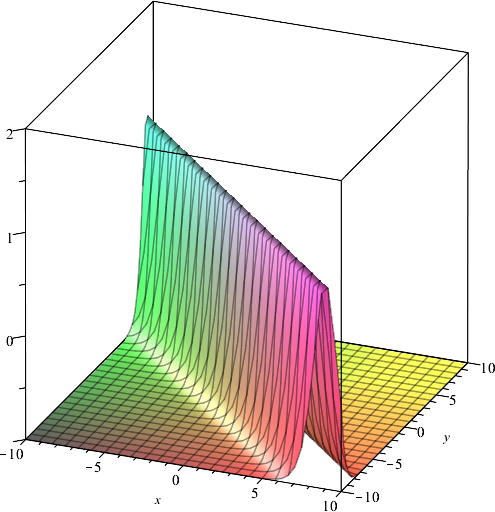
\includegraphics[width=.45\textwidth]{fig/(2+1)KP-tanh.png}
}
\subfigure[(3+1)KP\label{kp3-tanh}]{
    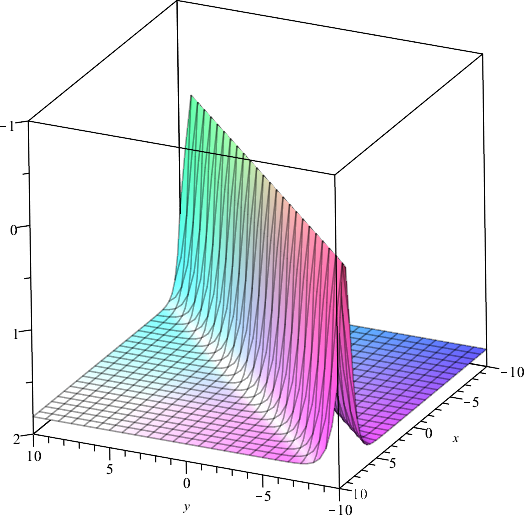
\includegraphics[width=.45\textwidth]{fig/(3+1)KP-tanh.png}
}
\subfigure[(4+1)Fokas\label{fokas-tanh}]{
    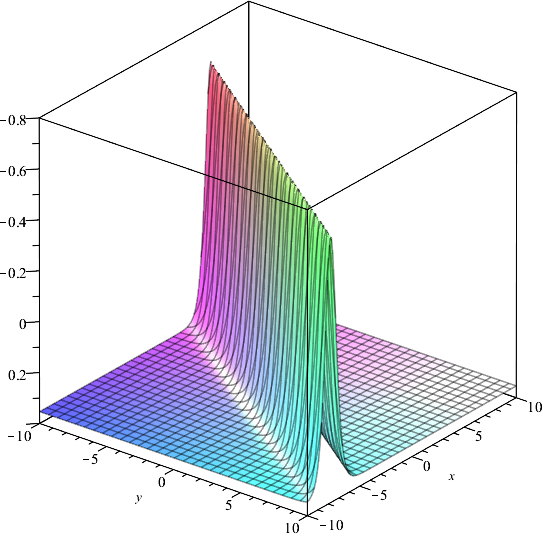
\includegraphics[width=.45\textwidth]{fig/(4+1)Fokas-tanh.png}
}
\caption{一些方程的双曲函数解}
\end{figure}

在以往的双曲正切方法中, 我们主要求解(1+1)维的方程. 而\cd{NTCM}实现了任意维度的行波变换, 所以能够求解更高维度的方程. 现给出几个典型的例子.

\begin{example}(2+1)KP方程\CITEbaKP{}

对于
\begin{equation}
    \alpha\,u_{{{\it yy}}}+6\,uu_{{{\it xx}}}+6\,{u_{{x}}}^{2}+u_{{{\it tx}}}+u_{{{\it xxxx}}}=0,
\end{equation}
我们取$\xi=kx+py+ct+\eta$. \cd{NTCM}确定$m=2$, 并给出了一个解
\begin{equation}
    \left\{ {{a}_{0}}=\frac{\left( 8\,{k}^{4}-\alpha\,{p}^{2}-k\,c\right) }{6\,{k}^{2}},{{a}_{1}}=0,{{a}_{2}}=-2\,{k}^{2}\right\} .
\end{equation}
取$\alpha=k=c=1=\eta=1,t=0$进行绘图, 得到的结果如\reffig{kp2-tanh}所示.
\end{example}

\begin{example}(3+1)KP方程\CITEcaKP{}

对于
\begin{equation}
    -6\,uu_{{{\it xx}}}-6\,{u_{{x}}}^{2}+u_{{{\it tx}}}+u_{{{\it xxxx}}}+3\,u_{{{\it yy}}}+3\,u_{{{\it zz}}}=0,
\end{equation}
我们取$\xi=kx+py+qz+ct+\eta$. \cd{NTCM}确定$m=2$, 并给出了一个解
\begin{equation}
    \left\{ {{a}_{0}}=\frac{\left( -8\,{k}^{4}+k\,c+3\,{p}^{2}+3\,{q}^{2}\right) }{6\,{k}^{2}},{{a}_{1}}=0,{{a}_{2}}=2\,{k}^{2}\right\} .
\end{equation}
取$k=p=q=\eta=1,z=t=0$进行绘图, 得到了如\reffig{kp3-tanh}所示的结果. 
\end{example}

\begin{example}(4+1)Fokas方程\CITEdaFokas{}, 含全部三种平衡点. 

对于
\begin{equation}
    u_{tx}-\frac{1}{4}u_{xxxy}+\frac{1}{4}u_{xyyy}+3u_xu_y+3uu_{xy}-\frac{3}{2}u_{wz}=0 ,
\end{equation}
其次数列表为$\mbrace{2m+2,2m+2,m+4,m+4,m+2}$. 
\begin{compactitem}[\textbullet]
\item 首先, 根据$2m+2=m+4$可以得到第一类平衡点$m=2$.
\item 然后, 考虑$m+4=m+4$, 根据最大性约束有$m+4>2m+2$, 可得$m<2$, 所以有第二类平衡点$m=1$.
\item 最后, 因为有两个$2m+4$, 所以需要考虑第三类平衡点. 我们取$\xi=kx+py+qz+rw+ct+\eta$, 代入后可得$n$阶展开的第一个非零项
\begin{equation}
    \Omega_0 = 24kpa_0^2m\sbrace{m+\frac{1}{2}}. 
\end{equation}
因为$\Omega_0=0$关于$m$没有正整数解, 所以需要$2m+2\le m+4$, 从而得到第三类平衡点的上界为$m=2$.
\end{compactitem}
   
最终, 我们确定确定$m=2$, 这既是第一类平衡点, 也是第三类平衡点. \cd{NTCM}给出了原方程的两个解
\begin{equation}
    \left\{ k=\pm \sqrt {{p}^{2}+{{a}_{2}}},{{a}_{0}}=-\frac{2\,{{a}_{2}}}{3}-\frac{c}{3\,p}+ \frac{q\,r}{2\,k\,p},{{a}_{1}}=0\right\} .
\end{equation}
取$p=q=r=c=\eta=a_2=1,z=w=t=0$进行绘图, 结果如\reffig{fokas-tanh}所示. 
\end{example}

在之前的例子中, 第三类平衡点并没有起到决定性的作用. 最后, 我们再通过一个只有第三类平衡点的例子来展示\cd{NTCM}中由$n$阶展开方法带来的优势.

\begin{example} 第三类平衡点的决定性作用 

我们考虑
\begin{equation}
    u(u_t+u_{xxx})+pu_x u_{xx}=0.
\end{equation}
取$\xi=kx+ct+\eta$, 我们调用\verb|ntcm(eq,a,[k,c,eta])|进行求解. 原方程的次数列表为$\mbrace{2m+1,2m+3,2m+3}$, 只存在\BPthree{}. 由
\begin{equation}
    \Omega_0=-{{{a}_{0}}}^{2}\,m\,\left( m\,p+m+2\right) \,\left( m+1\right) \,{k}^{3}
\end{equation}
得到$m=0$. 从而原方程没有非平凡的解. 但是, $m$还有一个可能的零点$m=\frac{-2}{p+1}$. 从而, 当$p$的取值合适时, 原方程可能有任意次数的解. 事实上, \cd{NTCM}能够发现此类情况并输出警告. 

取$p=-3$可以得到$m=1$, 原方程有解 
\begin{equation}
    \left\{ c=-4\,{k}^{3},{{a}_{0}}=0\right\} .
\end{equation}

取$p=-5/4$可以得到$m=8$, 原方程有解 
\begin{equation}
    \left\{ c=16\,{k}^{3},{{a}_{0}}={{a}_{8}},{{a}_{2}}=-4\,{{a}_{8}},{{a}_{4}}=6\,{{a}_{8}},{{a}_{6}}=-4\,{{a}_{8}},a_1=a_3=a_5=a_7=0\right\} .
\end{equation}
\end{example}

\section{$n$阶展开方法在\Painleve{}分析中的应用}
在\Painleve{}分析中, 我们取
\begin{equation}
    u=\sum_{k=1}^{m}\frac{u_k}{f^{m-k+1}}. \label{TPE-pkg}
\end{equation}
我们可以将其看作是关于$1/f$的多项式
\begin{equation}
    u=F\sbrace{\frac{1}{f},m,\mu\up{n}}.
\end{equation}
在应用$n$阶展开方法时, 因为 
\begin{equation}
    \DIF{x}{\frac{1}{f}}=-\frac{f_x}{f^2}=F\sbrace{\frac{1}{f},2,\mbrace{-f_x,0,0}},
\end{equation}
我们也能根据\refeqn{NEM-diff}完成求导操作. 

在将$u$及其导数转化为关于$1/f$的$n$阶展开多项式之后, 利用\cd{NEPoly}对象的乘法操作, 可以将原方程的各个加法项也转化为\cd{NEPoly}对象. 然后, 我们就可以利用\cd{nem}来分析$m$的上界. 之后, 我们就可以将\refeqn{TPE-pkg}代入原方程, 利用\refalg{rpsolve}实现待定系数的求解. 对于\refalg{TPE-pkg}的求解结果, 我们会删去全零的解. 最终, 我们将返回输入方程的 TPE. 

基于上述方法, 我们实现了 PAnalyze 软件包. PAnalyze 的核心接口为
\begin{verbatim}
ftr:=panalyze(eq,u,f,{nExpand,selelct_solution});
\end{verbatim}
其中,
\begin{compactitem}[\textbullet]
\item \cd{eq}是输入的方程, \cd{u}是方程中的未知函数, \cd{f}是变换后的未知函数, 要求\cd{u}和\cd{f}拥有相同的自变量.
\item 可选参数\cd{nExpand}是$n$阶展开的阶数, 默认值为2.
\item 可选参数\cd{select\_solution}的作用和\cd{twsolve}中的同名参数一样, 用于允许用户通过交互的方式选择解. 如果不指定该参数, 函数将默认返回第一个解. 
\item 返回值\cd{ftr}是形如\refeqn{TPE-pkg}的TPE. 
\end{compactitem}

接着, 我们以一个典型的例子来展示 NEM 在\Painleve{}分析中的应用.

\begin{example}
考虑方程
\begin{equation}
    u(u_t+u_{xxx})-3u_x u_{xx}=0. \label{pseq}
\end{equation}
其次数列表为$\mbrace{2m+1,2m+3,2m+3}$, 只有\BPthree{}. 由
\begin{equation}
    \Omega_0=2m(m^2-1)u_0^2f_x^3
\end{equation}
可得$m=1$. 将$u=\mu/f$代入原方程后, 关于$1/f$的最高项系数为
\begin{equation}
    3\,\mu\,{{f}_{x}}\,\left( \mu\,{{f}_{xx}}-2\,{{\mu}_{x}}\,{{f}_{x}}\right) .
\end{equation}
可以解得, 
\begin{equation}
    \mu=F(t)\sqrt{f_x}.
\end{equation}
\end{example}
我们取$\mu=\sqrt{f_x}$, 即$u=\sqrt{f_x}/f$代入\refeqnn{pseq}, 可以得到
\begin{equation}
\begin{split}
& 2\,{{f}_{tx}}\,{{{f}_{x}}}^{2}\,f+2\,{{f}_{xxxx}}\,{{{f}_{x}}}^{2}\,f-6\,{{f}_{xx}}\,{{f}_{xxx}}\,{{f}_{x}}\,f+3\,{{{f}_{xx}}}^{3}\,f \\
-&4\,{{{f}_{x}}}^{3}\,{{f}_{t}}-4\,{{f}_{xxx}}\,{{{f}_{x}}}^{3}+6\,{{{f}_{xx}}}^{2}\,{{{f}_{x}}}^{2}=0.
\end{split} \label{pseq-f}
\end{equation}
随后, 我们就能基于\refeqnn{pseq-f}进行各种类型的解的求解.

事实上, 本文所实现的\Painleve{}分析能够自动导出变换$u=F(t)\sqrt{f_x}/f$, 但是我们不能以这个变换为基础进行后续的求解.  因此, 本文实现的 TwSolver 和 NS1L 都不能直接求解\refeqnn{raeq}. 但是, 这两个软件包都提供了自定义变换进行求解的功能.

在TwSolver中, 调用
\begin{verbatim}
twsolve(
    eq,{1},PL=[k,c],
    _utr=(f->sqrt(diff(f,x))/f)
);
\end{verbatim}
就能够指定变换进行求解. 该方程在简单Hirota方法下只有1-孤子解
\begin{equation}
    f=1+\exp\sbrace{k\sbrace{x+\frac{k^2}{2}t}+c}.
\end{equation}
在NS1L中, 也可以利用参数\verb|_utr=(f->sqrt(diff(f,x))/f)|指定变换进行求解. 不过, 该方程没有lump解. 

\section{小结}
在本章中, 我们以双曲正切方法和\Painleve{}分析为例, 展示了$n$阶展开方法在微分方程求解中的作用. 基于 NEM 实现的双曲正切方法软件包 NCTM 能够求解任意维度的方程, 还能够求解其它双曲正切方法软件包不能求解的方程. 本文中实现\Painleve{}分析的软件包 PAnalyze 也是基于 NEM 实现的. 通过例子可以发现, PAnalyze 能够处理以往不能处理的方程. 这也说明了基于 PAnalyze 分析实现的 TwSolver 和 NS1L 能够求解以往不能求解的方程. 


\chapter{总结与展望}\label{ch06}
\section{总结}
非线性系统是描述自然现象及其内在规律的主要数学模型, 其研究在众多领域内都发挥着重要的作用. 本文基于符号计算平台 Maple, 针对构造非线性系统精确解的相关机械化算法进行研究, 开展了以下工作.

(一) 非线性微分方程精确求解的机械化算法

在非线性微分方程求解的部分, 我们首先整合了\Painleve{}展开法\D 简单 Hirota 方法\D 共轭参数法和长极限方法, 研发了自动推导非线性演化方程的孤子解\D 呼吸子解和 lump 解的软件包 TwSolver. 在研究过程中, 通过引入参数下标集合将$n$孤子解公式推广到不可积方程, 由此可获得不可积方程的真解. 同时, 在编程实现中, 我们对相关方法的细节进行了一些优化. 例如:
\begin{compactenum}[(1)]
\item 在\Painleve{}展开法中, 我们提出了一个递归求解算法来优化待定函数的求解过程.
\item 在 Hirota 方法中, 优化了多孤子解的生成公式.
\item 在长极限方法中, 推导了关键参数的计算方法, 还优化了 lump 解的生成公式.
\item 最终实现的软件包对解的推导\D 验证和作图都提供了方便易用的接口. 
\end{compactenum}

此外, 针对直接代数方法中大规模非线性代数方程组求解困难的问题, 我们提出了一个分组并行的求解算法, 并将其实现为 PGSolve 软件包. 我们以求$n$孤子-1 lump 相互作用解的直接代数方法为例, 基于 PGSolve 开发了 NS1L 软件包. 在 NS1L 软件包中, 我们优化了解的生成公式, 推导出了解的筛选条件. 实验表明, 采用继承求解的方式, PGSolve 能够在几分钟内求解 NS1L 产生的含300个左右方程的方程组, 其效率比普通求解函数高 100 倍以上.  

(二) $n$阶展开方法及其应用研究

本文将齐次平衡原则推广为$n$阶展开方法, 并将其应用于微分方程和差分方程的若干求解方法中. 通过同时平衡方程中最高$n$项的阶数和系数, 解决了齐次平衡原则在某些情况下无法确定解的阶数的上界的问题, 提出了$n$阶展开方法, 并研发了相应的软件包 NEM. 基于$n$阶展开方法, 我们进一步提出了一个求解非线性差分方程多项式解的新算法, 并研发了相应的软件 NLREPS. 同时, 本文还将$n$阶展开方法应用于双曲正切方法和\Painleve{}展开法, 开发了相应的软件包 NCTM 和 PExpand. 实验和例子表明, $n$阶展开方法确实完善了齐次平衡原则, 能更加全面地分析平衡的情况, 在求解时获得更多的解. 此外, $n$阶展开方法对\Painleve{}展开法的完善也使得本文开发的 TwSolver 和 NS1L 软件包能够求解以往不能求解的方程. 

(三) 非线性积分表达式化简

因为在非线性微分方程求解的过程中往往需要进行非线性积分表达式的化简, 本文将非线性积分化简作为一个具有挑战性的问题进行研究. 本文基于导数的乘法规则提出了一个递归算法来寻找所有的二项合并规则. 基于这些规则, 将积分化简问题转化为一个精确线性规划问题进行求解. 最终, 本文实现的 IntSimplify 软件包能够化简线性不可约且含冗余项和嵌套积分的积分多项式, 解决了许多现有算法不能解决的问题. 实验表明, 我们的算法在实际应用中往往是高效的. 

\section{展望}
基于本文的工作, 还有以下几方面的内容值得深入研究.
\begin{compactenum}[(1)]
\item 本文的 TwSolver 以\Painleve{}展开法为基础确定方程的变换, 事实上这是对数变换的推广. 有的方程并不存在此类变换, 还有有理变换\D 复合函数变换等更多形式的变换有待进一步考虑.
\item 不管是在 TwSolver 中还是在 NS1L 中, 如果能够将变换后的方程转化为双线性形式, 就能极大地简化问题\D 提高求解效率. 虽然已经有一些关于双线性的机械化工作, 但它们的适用范围都不是很广. 因此, 开发一个更加通用的双线性变换的软件包也是非常有意义的研究工作.
\item 本文开发的 NLREPS 软件包能够实现非线性差分方程多项式解的求解. 如果能够参照线性多项式系数差分方程的发展路线, 继续求解有理函数解\D 超几何函数解等一系列更加一般的解, 也是一个非常有意义的工作. 
\item 本文提出的$n$阶展开方法很好地完善了齐次平衡原则, 但是目前只适用于单个方程的求解. 对于含多个未知函数的方程组, 第二类和第三类平衡点的确定就变得十分困难. 因此, 将$n$阶展开方法推广到方程组也是值得研究的工作.
\item 本文所实现的 IntSimplify 软件包只考虑了导数的乘法规则, 没有考虑导数的除法规则和复合求导的规则. 将剩下的两个规则纳入考虑范围之后, 再将问题转化为精确线性规划进行求解, 就能化简更加一般的积分表达式. 我们将在后续的工作中进行进一步的推广研究. 
\item 从另一个角度来看, 本文的 IntSimplify 基于 $\partial_x (f\cdot g)=f_xg+fg_x$这条基本规则实现了整个表达式的化简. 将该规则替换为 Hirota 双线性微分算子的基本规则$D_x(f\cdot g)=f_xg-fg_x$之后, 应用 IntSimplify 的相关思想, 极有可能解决双线性形式的化简问题.
\end{compactenum}


\chapter*{参考文献}
\addcontentsline{toc}{chapter}{参考文献}
\bibliography{refs}

\ssinfo{
% 致谢
\chapter*{致\ 谢}
\addcontentsline{toc}{chapter}{致谢}
{\kaishu

在此论文完成之际, 我首先要将我最衷心的感谢献给我的导师柳银萍教授. 三年来, 柳老师在学习和生活上都给予了我巨大的帮助. 柳老师认真严谨的治学态度是我学习的榜样, 尤其是柳老师逐字逐句认真审查和修改论文的样子让我印象深刻. 柳老师为我创造了良好的学习环境, 时刻关心我的科研情况, 及时指出我在研究工作中的不足并指导我改进. 我的成长与进步离不开柳老师的关心与支持, 再次深表感谢. 

感谢华东师范大学计算机科学与软件工程学院各位领导和老师的关心和帮助. 感谢徐鸣老师在日常聊天中拓宽了我的学术视野. 感谢杨文彧辅导员多次帮我解决生活上的小困难. 

感谢实验室朝夕相处的小伙伴们, 感谢他们在学习生活上的陪伴与帮助. 感谢师姐张岩\D 师弟李伟和贾忠祥对本文提出的建设性的意见和建议. 特别感谢张岩师姐, 我们在完成各自论文的过程中互相帮助\D 互相鼓励\D 互相监督, 加快了本文的完成进度\D 提升了本文的质量. 

感谢我的女友刘彬同学, 她多年以来的陪伴让我的求学之路不再孤单, 让我对未来充满了希望. 

最后, 感谢我的父母和家人, 他们多年的支持和鼓励使我得以顺利完成学业.

谨以此文献给所有关心\D 帮助和支持我的老师\D 亲人\D 同学和朋友.

\hfill\makebox[7em][c]{余\ 江\ 涛}

\hfill 二零一九年五月

}

\clearpage
% {\pagestyle{empty}\cleardoublepage}
}

% 研究成果
\chapter*{研究成果}
\addcontentsline{toc}{chapter}{研究成果}
\ssinfo{

\noindent 已完成学术论文
\begin{enumerate}[label={[\arabic*]},leftmargin=*]
\item {\bf Jiang-tao Yu}, Yin-ping Liu. An algorithm for finding all polynomial
solutions of nonlinear difference equations. Journal of East China Normal University (Natural Science). (Accepted)
\item {\bf Jiang-tao Yu}, Yan Zhang, Yin-ping Liu. TwSolver: A Maple package for finding soliton, breather and lump solutions to nonlinear evolution equations. Computer Physics Communications. (Under review)
\item {\bf Jiang-tao Yu}, Yin-ping Liu. An algorithm for simplifying abstract integral polynomials. Proceedings of the 2019 ACM on International Symposium on Symbolic and Algebraic Computation. (Under review)
\end{enumerate}

\noindent 软件著作权
\begin{enumerate}[label={[\arabic*]},leftmargin=*]
\item 2018SR112019. 用于化简抽象函数积分多项式的软件 (简称: IntSimplify) V1.0
\item 2019R11L095716. 微分方程的数学表达式搜索系统 (简称: SearchPDE) V1.0
\end{enumerate}

\noindent 参加的学术课题
\begin{enumerate}[label={[\arabic*]},leftmargin=*]
\item XXX
\item XXX
\end{enumerate}

}

\clearpage
\cleardoublepage
% {\pagestyle{empty}\cleardoublepage}

\end{document}
